\documentclass[11pt,a4paper,12pt]{report}
%\usepackage[spanish,activeacute]{babel}
%\usepackage{ucs}
%\usepackage[utf-8]{inputenc}
\usepackage{graphicx}
\usepackage{afterpage}
\usepackage{amsmath}

\usepackage{calligra}
\usepackage[T1]{fontenc}

%atlas note packages
%\usepackage{subfigure}
%\usepackage{mathrsfs}
%\usepackage{authblk}
%\usepackage{bm}% bold math
%\usepackage{multirow}
%\usepackage{amsmath,amssymb}

\newcommand{\pt}{{\emph{p}_{T}}}

\renewcommand{\baselinestretch}{1.5}

%%%%%%%%%%%%%%%%%%%%%%%%%%%%%%%%%%%%%%%%%%%%%%%%%%%%%%%%%%%%%%%%%%%%%%%%%%%%%%
% Preamble
%%%%%%%%%%%%%%%%%%%%%%%%%%%%%%%%%%%%%%%%%%%%%%%%%%%%%%%%%%%%%%%%%%%%%%%%%%%%%%

% Title
\title{Identification and tagging of double $b$-hadron jets from gluon splitting with the ATLAS Detector}
\author{Lic. Mar\'ia Laura Gonz\'alez Silva \\ \\ \\ \\Tesis Doctoral en Ciencias F\'isicas\\Facultad de Ciencias Exactas y Naturales\\Universidad de Buenos Aires}

\date{Noviembre 2012}

%\includeonly{introduccion,atlas,tdaq}



%%%%%%%%%%%%%%%%%%%%%%%%%%%%%%%%%%%%%%%%%%%%%%%%%%%%%%%%%%%%%%%%%%%%%%%%%%%%%%%
% This is where the document begins
%%%%%%%%%%%%%%%%%%%%%%%%%%%%%%%%%%%%%%%%%%%%%%%%%%%%%%%%%%%%%%%%%%%%%%%%%%%%%%%
%atlasnotes commands
\newcommand{\pho}{\phantom{0}}
\newcommand{\bslash}{\ensuremath{\backslash}}
\newcommand{\BibTeX}{{\sc Bib\TeX}}
\renewcommand{\baselinestretch}{1.5}

\begin{document}
%\renewcommand{\tablename}{Tabla}
\maketitle


%%%%%%%%%%%%%%%%%%%%%%%%%%%%%%%%%%%%%%%%%%%%%%%%%%%%%%%%%%%%%%%%%%%%%%%%%%%%%%%
% Portada
%%%%%%%%%%%%%%%%%%%%%%%%%%%%%%%%%%%%%%%%%%%%%%%%%%%%%%%%%%%%%%%%%%%%%%%%%%%%%%%
\newpage

\thispagestyle{empty}
\begin{figure}[h]
  %\vspace{2cm}
  \begin{center}
    %\scalebox{0.975}{\includegraphics{figs/logo_UBA.eps}}
    \scalebox{0.75}{
\includegraphics{logo_FCEN.pdf}}
  \end{center}
\end{figure}

\begin{center}
  {\bfseries UNIVERSIDAD DE BUENOS AIRES}\\
  \vspace{0.5cm}
  Facultad de Ciencias Exactas y Naturales\\
  \vspace{0.5cm}
  Departamento de F\'isica\\
  \vspace{1.5cm}
         {\large {\bfseries Identification and tagging of double $b$-hadron jets from gluon splitting with the ATLAS Detector}}\\
         \vspace{1.5cm}
         %%%%%%%%%%%%%%%%
         %\textbf{{\LARGE VERSI\'ON PRELIMINAR}}
         %%%%%%%%%%%%%%%%
         Trabajo de Tesis para optar por el t\'itulo de \\
         Doctor de la Universidad de Buenos Aires en el \'area Ciencias F\'isicas\\
         \vspace{1.5cm}
         por $\qquad ${\bfseries Mar\'ia Laura Gonz\'alez Silva}\\
         \vspace{1.5cm}
\end{center}

{\small \flushleft{
    Director de Tesis: Dr. Ricardo Piegaia\\
    Consejero de estudios: Dr.  Daniel Deflorian\\
    %\vspace{0.5cm}
    Lugar de Trabajo: Departamento de F\'isica {\scriptsize(CONICET-UBA)}\\
    \vspace{0.5cm}
    Buenos Aires, 2012
  }
}



%%%%%%%%%%%%%%%%%%%%%%%%%%%%%%%%%%%%%%%%%%%%%%%%%%%%%%%%%%%%%%%%%%%%%%%%%%%%%%%
% Dedicacion
%%%%%%%%%%%%%%%%%%%%%%%%%%%%%%%%%%%%%%%%%%%%%%%%%%%%%%%%%%%%%%%%%%%%%%%%%%%%%%%

%\newpage

%\thispagestyle{empty}

%$\\$
%\\

%\begin{flushright}
%\emph{Dedicado a Cristina Silva}
%\end{flushright}


%%%%%%%%%%%%%%%%%%%%%%%%%%%%%%%%%%%%%%%%%%%%%%%%%%%%%%%%%%%%%%%%%%%%%%%%%%%%%%%
% Agradecimientos
%%%%%%%%%%%%%%%%%%%%%%%%%%%%%%%%%%%%%%%%%%%%%%%%%%%%%%%%%%%%%%%%%%%%%%%%%%%%%%%
%\renewcommand{\baselinestretch}{1.5}

\newpage

$\\$
$\\$
$\\$
$\\$
\thispagestyle{empty}

\begin{center}
\textbf{\begin{small}AGRADECIMIENTOS\end{small}}\\
\end{center}
$\\$ \indent   Quiero agradecer a mi director, Ricardo Piegaia, y a todos aquellos que trabajaron junto conmigo en el experimento ATLAS, Gast\'on Romeo, Gustavo Otero y Garz\'on,  Hern\'an Reisin y Sabrina Sacerdotti. Un especial agradecimiento a Ariel Schwartzman y su equipo. 

Quiero agradecer tambi\'en a mis  compa\~neros de grupo y oficina, Javier Tiffenberg, Yann Guardincerri, Pablo Pieroni y Orel Gueta.

Quiero agradecer al Experimento ATLAS, al programa HELEN y al programa e-Planet.
Quiero agradecer al CONICET y a la Fundaci\'on Exactas por hacer posible la realizaci\'on de esta tesis.

Quiero agradecer el apoyo de mis compa\~neros de la carrera, especialmente a mis amigos Cecilia Bejarano y Tomas Teitelbaum.

Quiero agradecer a los amigos que hice a lo largo de estos a\~nos en mis visitas al Laboratorio CERN, y a mis colegas y amigos de la Universidad de la Plata. Un especial agradecimiento a Fernando Monticelli.

Quiero agradecer a mis amigos de la vida por continuar a mi lado a pesar de las ausencias.

Finalmente, quiero agradecer a mi familia por su apoyo y comprensi\'on, especialmente a Cristina Silva, Lorena Gonz\'alez y Juan Mart\'in Alba.


%%%%%%%%%%%%%%%%%%%%%%%%%%%%%%%%%%%%%%%%%%%%%%%%%%%%%%%%%%%%%%%%%%%%%%%%%%%%%%%
% Abstract en castellano
%%%%%%%%%%%%%%%%%%%%%%%%%%%%%%%%%%%%%%%%%%%%%%%%%%%%%%%%%%%%%%%%%%%%%%%%%%%%%%%


\begin{abstract}

Esta tesis describe un m\'etodo que permite la identificaci\'on de jets que contienen dos hadrones $b$, que se originan en la divisi\'on de un gluon en un par $b\bar{b}$. 
La t\'ecnica desarrollada explota las diferencias cinem\'aticas entre los llamados jets ``merged'' y los genuinos jets $b$, usando variables que describen la estructura interna y la forma de los jets, construidas a partir de las trazas asociadas a los mismos. Las variables con mayor poder discriminador son combinadas en un an\'alisis de multivariable.
Poder identificar y remover jets $b$ que provienen de la divisi\'on de un gluon es importante para la estimaci\'on y la reduci\'on del fondo a se\~nales de f\'isica dentro del Modelo Est\'andar y en nueva f\'isica.
El algoritmo dise\~nado rechaza, en eventos simulados, el 95\% (50\%) de los jets ``merged'', mientras que retiene el 50\% (90\%) de los jets $b$ genuinos.


\vspace{1.5cm}
\emph{\textbf{Palabras clave:}} Experimento ATLAS, Jets, Subestructura de Jets, Etiquetado de Jets $b$, \emph{Gluon Splitting}.
\end{abstract}


%%%%%%%%%%%%%%%%%%%%%%%%%%%%%%%%%%%%%%%%%%%%%%%%%%%%%%%%%%%%%%%%%%%%%%%%%%%%%%%
% Abstract en ingl'es
%%%%%%%%%%%%%%%%%%%%%%%%%%%%%%%%%%%%%%%%%%%%%%%%%%%%%%%%%%%%%%%%%%%%%%%%%%%%%%%


\begin{abstract}

This thesis describes a method that allows the identification of double $B$-hadron jets
 originating from gluon-splitting. The technique exploits the kinematic
differences between the so called ``merged'' jets and single $B$-hadron jets using %track information
track-based jet shape and jet substructure variables combined in a multivariate likelihood analysis.  The ability to reject $b$-jets
from gluon splitting is important to reduce and to improve the estimation of
the $b$-tag background in Standard Model analyses and in new physics searches involving
$b$-jets in the final state. %The present algorithm, tuned in QCD Monte Carlo samples
In the simulation, the algorithm rejects 95\% (50\%) of merged $B$-hadron jets while retaining 50\% (90\%) of the tagged $b$-jets, although
the exact values depend on the jet $\pt$. 

\vspace{1.5cm}
\emph{\textbf{Keywords:}} ATLAS Experiment, Jets, Jet Substructure, $b$-tagging, Gluon Splitting.
\end{abstract}





%%%%%%%%%%%%%%%%%%%%%%%%%%%%%%%%%%%%%%%%%%%%%%%%%%%%%%%%%%%%%%%%%%%%%%%%%%%%%%%
% Thesis
%%%%%%%%%%%%%%%%%%%%%%%%%%%%%%%%%%%%%%%%%%%%%%%%%%%%%%%%%%%%%%%%%%%%%%%%%%%%%%%

\tableofcontents

%%%%%%%%%%%%%%%%%%%%%%%%%%%%%%%%%%%%%%%%%%%%%%%%%%%%%%%%%%%%%%%%%%%%%%%%%%%%%%%%
% Itroduccion
%%%%%%%%%%%%%%%%%%%%%%%%%%%%%%%%%%%%%%%%%%%%%%%%%%%%%%%%%%%%%%%%%%%%%%%%%%%%%%%

\chapter{Introduction}

The first years of proton-proton collisions at a centre of mass energy of 7~TeV delivered by the Large Hadron Collider and recorded by the ATLAS experiment have provided data to
explore quantum chromodynamics (QCD) at scales never reached before. Precision measurements of strong interactions are interesting in their own right, but, in addition, QCD provides one of the main
backgrounds to many New Physics measurements; furthermore, it is also through tests of QCD
that New Physics may be discovered.

Due to QCD confinement the experimental signature of quarks and gluons are not the quarks and gluons themselves but a spray of ``colorless'' hadrons, that we call \emph{jets}.  Hadronic jets are a fundamental ingredient for precision tests of QCD: understanding and measuring their performance is crucial in the LHC environment. A wide range of physics signatures, within the Standard Model (SM) and Beyond the Standard Model (BSM) predictions, contain jets originating from bottom ($b$) quarks. 
%Within the SM a range of production channels exist for heavy-quark jets, $\eg$ pure QCD production or in association with heavy bosons ($W, Z, H$). Furthermore, $b$-quarks enter in many collider searches, notably because they are produced in the decays of various SM particles, \eg top quarks and the Higgs boson, and of numerous particles appearing in proposed extensions of the SM. 
The ability to identify jets containing $b$-hadrons, the product of the hadronization of $b$-quarks, is therefore important for the high-$\pt$ physics program of the ATLAS experiment. 

$b$-tagging algorithms rely on the relatively long decay length of $b$-hadrons that gives rise to large impact parameter tracks and displaced decay secondary vertices; or on the presence of a soft lepton within the jet, the product of the semileptonic $b$-decay.   
These algorithms, however, do not provide information on the number of $b$-hadrons within the jet. In particular, they tag  ``merged'' jets containing a $b\bar{b}$ pair, with no net heavy flavour, which do not correspond to the intuitive picture of a $b$-jet as a jet containing a single $b$-quark or antiquark.
%In particular they tag gluon jets if they give rise to a close-by $b$-hadron pair via gluon splitting. 
%, as depicted in Fig.~\ref{fig:gbbcartoon}. 

Successfully tagging merged $b$-jets, which in QCD are produced mainly from gluon splitting $g \rightarrow b\bar{b}$, is important to reduce and to improve the estimation of the $b$-tag background to Standard Model analyses and to new physics searches involving b-jets in the final state.  In particular, it has been shown that efficient tagging of gluon splitting jets can also help in reducing the theoretical uncertainties in the calculation of the inclusive $b$-jet spectrum~\cite{Salam.AccurateHQ}.










%%%%%%%%%%%%%%%%%%%%%%%%%%%%%%%%%%%%%%%%%%%%%%%%%%%%%%%%%%%%%%%%%%%
%  Our work, plus content
%%%%%%%%%%%%%%%%%%%%%%%%%%%%%%%%%%%%%%%%%%%%%%%%%%%%%%%%%%%%%%%%%%%



%At the Tevatron acelerator (Fermilab) 50\% of the $b$-hadrons are due to the gluon splitting process; a larger fraction is expected to contribute at the LHC.
%\vspace{3mm}
There are two possible strategies to attempt to identify $b$-jets containing two $b$-hadrons in hadronic collisions. One of them, implemented at the CDF experiment at Fermilab~\cite{CDFAzimutalCorrelation}, relies on the direct reconstruction of the two $b$-decay secondary vertices. This %has the further advantage of allowing 
allows the measurement of the angular separation between the $b$-hadrons, but suffers from the low efficiency of a double $b$-tag requirement plus additional reconstruction inefficiencies at small angular separation between the two $b$-hadrons. In this thesis we develop for the first time an alternative method that does not rely on explicit vertex finding, but exploits the substructure differences between single and merged $b$-jets, combining them in a multivariate analysis. 
The method developed is then applied to measure the fraction of double $b$-hadron jets as a function of jet $\pt$, using 4.7 fb$^{-1}$ of $pp$ collision data at $\sqrt{s}=7$~TeV collected by the ATLAS experiment in 2011.

The thesis is organized as follows: Chapter~\ref{ch:theory} describes the theoretical framework, with emphasis in the theory of the strong interactions and the aspects that are important for the understanding of the hadronic final state in hadronic collisions. The LHC and the ATLAS detector are described in Chapter~\ref{ch:lhc_atlas}, together with a summary of the experimental conditions during the 2011 data taking.  Chapter~\ref{ch:reco} details how jet reconstruction and calibration are performed at ATLAS and describes the procedure for the identification of $b$-quark jets. Chapter~\ref{ch:kinematic} presents the analysis of jet shape and substructure variables for the discrimination between single and double $b$-hadron jets. The validation of the variables in 2011 data is also included.   The construction of the multivariate discriminator  and the discussion of its systematic uncertainties are presented in Chapter~\ref{ch:mva}. 
Chapter~\ref{ch:gbbfraction} details the technique used for the measurement of the fraction of double $b$-hadron jets in QCD $b$-production and the associated systematic uncertainties.
Finally, chapter~\ref{ch:conclusions} presents a summary and conclusion. 




 
%\%
%
%%%%%%%%%%%%%%%%%%%%%%%%%%%%%%%%%%%%%%%%%%%%%%%%%%%%%%%%%%%%%%%%%%%%%%%%%%%%%%%
% Theory
%%%%%%%%%%%%%%%%%%%%%%%%%%%%%%%%%%%%%%%%%%%%%%%%%%%%%%%%%%%%%%%%%%%%%%%%%%%%%%%
%
%\chapter{Quantum Chromodynamics}
\chapter{The theory of the strong interactions}

%------------------------------------------------------------------------
\section{The Standar Model}\label{sec:qcdintro}
%------------------------------------------------------------------------


%------------------------------------------------------------------------
%\section{QCD calculations}\label{sec:qcd}
%------------------------------------------------------------------------

%------------------------------------------------------------------------
\section{Jet physics}\label{sec:jets}
%------------------------------------------------------------------------

\subsection{Monte Carlo parton-shower programs}

%From Gavins's http://arxiv.org/abs/1011.5131
Different classes of techniques can be used to make QCD predictions at hadron colliders, and in particular at the LHC. 
The so called Matrix Element Monte Carlos, including LO, NLO, and NNLO calculations. These ``fixed-order predictions'' involve the first couple of terms in the QCD perturbative expansion for a given cross section; as one includes further orders in the expansion one can reasonably hope to see systematic improvement in the accuracy of one's predictions.
%Are these characteristics representative of the ‘typical’ situation for collider observables? We only have predictions up to NNLO in a handful of cases (see below) and in those it is. In cases where wejust have NLO predictions, the features of large ‘K-factors’ (NLO/LO enhancements) with a reduced NLO uncertainty band are not uncommon, suggesting that beyond NLO corrections should be small. Exceptions are known to arise in two types of case: those where new enhanced partonic scattering channels open up at NLO (or beyond); and that involve two disparate physical scales.
%Technically, one main consideration has so far limited the range of processes for which NLO results exist: the availability of the loop amplitude. Until recently loop amplitudes were usually calculated semi-manually for each process. The complexity of the calculations increased significantly with the number of outgoing legs, limiting available results to those with at most three outgoing partons. Many NLO results for 2 → 2 and 2 → 3 processes are incorporated into programs such as NLOJ ET++ for jet production [65], MCFM for processes with heavy quarks and/or heavy electroweak bosons [66]

The Monte Carlo parton shower programs, which simulate the full hadronic final state, are crucial in evaluating detector acceptances and response.  
Knowing QCD predictions is crucial in the design of methods to search for new physics, as well as for extracting meaning from the data.

%how to get a parton shower event
%A quantity called Sudakov form factor (P (no emission above kt ) ≡ ∆(kt , Q)) allows us to easily calculate the distribution in transverse momentum of the gluon with largest transverse momentum in an event.
%FORMULA
%This distribution is easy to generate by Monte Carlo methods: take a random number r from a distribution that is uniform in the range 0 < r < 1 and find the kt1 that solves ∆(kt1 , Q) = r. Given kt1 we also need to generate the energy for the gluon, but that’s trivial. If we started from a q q system (with some randomly generated orientation), then this gives us a q q g system. As a next step one can work out the Sudakov form factor in the soft/collinear limit for there to be no emission from the q q g system as a whole above some scale kt2 (< kt1 ) and use this to generate a second gluon. The procedure is then repeated over and over again until you find that the next gluon you would generate is below some non-perturbative cutoff scale Q0 , at which point you stop. This gives you one ‘parton shower’ event.
%The above shower descriptions hold for final-state branching. With initial-state hadrons, one also needs to be careful with the treatment of the PDFs, since the collinear splitting that is accounted for in the parton shower is also connected with the way the PDF is built up at the scale of the hard scattering.
(This) procedure for generating a parton shower event is present in PYTHIA (pt-oredered and HERWIG (angular ordering), the ones we use in this thesis and others like SHERPA. (REFERENCIAS!). 
Real events consist not of partons but of hadrons. Since we have no idea how to calculate the transition between partons and hadrons, Monte Carlo event generators resort to ‘hadronization’ models. One widely-used model involves stretching a colour ‘string’ across quarks and gluons, and breaking it up into hadrons [REFERENCIAS]. This is the Lund model  in Monte Carlo program PYTHIA.
Another model breaks each gluon into a q q pair and then groups quarks and anti-quarks into colourless ‘clusters’, which then give the hadrons. This cluster type hadronization is implemented in the H ERWIG event generator [REFERENCIAS] and recent versions of SHERPA.
Hadronization models involve a number of ‘non-perturbative’ parameters. The parton-shower
itself involves the non-perturbative cutoff Q0 . These different parameters are usually tuned to data from
the LEP experiments.
In addition to the hard interaction that is generated by the Monte Carlo
simulation, it is also necessary to account for the interactions between the incoming proton 
remnants. This is usually modelled through multiple extra 2 → 2 scattering, occurring at a scale of a
few GeV, and known as multiple parton interactions. This modelling of the underlying event is crucial in
order to give an accurate reproduction of the (quite noisy) energy flow that accompanies hard scatterings
in hadron-collider events.



\subsection{Jet algorithms}

%------------------------------------------------------------------------
\subsection{Jet substructure}
%------------------------------------------------------------------------
 
%
%
%%%%%%%%%%%%%%%%%%%%%%%%%%%%%%%%%%%%%%%%%%%%%%%%%%%%%%%%%%%%%%%%%%%%%%%%%%%%%%%
% The LHC
%%%%%%%%%%%%%%%%%%%%%%%%%%%%%%%%%%%%%%%%%%%%%%%%%%%%%%%%%%%%%%%%%%%%%%%%%%%%%%%
%
\chapter{The ATLAS detector at the LHC}

\section{The Large Hadron Collider}


The Large Hadron Collider  (LHC)~\cite{Breskin:1244506} is a proton-proton ($pp$) synchrotron located in the previous Large Electron Positron (LEP) collider tunnel at CERN Laboratory, just outside the city of Geneva (Switzerland), approximately 100~m underground. It is designed to collide bunches of up to $\sim 10^{11}$ protons every 25~ns at a center-of-mass energy of 14~TeV (seven times the 2~TeV reached by the Tevatron accelerator at Fermilab Laboratory, in Chicago). During 2011 the LHC operated at a lower collision rate and lower energy. 

The experiments analyzing the collisions produced by the LHC are distributed around the 27~km ring at the various interaction points. The ATLAS experiment is located at Point 1, which is closest to the main CERN site. Point 5 houses the other general purpose detector, CMS. ALICE and LHCb experiments are located at Point 2 and Point 8, respectively. The former is designed to investigate heavy ion collisions; the latter, to investigate rare decays of b-mesons. The layout of these four experiments along the LHC ring is shown in Fig.~\ref{fig:LHC1}.

\begin{figure}[htbp]
  \begin{center}
      \includegraphics[width=1\textwidth]{Fig2/CERNacceleratorcomplexCut.pdf}
    \caption{The CERN accelerator complex, showing the injection system, along with each component’s date of construction, and the placement of the four main experiments.}
    \label{fig:LHC1}
  \end{center}
\end{figure}


Proton beams are formed, before insertion into the main LHC ring, using a succession of smaller machines with increasingly  higher energies, as shown in Fig.~\ref{fig:LHC1}. The chain begins as protons are injected into the PS Booster (PSB) at an energy of 50~MeV from Linac2. The booster accelerates them to 1.4~GeV. The beam is then fed to the Proton Synchroton (PS) where it is accelerated to 25~GeV. At desin strength, the bunch structure, known as a bunch train, contains 72 bunches of protons upon entry to the Super Proton Synchrotron (SPS). The SPS accumulates up to four fills of 72 bunches from the PS and accelerates them to 450~GeV, with a bunch spacing of $\sim$~25~ns. They are finally transferred to the LHC (both in a clockwise and an anticlockwise direction) where they are accelerated for 20 minutes to their nominal energy of 7 TeV. Beams will circulate for many hours inside the LHC beam pipes under normal operating conditions.

The bunch structure is a direct consequence of a radio frequency (RF) acceleration scheme used to attain the desired high proton beam energy.  In RF acceleration, particles travel through a series of time-varying electrical fields and they can only be accelerated when the RF field has the correct orientation when particles pass through an accelerating cavity, which happens at well specified moments during an RF cycle. The result of a sequence of RF accelerations is several bunches of protons. It is important to note that when we speak about ``beams'' we refer to many bunches of protons separated by some uniform distance. Increasing the number of bunches is one of the ways to increase luminosity in a machine (more about luminosity in subsection~\ref{sec:lumiintro}). At desinged beam intensitity, when the bunches cross, there will be a maximum of about 20 collisions.

A larged magnetic field is needed to guide and maintain the beam particles in their circular orbit. The needed field is achieved using superconducting electromagnets built from NbTi coils that operate in a superconducting state, efficiently conducting electricity without resistance or loss of energy. The currents through the coils produce magnetic fiedls perpendicular to the direction of motion of the protons that deflect the protons into their orbits.  The whole magnetic system comprises 1232 dipole magnets of 15~m length which are used to bend the beams, and 392 quadrupole magnets, each 5–7~m long, to focus the beams. At a peak beam energy of 7~TeV, the dipoles need to produce an 8.33~T magnetic field, requiring a current of $\sim$ 12~kA. In order to deliver the current densities and magnetic field required for 7~TeV proton beams, the magnets are kept at 1.9~K by circulating superfluid helium.

The first $pp$ collisions produced by the LHC ocurred on November 23 2009, at the SPS extraction energy of 450~GeV per beam. Very quick after, on December 8, ATLAS and CMS detectors started recording data at energy of 2.36~TeV. By this time the LHC became the highest energy accelerator in the world.  During this period, bunch intensities were limited by machine-protection considerations to 1.5 $\times$ 10$^{10}$ protons.

 In February 2010, the LHC was commissioned once more with 450 GeV beams, and a series of tests were performed to ensure that the magnet systems could operate safely at the currents necessary to control 3.5 TeV beams. This was followed by the very first collisions at 7~TeV center-of-mass energy on March 30. During the 2010 run the beam parameters were tuned (the beam widths squeezed and the number of protons per bunch and the number of bunches in each beam increased) in order to increase the beam intensity.  In particular, as the intensity of the beams increased, the mean number of interactions per bunch crossing increased.  


Finally, the data samples analysed in this thesis correspond to proton-proton collisions at $\sqrt{s}=7$ TeV delivered by the LHC and recorded by ATLAS between May and November 2011, with the LHC running with 50~ns bunch spacing. Table~\ref{tab:beamparameters} summarizes the basic beam parameters expected for design energy and luminosity and the beam parameters as of May 2011. The LHC performance steadily improved during 2011. The average number of interactions per bunch crossing throughout the data-taking period considered rapidly increased approximately from $\sim$3 to 8 until summer 2011, with a global average for this period of $\approx 6$. Starting in August 2011 and lasting through the end of the proton run, this number ranged from approximately 5 to 17, with an average of about 12. This evolution is illustrated in Fig.~\ref{fig:peakAvgMu}, which shows the maximum mean number of collisions per beam crossing versus day in 2011. 

\begin{table}[!hbt] %[h]
\renewcommand{\arraystretch}{1.2}
\centering
\begin{tabular}{ | c || c | c || c | c||}
  \hline
  Jet $\pt$ & \multicolumn{2}{c||}{single $b$-jet efficiency 50\%} & 
            \multicolumn{2}{c||}{single $b$-jet efficiency 60\%}\\ \cline{2-5}
    (GeV )  & Rejection & ~stat.err.~ & Rejection & ~stat.err.~ \\ \hline
   40 - 60 &  ~8 &  4\%  &  ~5  &  3\%    \\ 
   60 - 80 &  ~10 &  4\%  &  ~7  &  4\%    \\ 
   80 - 110&  ~14 &  5\%  &  ~9  &  4\%    \\ 
  110 - 150&  19 &  5\%  &  12  &  4\%    \\ 
  150 - 200&  23 &  5\%  &  14  &  5\%    \\ 
  200 - 270&  30 &  7\%  &  16  &  6\%    \\ 
  270 - 360&  36 &  7\%  &  19  &  6\%    \\ 
  360 - 480&  41 &  8\%  &  18  &  8\%    \\ \hline
\end{tabular}
\caption{Summary of beam conditions in the early 2011 7 TeV runs and those foreseen at design energy and luminosity.}
\label{tb:beamparameters}
\end{table}

\begin{figure}[htbp]
  \begin{center}
      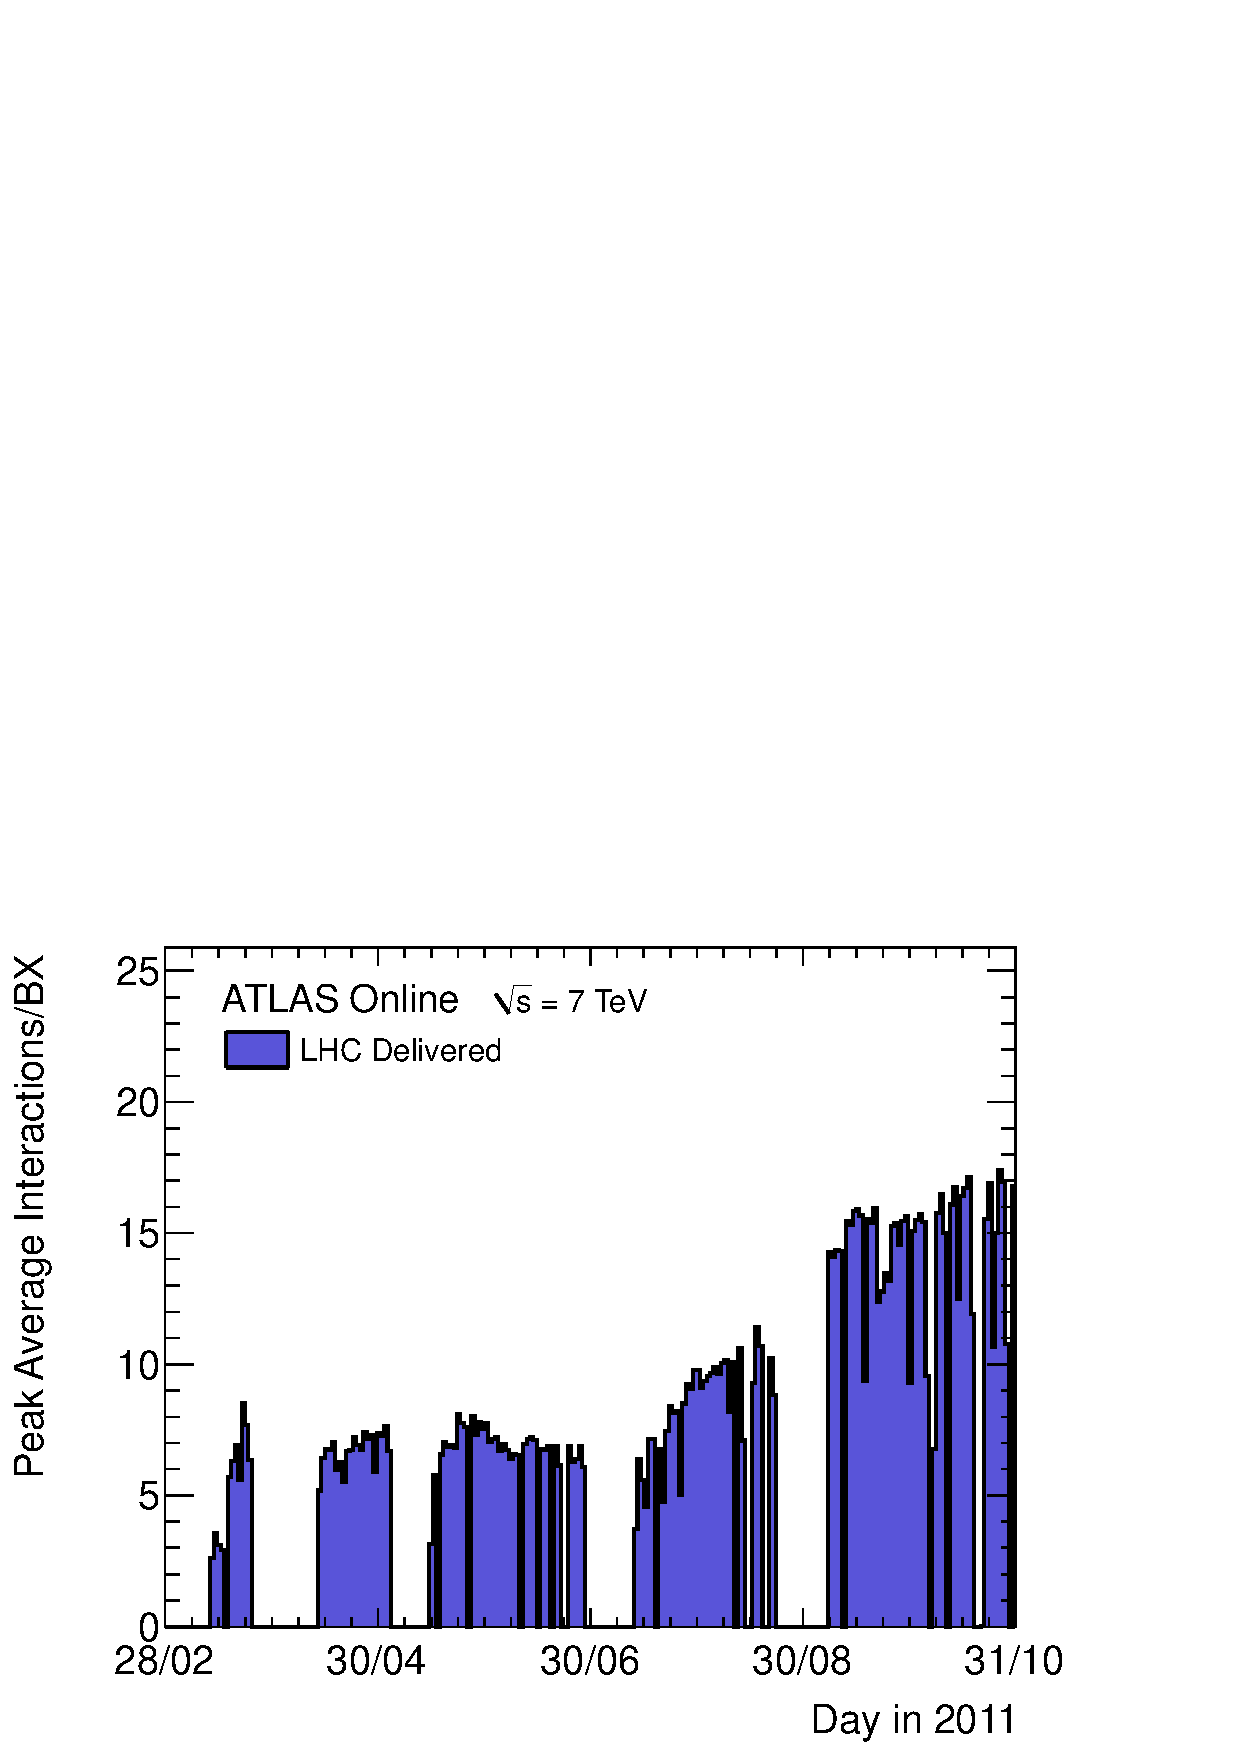
\includegraphics[width=0.7\textwidth]{Fig2/peakAvgMuByDay.pdf}
    \caption{Maximum mean number of events per beam crossing versus day in 2011}
    \label{fig:peakAvgMu}
  \end{center}
\end{figure}




%------------------------------------------------------------------------
\subsection{Luminosity and pile-up}\label{sec:lumiintro}
%------------------------------------------------------------------------

The rate of events produced by the colliding beams depends on the luminosity of the collisions, which is a measure of the number of events per second per unit cross section, typically measured in units cm$^2$s$^{-1}$. The number of events of a particular process, then, is given by the product of the integrated luminosity, $\int dt L$, and the cross section of the process, $\sigma_{event}$.  The integrated luminosities are typically quoted in units of inverse picobarns, pb$^{-1}$~=~10$^{-36}$cm$^{2}$. In order to measure processes with very little cross sections a very high luminosity is required. 

The delivered luminosity can be written as~\cite{ATLAS-CONF-2011-116}:

\begin{equation} 
\mbox{ {\it L }} = \frac{n_b f_r n_1 n_2 }{2\pi \Sigma_x \Sigma_y}
\label{eqn:lumi}
\end{equation} 
where n$_b$ is the number of colliding bunch pairs,  n$_1$ and n$_2$ are the bunch populations (protons per bunch) in beam 1 and beam 2 respectively (together forming the bunch charged product), $f_r$ is the machine revolution frequency, and $\Sigma_x$ and $\Sigma_y$ are the width and the height of the proton beams. %characterize the horizontal and vertical profiles of the colliding beams. 

The number of protons per bunch, the number of bunches per beam, and the revolution frequency are all set by the beam operators. The widths of the proton beams are measured in a process known as a Van der Meer ($vdM$) scan~\cite{vanderMeer:296752}. In a $vdM$ scan, the beams are separated by steps of a known distance. The collision rate is measured as a function of this separation, and the width of a gaussian fit to the distributions yields the width of the beams in the direction of the separation.  

The total integrated luminosities provided by the LHC and recorded by ATLAS in 2011 are shown in Figure~\ref{fig:integratedlumi}. These events form the dataset analyzed in this thesis. By means of the beam-separation or $vdM$ scans, as well as other techniques to measure the bunch charged product, the ATLAS Collaboration has determined that the uncertainty on its luminosity measurement is $\delta L = \pm 3.7$\%. For a complete description of the methods used and the systematic erros evaluated see reference~\cite{ATLAS-CONF-2011-116}.

\begin{figure}[htbp]
  \begin{center}
      \includegraphics[width=0.7\textwidth]{Fig2/sumLumiByDay.pdf}
    \caption{Total luminosity delivered by the LHC and recorded by ATLAS during the 2011 $sqrt{s}$ = 7~TeV proton-proton run}
    \label{fig:integratedlumi}
  \end{center}
\end{figure}


As anticipated, due to the cross-section for interaction and the number of protons per bunch, the possibility to observe multiple $pp$ interactions per bunch crossing increases proportionally. This phenomenon, referred to as ``pile-up'', can really occur in two distinct forms. The first form is the presence of multiple $pp$ collisions (different from the interaction of interest) in the same bunch crossing, referred to as ``in-time'' pile-up. The second form of pile-up takes place due to electronic integration times within the detector. Certain detector components are actually sensitive to multiple bunch crossings due to the long electronic signals generated in the response to energy depositions or charge collection. One or more $pp$ collisions in a bunch-crossing different from that which produced the collision of interest can then affect the measurement. This form of pile-up is referred to as ``out-of-time'' pile-up and will become more and more important as the LHC bunch spacing gets closer to the nominal value, 25~ns.

The fraction of events with pile-up increased significatively since the data taking started. The experimental signature of this fact is obtain via the number of reconstructed primary vertices, or NPV. The effect of the event NPV is an important concern for the measurement of jet properties and will be discussed in the next chapters.


%
%%%%%%%%%%%%%%%%%%%%%%%%%%%%%%%%%%%%%%%%%%%%%%%%%%%%%%%%%%%%%%%%%%%%%%%%%%%%%%%
% ATLAS
%%%%%%%%%%%%%%%%%%%%%%%%%%%%%%%%%%%%%%%%%%%%%%%%%%%%%%%%%%%%%%%%%%%%%%%%%%%%%%%
%
\section{The ATLAS Detector}

%------------------------------------------------------------------------
\subsection{Detector overview}\label{sec:atlassummary}
%------------------------------------------------------------------------
El dectector ATLAS, ac\'ronimo para A Toroidal LHC Apparatus, fue dise\~nado para estudiar la f\'isica de colisiones \emph{p-p} en el LHC. Todo el detector est\'a contenido en un cilindro de aproximadamente 44 metros de largo por 22 metros de di\'ametro y pesa unas 7000 toneladas\cite{TDR}.  Presenta una estructura tipo cebolla, pudiendo separarse en tres sistemas comenzando desde el punto de interacci\'on: el detector interno, los calor\'imetros y el sistema de muones (figura \ref{fig:ATLAS}) . Cada parte se divide a su vez en m\'as capas. Las part\'iculas emergentes atraviesan primero el detector interno, donde se reconstruye la trayectoria de las part\'iculas cargadas. En el calor\'imetro todas las part\'iculas, con excepci\'on de muones y neutrinos, depositan toda su energ\'ia y se detienen. Los muones interact\'uan electromagn\'eticamente al igual que los electrones, pero al ser mucho m\'as masivos que \'estos no emiten radiaci\'on de frenado y logran atravesar el calor\'imetro dando se\~nal en el sistema de detecci\'on de muones. ATLAS cuenta adem\'as con un sistema de imanes que provee de un campo magn\'etico que curva las trayectorias de las part\'iculas cargadas que atraviesan el detector interno y el espectr\'ometro de muones, permitiendo medir su momento.

   Todos los detectores de ATLAS, as\'i como el sistema de imanes, se componen de un barril central y dos tapas laterales id\'enticas. La cobertura en pseudorapidez de cada una de estas partes depender\'a del sistema considerado.

\begin{figure}[htbp]
  \begin{center}
      \includegraphics[angle=90,width=1\textwidth]{Fig2/TDRchapter1_fig1_ATLAS_DETECTOR.pdf}
    \caption{El detector de ATLAS}
    \label{fig:ATLAS}
  \end{center}
\end{figure}


%------------------------------------------------------------------------
\subsection{The Inner Detector}\label{sec:atlasID}
%------------------------------------------------------------------------
El detector interno de ATLAS (figura \ref{fig:figinner}) est\'a contenido en un cilindro de 7 m de longitud y 1,15 m de radio exterior. El mismo ha sido dise\~nado para la reconstrucci\'on de trazas de part\'iculas cargadas en un campo magn\'etico solenoidal de 2 Tesla, con un rango de pseudorapidez que se extiende hasta $|\eta|=  2.5$. Est\'a compuesto por tres subdetectores: el  detector de p\'ixeles , el detector de microbandas de silicio (SCT, del ingl\'es \emph{Semiconductor Tracker}) y el de transici\'on de radiaci\'on (TRT, \emph{Transition Radiation Tracker}).  La combinaci\'on de estas tecnolog\'ias permite el reconocimiento de trazas de manera robusta y una alta precisi\'on en las coordenadas $\eta$ y $\phi$.  

   Desde el punto de vista mec\'anico el detector consiste en un barril extendido en la coordenada \emph{z} sobre $\pm$ 80 cm, y dos ruedas o tapas laterales id\'enticas cubriendo el resto de la cavidad. En la regi\'on del barril todos los elementos de detecci\'on est\'an ordenados en estructuras cil\'indricas, mientras que en las tapas dichos elementos est\'an montados en discos perpendiculares a la direcci\'on del haz. Esto asegura que las part\'iculas pasen todos los elementos de detecci\'on con \'angulos de incidencia grandes.

\begin{figure}[htbp]
  \begin{center}
      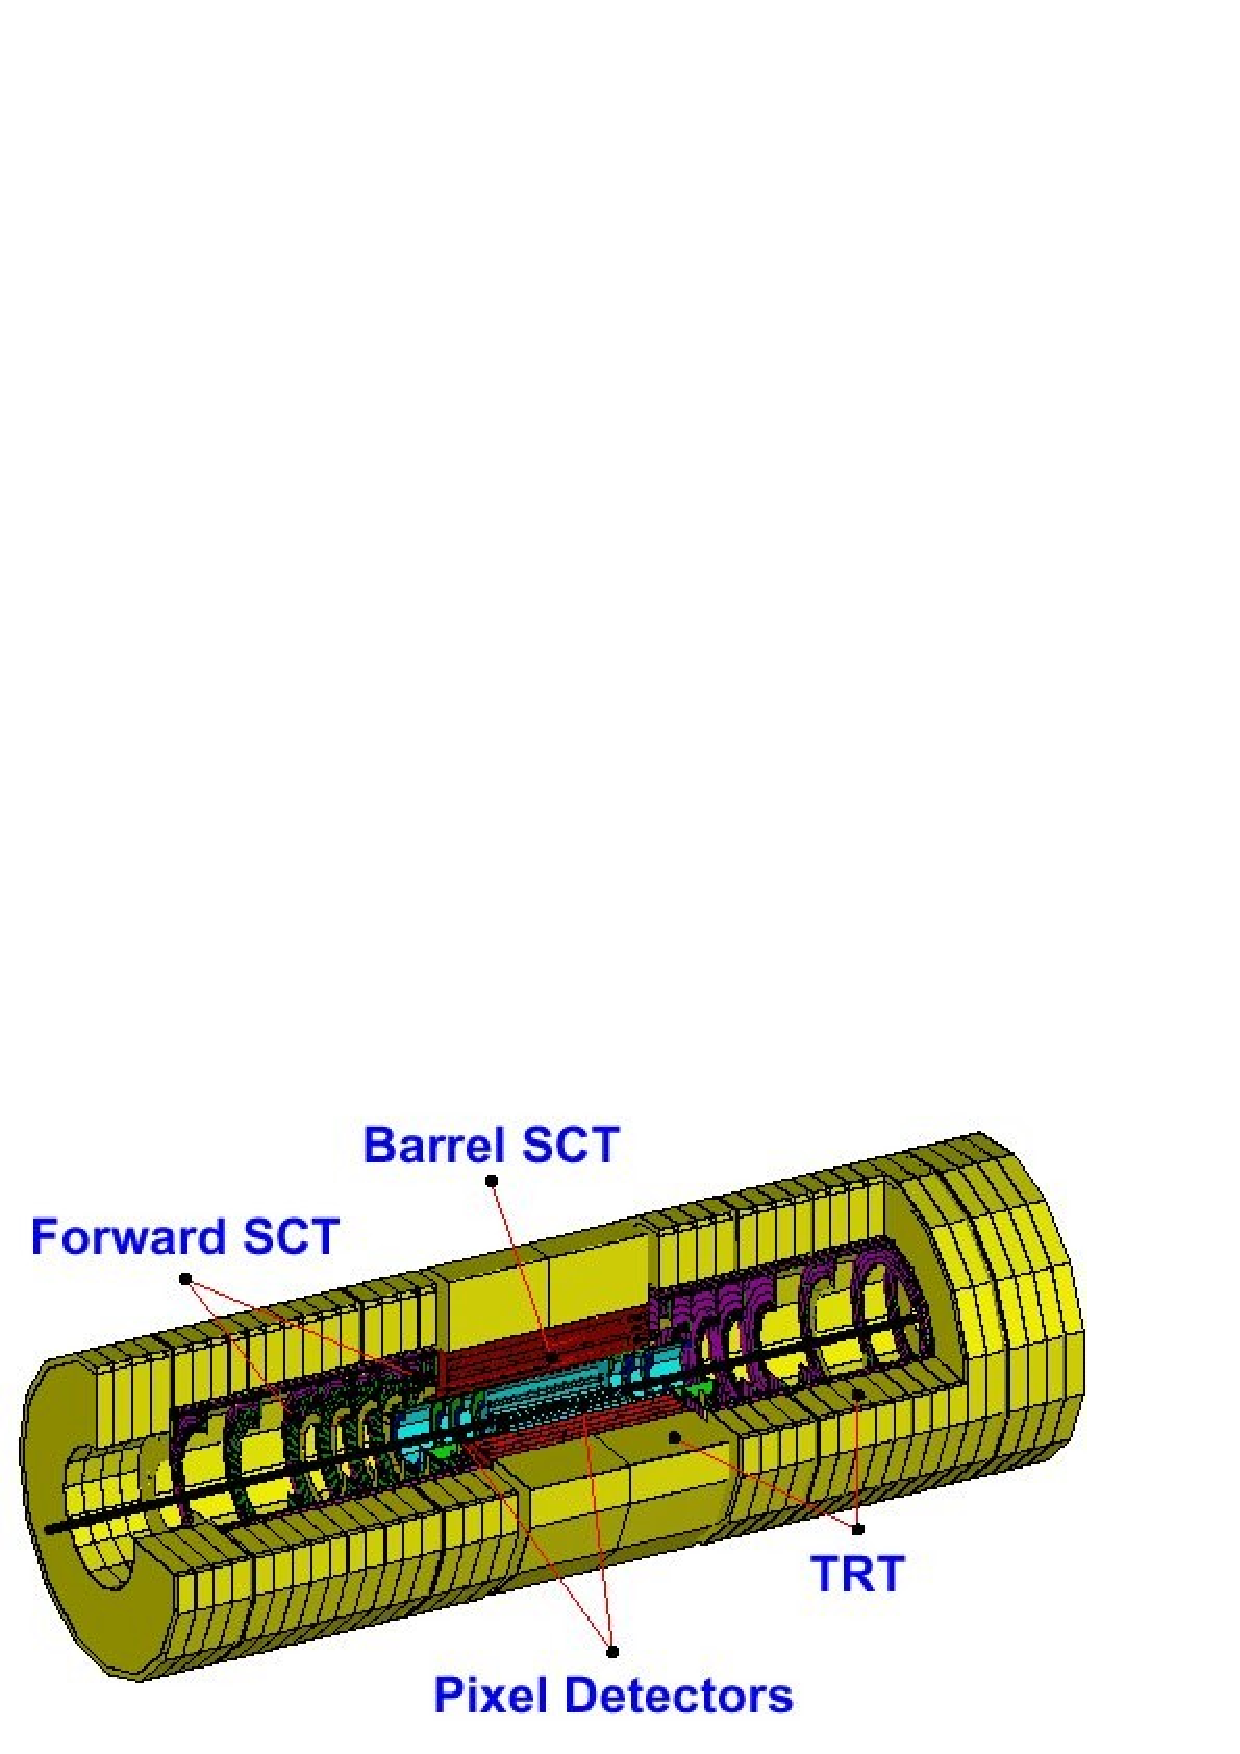
\includegraphics[width=0.9\textwidth]{Fig2/innnerdetector3d.pdf}
    \caption{Vista del detector interno de ATLAS. Se indican las posiciones del barril central y partes laterales del SCT, el detecor de p\'ixeles y el TRT}
    \label{fig:figinner}
  \end{center}
\end{figure}

%\subsubsection{Los detectores de  silicio}
%   El sistema de detectores de silicio est\'a dise\~nado  para proveer 11 mediciones de precisi\'on por traza en la regi\'on radial intermedia, contribuyendo a la medici\'on del momento, el par\'ametro de impacto y la posici\'on del v\'ertice.  Para ello dos tecnolog\'ias son implementadas: detectores de p\'ixel y detectores de microbandas de silicio. 

\subsubsection{El detector de p\'ixeles}

   Este sistema consiste en tres barriles de $\sim$ 4, 10 y 13 cent\'imetros de radio medio, respectivamente; y 5 discos a cada lado. Contiene 140 millones de elementos detectores de forma cuadradra,  cada uno de 50 $\mu$m en la direcci\'on R$\phi$ y 300 $\mu$m en z, midiendo as\'i dos coordenadas por cada m\'odulo detector. Todo el dispositivo est\'a situado tan cerca como es posible del punto de interacci\'on, entregando 3 mediciones de alta precisi\'on y granularidad en la regi\'on cercana al punto de interacci\'on primario, contribuyendo a la medici\'on del par\'ametro de impacto y la posici\'on del v\'ertice.

\subsubsection{El detector de microbandas de silicio}
% Ver esto

   El sistema de detecci\'on por microbandas de silicio consta de cuatro cilindros conc\'entricos; de 300, 373, 447 y 520 mm de radio, respectivamente, compuestos, cada uno de ellos, por  m\'odulos detectores montados en estructuras de fibra de carb\'on. Cada m\'odulo posee dos capas de microbandas. En la primera, las bandas est\'an dispuestas paralelas al eje del haz midiendo as\'i la cordenada $\phi$ directamente. \'Estas, junto con las microbandas en la capa siguiente, con un \'angulo \emph{stereo} de 40 mrad, reconstruyen la coordenada \emph{z}. A los lados del barril central se tienen dos tapas con m\'odulos montados en 9 ruedas. La resoluci\'on espacial en el sistema es de 16 $\mu$m en R$\phi$ y 580 $\mu$m en \emph{z}.

   %El sistema de detecci\'on por bandas de silicio consiste en 8 capas de dichas microbandas, dispuestas en m\'odulos, teniendo dos capas por cada m\'odulo detector. Estos  m\'odulos est\'an montados en estructuras cil\'indricas de fibra de carb\'on dando lugar a cuatro barriles de 300, 373, 447 y 520 mm de radio, respectivamente. En una de las capas del detector las bandas est\'an dispuestas paralelas al eje del haz midiendo as\'i la cordenada $\phi$ directamente. Esta capa, junto con las bandas en la capa posterior, con un \'angulo \emph{stereo} de 40 mrad, reconstruyen la coordenada \emph{z}. En las tapas, los m\'odulos detectores est\'an montados en anillos sobre nueve ruedas, que se encuentran tambi\'en unidas mediante un marco que las contiene.  La resoluci\'on espacial en el sistema de bandas es de 16 $\mu$m en R$\phi$ y 580 $\mu$m en \emph{z}. 

  Tendremos, t'ipicamente, 8 capas de bandas de silicio (m\'as las tres de p\'ixeles) atravesadas por cada traza proveniente del punto de interacci\'on. Un impacto (o \emph{hit}) en una de las capas se referir\'a a un canal de detecci\'on con una se\~nal de salida sobre un determinado umbral de energ\'ia. En el caso del detector de silicio, tendremos un cluster peque\~no de canales, creado por una part\'icula cargada o ruido. Dos impactos correspondientes a una misma traza, en las dos capas de un m\'odulo detector contribuyen a un punto tridimensional en el espacio que llamaremos SP, del ingl\'es \emph{Space Point}. 


\subsubsection{El detector de radiaci\'on de transici\'on}

   %ESTO ES MENOR
   %El detector de radiaci\'on de transici\'on se basa en el hecho de que cuando una part\'icula cargada atraviesa materiales con distinta constante diel\'ectrica emite radiaci\'on que depende del cociente energ\'ia a masa, permitiendo as\'i la identificaci\'on de las part\'iculas.
% el uso de hilos met\'alicos aislados contenidos en vol\'umens individuales de gas
 
  El detector de radiaci\'on de transici\'on de ATLAS est\'a basado en el uso de tubos detectores del di\'ametro de una pajita de gaseosa, para la identificaci\'on y reconstrucci\'on de las trayectorias de part\'iculas cargadas. En total hay alrededor de 370000 tubos de 4 mm de di\'ametro y 144 de longitud en todo el detector, y, en virtud de su peque\~no di\'ametro pueden operar a las altas frecuencias esperadas en el LHC. % llenados con una mezcla  gaseosa (70 $\%$ xen\'on), para la absorci\'on de la radiaci\'on de transici\'on.
   
  Cada tubo contiene en su interior un hilo de tungsteno, cubierto de oro, de 30 $\mu$m de di\'ametro y est\'a relleno de una mezcla gaseosa (70 $\%$ xen\'on) que se ioniza cuando pasa una part\'icula. La medici\'on del tiempo de arribo de los iones producidos al hilo central, permite determinar la posici\'on del impacto dentro del radio del tubo. %atravesado por dicha part\'icula. 
  Los tubos detectores est\'an orientados de manera radial (en ruedas) en las tapas y, a lo largo del eje del haz , en la regi\'on del barril. Estas orientaciones han sido elegidas para maximizar el n\'umero de tubos atravesados en todas las direcciones.  La secci\'on del barril consiste en m\'odulos individuales de entre 329 y 793 tubos axiales, cubriendo el rango radial de 56 a 107 cm.  

   La detecci\'on de radiaci\'on de transici\'on, provocada por la existencia de materiales de distinto \'indice de refracci\'on entre los tubos, generar\'a se\~nales m\'as intensas y permitir\'a una mejor identificaci\'on de electrones que atraviesan el detector (los muones tambi\'en emiten radiaci\'on de transici\'on pero al ser mucho m\'as masivos que los electrones, lo hacen en una cantidad mucho menor).

   Este sistema de detecci\'on por tubos provee un gran n\'umero de puntos por traza (t\'ipicamente 36 puntos), lo cual determina un seguimiento cont\'inuo de la misma, con mucho menos material por punto y menor costo (mucho menor comparado con la tecnolog\'ia de p\'ixeles implementada en el subdetector m\'as interno).  La gran cantidad de puntos o impactos por traza es un instrumento poderoso en la b\'usqueda y reconstrucci\'on de trazas en el detector interno.

%------------------------------------------------------------------------
\subsection{The Calorimeters}\label{sec:atlasCALO}
%------------------------------------------------------------------------
 El sistema de imanes superconductores de ATLAS consiste en un solenoide central que provee el campo magn\'etico necesario al detector interno, rodeado por un arreglo de bobinas o bucles, con forma de pista de carrera, que generan un campo magn\'etico toroidal para el espectr\'ometro de muones.Todo el sistema es enfriado de manera indirecta mediante el flujo de helio l\'iquido a 4,5 K.

   El solenoide es un electroim\'an superconductor de 5,3 m de largo, situado en el interior del calor\'imetro electromagn\'etico. Comparte el cri\'ostato con el calor\'imetro de arg\'on l\'iquido, evitando la presencia de dos paredes criost\'aticas y reduciendo as\'i la cantidad de material introducido. La longitud del solenoide es considerablemente m\'as peque\~na que la del barril del detector de trazas. Este es el resultado de un compromiso: un bobinado corto reduce la cantidad de material introducido mientras que uno largo proporciona un campo magn\'etico m\'as uniforme en dicho detector. El campo magn\'etico a lo largo del eje \emph{z} es de 2 T en el punto de interacci\'on.
% existe .criost\'aticas.?

   El arreglo de bobinas est\'a dividido en un barril central y dos regiones laterales, al igual que los detectores. El barril central est\'a constituido por 8 bobinas de 5 m de ancho por 25 metros de largo aproximadamente, dispuestas sim\'etricamente alrededor del haz de manera radial. Las bobinas del barril se encuentran en cri\'ostatos separdos, mientras que las 8 bobinas en cada una de las tapas o toroides laterales est\'an ubicadas en un cri\'ostato com\'un.

   Con un campo magn\'etico toroidal las part\'iculas atravesar\'an todo el rango de pseudorapidez casi perpendicularmente al haz. El n\'umero peque\~no de bobinas que generan el campo toroidal resulta en una intensidad de campo que var\'ia fuertemente con la coordenada $\phi$. En el barril el campo magn\'etico es de 2 T, mientras que en las tapas es de 4 T en las zonas de mayor intensidad.   
    
\subsubsection{El calor\'imetro}

   Una vez que la part\'icula atraviesa el detector interno, ingresa al calor\'imetro. Un detector calorim\'etrico est\'a dise\~nado para absorber la energ\'ia de las part\'iculas que lo atraviesan y se encuentra dividido normalmente en un calor\'imetro electromagn\'etico y uno hadr\'onico dado el diferente comportamiento de fotones/electrones por un lado, y hadrones por el otro.  As\'i el calor\'imetro de ATLAS consiste en un sector electromagn\'etico que cubre una regi\'on de pseudorapidez $|\eta|<3.2$ (barril y tapas),  y uno hadr\'onico formado por tres partes: un gran barril cubriendo la zona de $|\eta|<1.7$, dos tapas en los extremos cubriendo la regi\'on de $1.5<|\eta|<3.2$, y calor\'imetros de bajo \'angulo cubriendo la regi\'on de pseudorapidez de  $3.1 <|\eta|< 4.9$. % Para la identificaci\'on de energ\'ia transversa faltante el calor\'imetro debe constar de una alta hemeticidad lo que significa que la cobertura en pseudorapidez debe alcanzar $|\eta|<5$. 

\subsubsection{El calor\'imetro de arg\'on l\'iquido}
  
   El calor\'imetro electromagn\'etico de ATLAS consiste en un gran barril interno y dos ruedas (\emph{end-caps}), una a cada lado del mismo. Se trata de un calor\'imetro de muestreo que funciona con arg\'on l\'iquido (se denomina de muestreo porque mide s\'olo una fracci\'on de la energ\'ia depositada por la part\'icula incidente). Est\'a formado por placas de plomo/acero inoxidable intercaladas con electrodos de cobre; el espacio entre ambos se llena con arg\'on l\'iquido, permitiendo la deriva de los electrones de ionizaci\'on bajo el alto voltaje aplicado. 

  Con el fin de asegurar una perfecta cobertura en todo el rango de pseudorapidez  y proveer una completa simetr\'ia en la coordenada $\phi$ se ha elegido una geometr\'ia en forma de acorde\'on. En la regi\'on dedicada a f\'isica de precisi\'on ($|\eta|<2.5$) el calor\'imetro electromagn\'etico est\'a dividido en cuatro secciones de muestreo. La primera o \emph{Presampler} consiste en una delgada capa de arg\'on desprovista de material absorbente, cuyo prop\'osito es la correcci\'on por la p\'erdida de energ\'ia  en el solenoide y las paredes del cri\'ostato. La segunda secci\'on posee una profundidad de 4.3$X_{0}$\footnote{$X_{0}$ es el s\'imbolo utilizado para la Longitud de Radiaci\'on (\emph{Radiation length}), definida como la distancia media sobre la cual un elect\'on muy energ\'etico pierde $1/e$ de su energ\'ia por bremsstrahlung o bien, como $7/9$ del camino libre medio en la producci\'on de pares. Contituye una escala de longitud apropiada para describir cascadas electromagn\'eticas de alta energ\'ia.} y en ella la lectura se lleva a cabo mediante celdas en forma de tiras delgadas en $\eta$, dando una buena resoluci\'on en dicha coordenada, con $\Delta\eta=0.0031$. La secci\'on de \emph{2nd Sampling} (16$X_{0}$) es donde se deposita la mayor\'ia de la energ\'ia, teniendo ambas coordenadas igual importancia. All\'i el tama\~no de celda es de $\Delta\phi\Delta\eta=0.0245\times 0.0245$. S\'olo los electrones m\'as energ\'eticos llegar\'an a la cuarta secci\'on de muestreo (\emph{3rd Sampling}).

   Las ruedas calorim\'etricas comienzan en $|\eta|=1.5$ y contin\'uan abajo hasta $|\eta|=3.2$, pero con un tama\~no de celda mayor por encima de $|\eta|=2.5$.

   En la regi\'on de bajo \'angulo, el calor\'imetro hadr\'onico funciona tambi\'en con arg\'on l\'iquido de manera de resistir los altos niveles de radiaci\'on. Su dise\~no es m\'as sencillo que el del calor\'imetro electromagn\'etico y como absorbentes posee placas paralelas de cobre, perpendiculares al haz. La regi\'on de esta parte del calor\'imetro hadr\'onico, que cubre hasta $|\eta|=4.9$, est\'a hecha de cobre/tungsteno. La elecci\'on de este material es necesaria para limitar el ancho y la profundidad de las lluvias provenientes de jets de altas energ\'ias cercanas a la l\'inea del haz. %and to sep the background levels low in the surrounding calorimeteres from particles spraying out from the forward region.

\subsubsection{El calor\'imetro hadr\'onico de tejas}
% TileCal [ ] Tile Calorimeter Technical Design Report, CERN/LHCC 96-42, 15-12-1996;

   El calor\'imetro hadr\'onico de tejas de ATLAS est\'a compuesto por tres barriles, uno central de 5,6m y dos extensiones de 2,9m cada una. El radio interno es de 2,2m y el externo, de 4,2m.  

   Cada barril est\'a dividido en 64 cu\~nas azimutales o m\'odulos, con una estructura peri\'odica en la direcci\'on paralela al haz. Cada m\'odulo es una estructura de tejas de hierro (material absorbente) alternadas con tejas de pl\'astico centellador, dispuestas en un plano paralelo al eje del haz.  Los materiales centelladores emiten luz en forma de peque\~nos pulsos cuando son atravesados por part\'iculas o radiaci\'on; acoplando el centellador a un fotomultiplicador el pulso de luz se convierte en un pulso el\'ectrico que puede ser analizado.  En el caso del calor\'imetro hadr\'onico de ATLAS, cuando una part\'icula atraviesa una teja centelladora emite luz en el rango del ultravioleta, de intensidad proporcional a la energ\'ia depositada por la part\'icula. 

   Se ha elegido una segmentaci\'on proyectiva en torres de $\Delta\phi\Delta\eta=0.1\times 0.1$ y cada una de estas torres est\'a dividida, en profundidad, en tres celdas, le\'idas individualmente por dos fotomultiplicadores para conseguir redundancia en la se\~nal. La luz generada en las tejas es recogida mediante fibras \'opticas que cambian la longitud de onda y transportada a los fotomultiplicadores (este subdetector posee unos 10.000 fotomultiplicadores).

   El calor\'imetro hadr\'onico debe tener el espesor suficiente para contener la energ\'ia de los hadrones. Con este prop\'osito y para obtener una buena resoluci\'on se han elegido 11 longitudes de absorci\'on como camino previo a las c\'amaras de muones.
 

%------------------------------------------------------------------------
\subsection{The Muon System}\label{sec:atlasCALO}
%------------------------------------------------------------------------
 El sistema de muones sirve a un doble prop\'osito: funciona como sistema de disparo (o \emph{trigger}) para la selecci\'on de eventos con muones de alta energ\'ia, y como espectr\'ometro de muones de alta precisi\'on. En este sentido, este detector llevar\'a a cabo la identificaci\'on de los muones producidos en las colisiones \emph{p-p}, determinando sus trayectorias y momentos.
% Las part\'iculas provenientes del punto de interacci\'on atraviesan tres conjuntos de c\'amaras, uno situado previo al toroide, uno interior y otro posterior. 
   El sistema consiste en un conjunto de toroides (llamamos as\'i, por su forma, a los tres conjuntos de bobinas que proveen el campo magn\'etico toroidal) y c\'amaras de tubos de deriva que se encuentran rodeando al calor\'imetro. En la parte del barril del detector, las c\'amaras est\'an situadas en el interior del toroide lo que permite la medici\'on del momento de las part\'iculas a partir de la desviaci\'on de sus trayectorias en el campo magn\'etico. En las tapas, donde la presencia del cri\'ostato impide posicionar las c\'amaras dentro del campo magn\'etico, el momento es medido a partir de la diferencia entre los \'angulos de entrada y salida del im\'an.
En el plano trasversal, tanto en la regi\'on del barril como en las tapas laterales, el sistema de c\'amaras estar\'a dividido en 16 sectores, siguiendo la simetr\'ia determinada por las 8 bobinas del barril central del sistema magn\'etico. Las c\'amaras cubren el espacio entre las bobinas, y todo el rango acimutal en la regi\'on que las rodea. Los sectores se numeran comenzando a partir de $\phi = 0$, en el sentido contrario de las agujas del reloj, teniendo en la direcci\'on vertical a los sectores 6 (en la parte superior del detector) y 13 (sector inferior).  

   Los c\'amaras de tubos de deriva (MDTs) son c\'amaras proporcionales hechas de tubos de aluminio de 30 mm de di\'ametro y longitudes variables de 70 a 630 cm, con un hilo central de 50$\mu$m de di\'ametro, de W-Re. En la regi\'on del barril dichas c\'amaras est\'an distribuidas en 3 capas cil\'indricas conc\'entricas (estaciones) alrededor del haz, de 5; 7,5 y 10 metros de radio. Los tubos est\'an dispuestos de manera transversal al eje \emph{z} de manera de medir la coordenada en el plano de desviaci\'on de la trayectoria de la part\'icula (plano \emph{Rz}).  Estas c\'amaras miden el tiempo de deriva de la ionizaci\'on producida por el paso del mu\'on, teniendo una resoluci\'on de 80 $\mu$m.
% MAS del TDR? Falta los radios de las estaciones(?)
   
   Cada c\'amara MDT est\'a cubierta por una o dos c\'amaras de placas resistivas (RPCs). Cada una de ellas encierra un volumen de gas entre planchas resistivas de baquelita, dotada una de ellas con tiras de electrodos. Dado que los tubos de deriva poseen un di\'ametro relativamente grande que resulta en un tiempo de deriva m\'aximo de 480ns, mucho mayor que los 25 ns entre cruce de \emph{bunches}, se requieren c\'amaras especiales de disparo para la selecci\'on de eventos. La funci\'on de trigger en el barril es provista por tres capas de RPCs, situadas, dos de ellas, a ambos lados de la segunda estaci\'on de MDTs y la restante, en la cara interior de la estaci\'on m\'as externa. 
En las tapas, esta funci\'on es cumplida por tres estaciones de TGCs (\emph{Thing Gap Chambers}). Estas c\'amaras son similares en dise\~no a c\'amaras prporcionales multihilo, con la diferencia de que poseen una distancia c\'atodo-c\'atodo menor que la pendiente del \'anodo (hilo). 
   Las c\'amaras de disparo proveen una estimaci\'on de las coordenadas $\phi$ y $\eta$ del punto de impacto de la traza, mientras que las c\'amaras MDTs dar\'an (con mayor precisi\'on) la coordenada $\eta$.

    En la regi\'on de bajo \'angulo, donde la densidad de trazas es mayor, se utilizan c\'amaras de tiras de c\'atodos (CSCs) de granularidad m\'as fina comparadas con las MDTs, para la detecci\'on de trayectorias. Estas c\'amaras son c\'amaras proporcionales, con un espacio entre hilo de 2,5 mm. Cada una de ellas proporciona medida de dos coordenadas y puede operar en condiciones de alto campo magn\'etico.

   En la figura \ref{fig:MUON1} se puede ver un esquema del espectr\'ometro de muones, donde se indica la posici \'on de las diferentes c\'amaras descriptas.

\begin{figure}[htbp]
  \begin{center}
      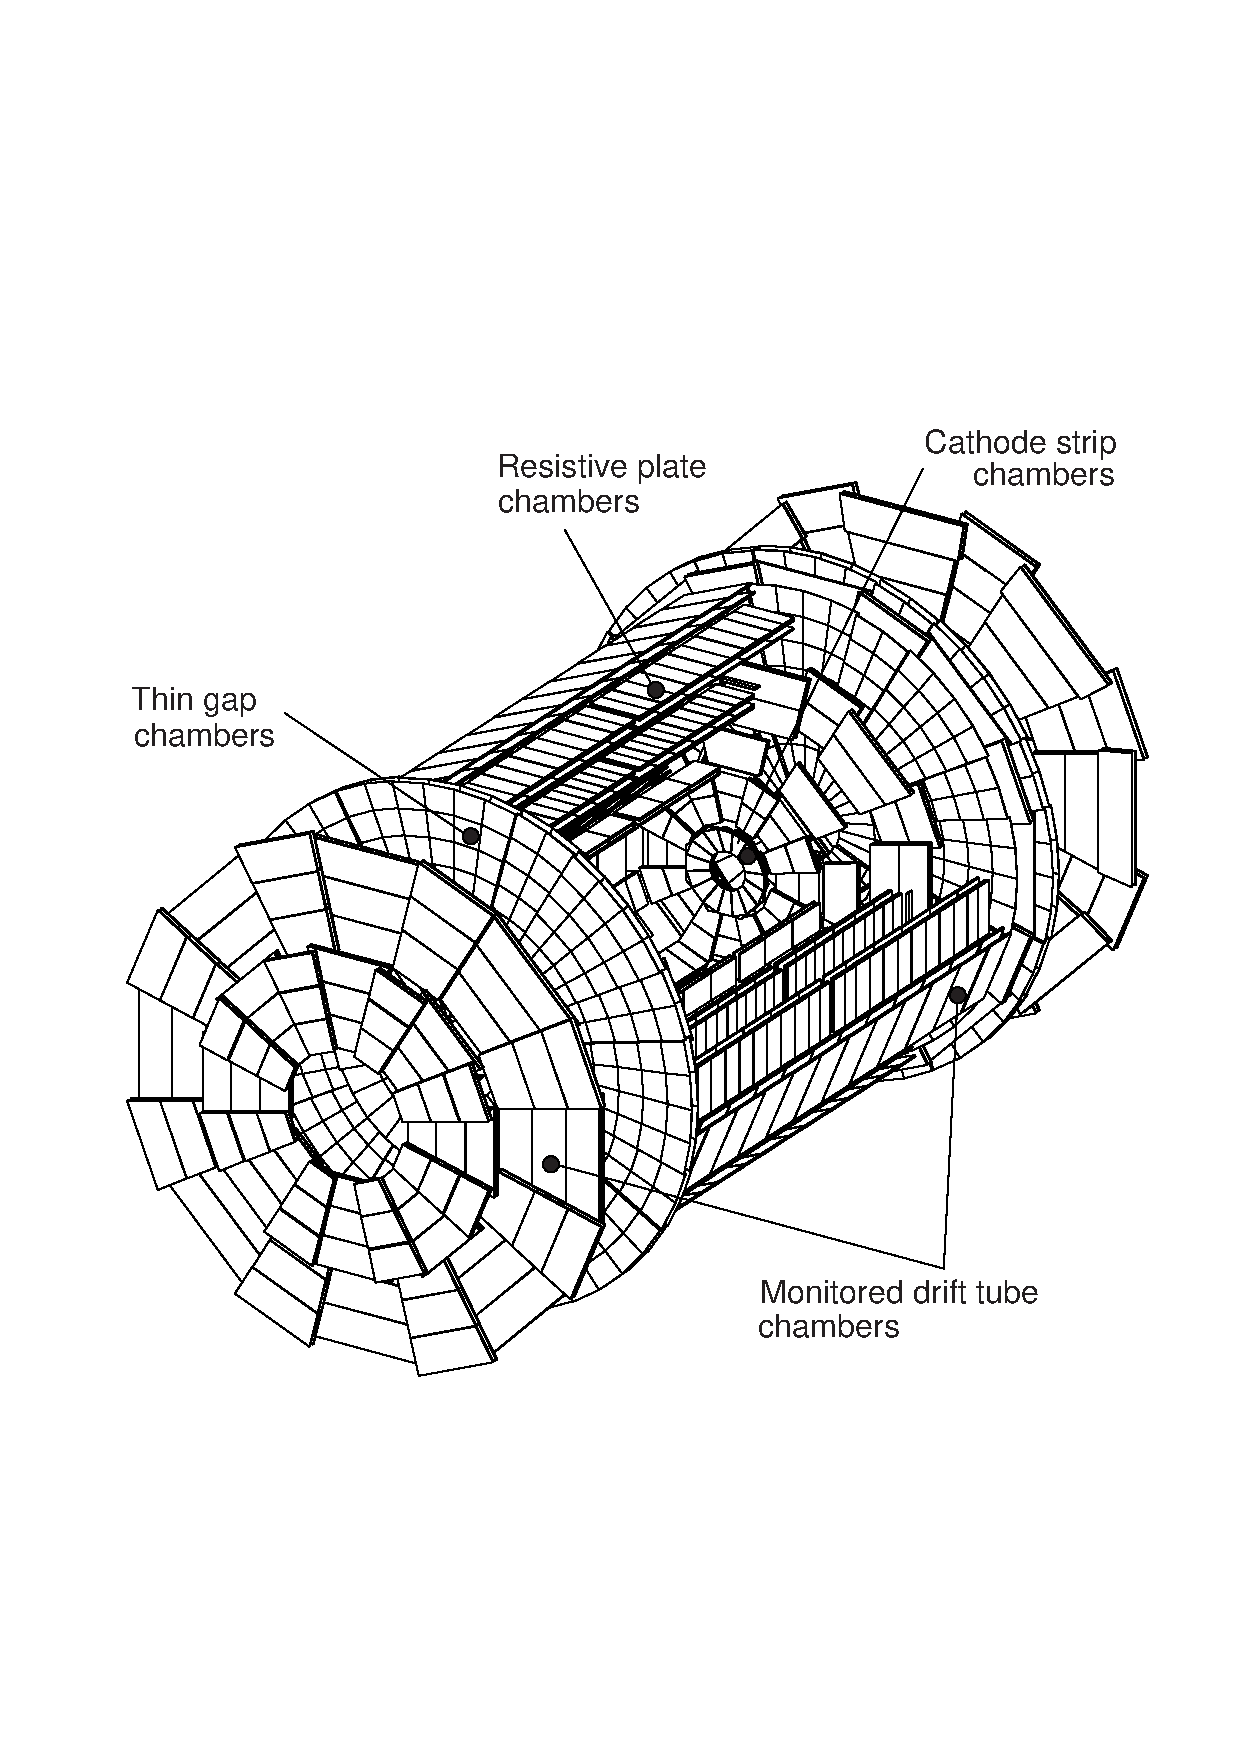
\includegraphics[width=0.8\textwidth]{Fig2/muonspectrometeradele-bw.pdf}
    \caption{Vista tridimensional del espectr\'ometro de muones de ATLAS, indicando las \'areas cubiertas por las diferentes c\'amaras que lo componen}
    \label{fig:MUON1}
  \end{center}
\end{figure}



%------------------------------------------------------------------------
\subsection{Trigger and Data Adquisition}\label{sec:atlasCALO}
%------------------------------------------------------------------------
 En este cap\'itulo se analiza la estructura del trigger de ATLAS, y el sistema de adquisici\'on y flujo de los datos. Se presenta, asimismo, una breve descripci\'on de los algoritmos usados en la reconstrucci\'on de trayectorias para la selecci\'on de eventos en el detector interno. 


\subsubsection{Arquitectura general}

   El sistema de Trigger y Adquisici\'on de Datos\cite{TDRtdaq} de ATLAS est\'a basado en tres niveles de selecci\'on \emph{online}: Nivel 1, Nivel 2 y Filtro de Eventos. Cada nivel es m\'as lento pero m\'as preciso que el anterior. Trabajando con una frecuencia de interacci\'on de $10^{9}$ Hz y luminosidades del orden de $10^{34}$ $cm^{-2}$ $s^{-1}$, este sistema ser\'a el encargado de reducir la frecuencia de eventos inicial de 40 MHz a 200Hz, que es la velocidad con la que pueden almacenarse. 

   En la figura \ref{fig:TDAQ} se muestra un vista simplificada de los principales componentes y funciones.  

\begin{figure}[!h]
\begin{center}
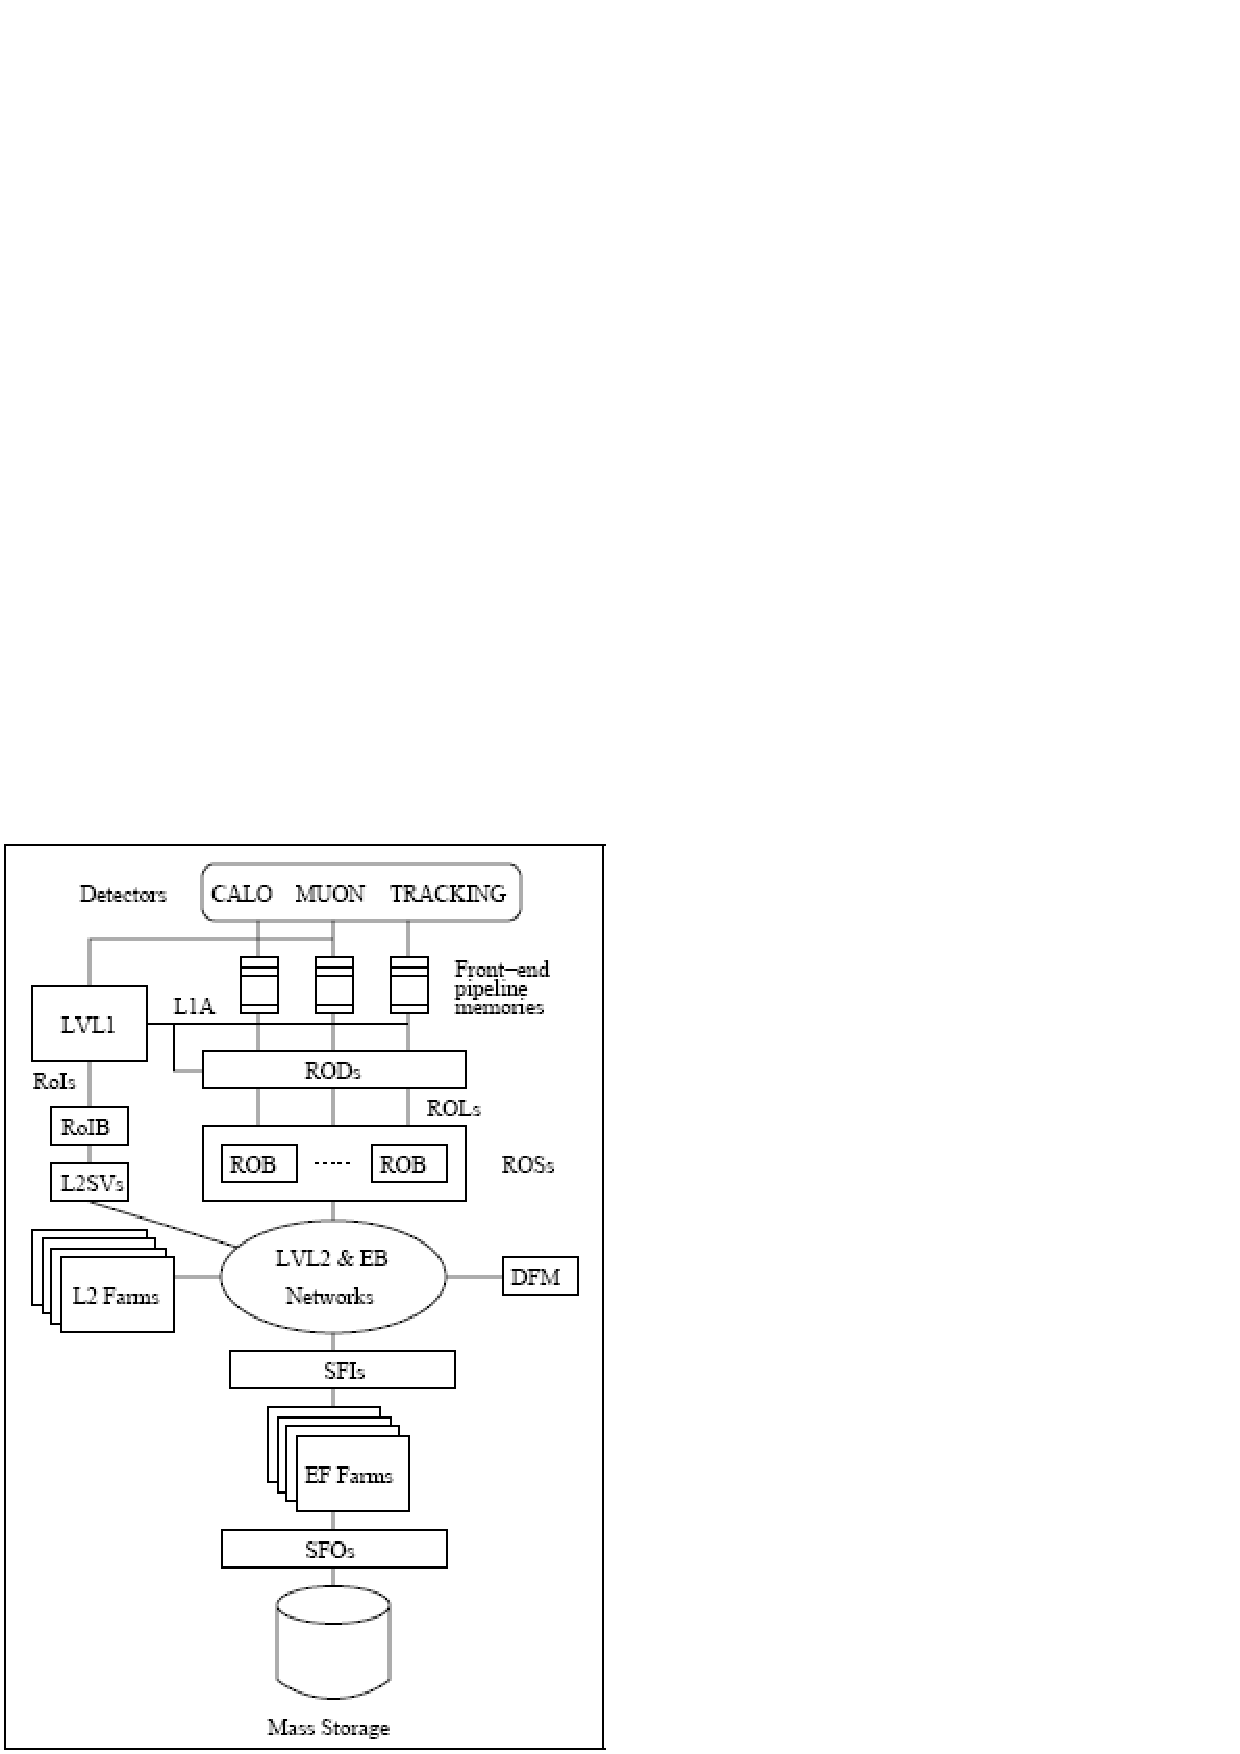
\includegraphics[width=0.5\textwidth]{Fig3/paint_TDAQ.pdf}
\caption{Principales componentes del sistema de trigger y adquisici\'on de datos de ATLAS. } 
\label{fig:TDAQ}
\end{center}
\end{figure}

   El mecanismo que lleva a cabo el movimiento de la informaci\'on (Data Flow System), es el responsable de recibir los datos de los detectores, pasando parte de ellos al sistema de trigger y enviando luego, los eventos seleccionados al lugar de almacenamiento. Siguiendo el esquema de la figura, la comunicaci\'on entre los \emph{drivers} de lectura %controladores de lectura?
de cada detector (RODs) y el sistema de adquisici\'on de datos, est\'a dada por los \emph{buffers} de almacenamiento transitorio (ROBs). La informaci\'on de los eventos aceptados por el Nivel 1 son transportados de los primeros al sistema de lectura (ROS), que consta de numerosos ROBs, guardando los datos a la espera de la decisi\'on del trigger. La informaci\'on requerida por el segundo nivel es provista por estos \'ultimos. Los eventos aceptados son reconstruidos (a partir de fragmentos contenidos en diferentes ROBs) y pasados al siguiente nivel.
%(\emph{Read Out Drivers})
%(\emph{Read Out Buffers})
% (\emph{Read Out System})

   El Nivel 2 y el Filtro de Eventos componen el \emph{High-level Trigger} (HLT) de ATLAS. El Nivel 2 trabaja a la frecuencia de aceptaci\'on del Nivel 1, utilizando una secuencia de r\'apidos algoritmos de selecci\'on que operan t\'ipicamente sobre una fracci\'on de los datos del evento, contenida en regiones del detector previamente seleccionadas por ese nivel (ver el mecanismo de la regi\'on de inter\'es en la siguiente secci\'on). Si la decisi\'on del Nivel 2 es rechazar el evento, los datos del mismo son eliminados de los buffers correspondientes. Si el evento es aceptado,  se reconstruye  en el EB (Event Builder) y es pasado al Filtro de Eventos. Este nivel ejecutar\'a algoritmos de reconstrucci\'on m\'as sofisticados, adaptados de aquellos para el an\'alisis \emph{offline}, utilizando informaci\'on detallada de los detectores para efectuar el proceso de selecci\'on final, que determinar\'a cu\'ales son los eventos que ser\'an guardados para posteriores estudios.

  En las siguientes secciones se presenta una descripci\'on m\'as detallada de los niveles de trigger.

 
\subsubsection{El Nivel 1}

   El primer nivel de trigger de ATLAS es implementado mediante hardware. \'Este realiza una decisi\'on inicial a partir de la informaci\'on provista por los calor\'imetros y del detector de muones, basando su estrategia en la combinaci\'on de objetos en coincidencia. %or veto.
  
   En el sistema de muones, los candidatos de alto momento transverso son identificados en las c\'amaras especiales de trigger: RPCs en el barril y TGCs en las tapas. En el caso del calor\'imetro, se definen una serie de conjuntos de umbrales de $p_T$ para cada objeto (electrones, fotones, jets, etc.), seleccionando aquellos que pasen los criterios de selecci\'on correspondientes al evento f\'isico de inter\'es. 

   Puesto que la decisi\'on de aceptar un evento no puede ser realizada en los 25 ns que median entre dos cruces de \emph{bunches}, los subdetectores almacenan localmente la informaci\'on del mismo en \emph{pipelined buffers} hasta que el Nivel 1 efect\'ua la selecci\'on. Luego, los datos son enviados a los RODs especi\'ficos de cada detector para luego dirigirse a los ROBs, donde son almacenados hasta que la decisi\'on del Nivel 2 sea alcanzada. 
   Cuando un evento es aceptado, el Nivel 1 comunica la decisi\'on al mecanismo que se encargar\'a de construir una Regi\'on de Inter\'es (RoI). Este mecanismo es una importante pieza sobre la que descansa la estrategia del sistema de trigger; a trav\'es del mismo, el Nivel 2 har\'a uso de la informaci\'on del evento en regiones localizadas del detector, de manera que los algoritmos de reconstrucci\'on en ese nivel s\'olo transfieran los ROBs necesarios para arribar a una r\'apida decisi\'on. %Es importante notar que la informaci\'on de todos los subdetectores est\'a disponible para dichos algoritmos en caso de ser necesario.
La RoI contendr\'a la informaci\'on de la posici\'on ($\eta$ y $\phi$) y el momento de los objetos candidatos.

   Este nivel est\'a dise\~nado para llevar a cabo su decisi\'on en un tiempo menor a 2.5 $\mu$s, medidos desde la colisi\'on \emph{p-p}, hasta que la informaci\'on del evento est\'a disponible en la electr\'onica de salida de los detectores. En este proceso la frecuencia de eventos ser\'a reducida a 75KHz (l\'imite fijado por la electr\'onica).

\subsection{El HLT}

 El High-level Trigger de ATLAS abarca la segunda y tercera etapa de la selecci\'on de eventos. Comprende el Nivel 2 y el Filtro de Eventos, y contiene adem\'as, el Software de Selecci\'on (ESS). Este \'ultimo comparte la estructura usada por el Offline para los c\'odigos de selecci\'on, facilitando el an\'alisis \emph{offline} de los datos, y el desarrollo de algoritmos en el HLT.

   El punto de entrada del trigger es el resultado del Nivel 1. \'Este provee informaci\'on acerca de la regi\'on de inter\'es, fundamental para el r\'apido funcionamiento de los algoritmos del Nivel 2. As\'i, los datos del Nivel 1 gu\'ian la selecci\'on del Nivel 2; y \'esta a su vez guiar\'a la del Filtro de eventos, como se ilustra en la figura \ref{fig:HLTchainseed}. 
%HLTchain_seeding.pdf
\begin{figure}[!h]
\begin{center}
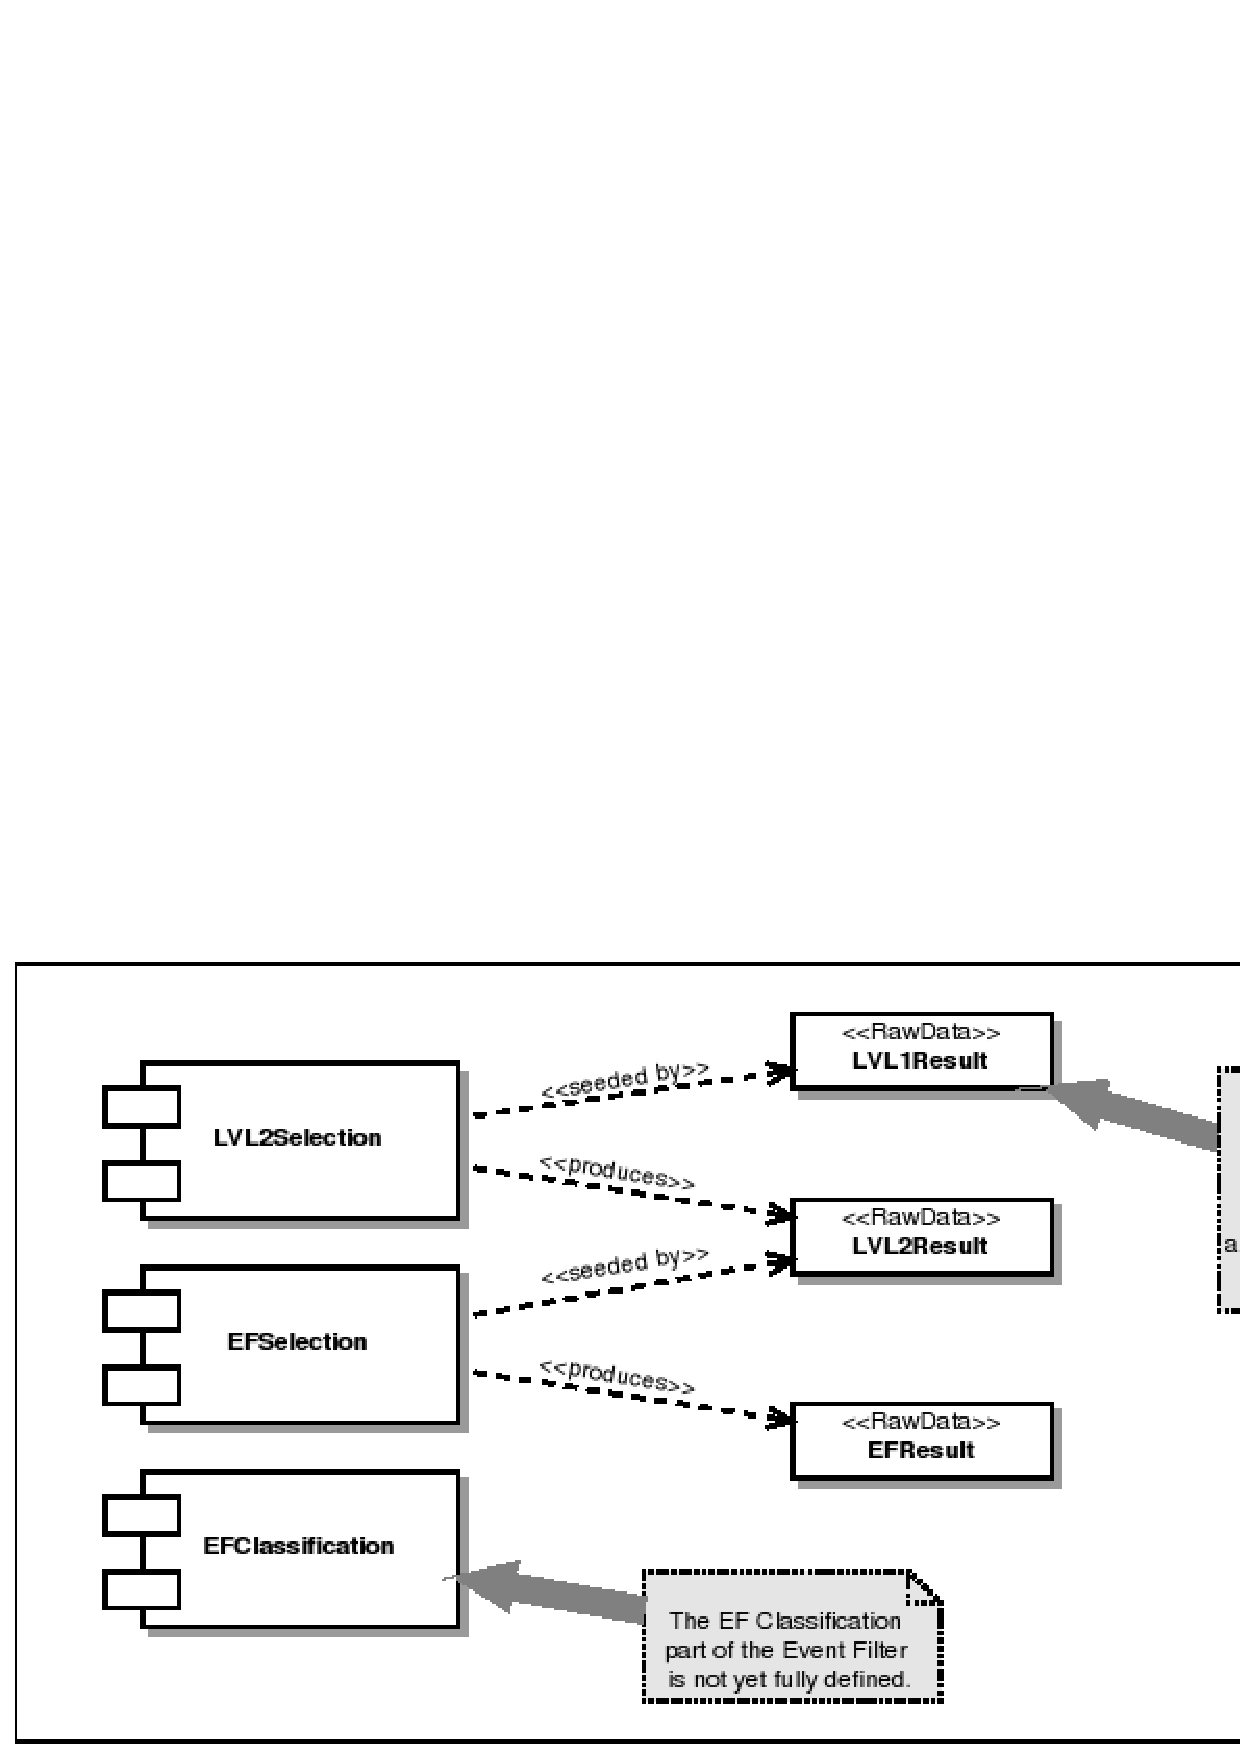
\includegraphics[width=0.9\textwidth]{Fig3/HLTchain_seeding.pdf} 
\caption{Cadena de selecci\'on del \emph{High-level Trigger} de ATLAS. Cada nivel es guiado por el resultado del paso anterior.}
\label{fig:HLTchainseed}
\end{center}
\end{figure}


\subsubsection{El Nivel 2}
   La tarea espec\'ifica del Nivel 2 es reducir la frecuencia de eventos de $\sim$ 100 kHz a alrededor de 2 kHz, combinando la informaci\'on de todos los detectores para su decisi\'on global. A diferencia del Nivel 1, esta segunda etapa de selecci\'on realiza operaciones no sincronizadas sobre los eventos, con un tiempo de decisi\'on de 10 ms.
%asynchronous??

   El Nivel 2 utiliza las regiones de inter\'es provistas por el Nivel 1. Cada regi\'on es examinada en el subdetector de origen (calor\'imetro o sistema de muones) para su confirmaci\'on; para luego buscar informaci\'on de otros subdetectores. En el caso del trigger de muones, el poder de rechazo del Nivel 2 proviene de ajustar los umbrales de $p_{T}$, respecto de los utilizados en el primer nivel, a partir de la informaci\'on de las c\'amaras de precisi\'on del sistema de muones (MDTs) y la correspondiente al detector interno.
Los procesadores del Nivel 2 son los encargados de ejecutar luego el software de selecci\'on de eventos, utilizando la informaci\'on almacenada en los \emph{buffers}. Usando las RoIs del Nivel 1, el Nivel 2 acceder\'a de manera selectiva a los datos en los ROBs, moviendo s\'olo la informaci\'on requerida para efectuar la decisi\'on. T\'ipicamente, s\'olo una peque\~na fracci\'on del detector, correspondiente a las regiones centradas en los objetos indicados por el Nivel 1, ser\'an necesitados por el segundo nivel.

  Hasta que un evento es aceptado o rechazado (en $\sim$ 10 ms), los datos son retenidos en los ROBs. En caso de aceptaci\'on, los fragmentos del evento almacenados en distintos buffers ser\'an requeridos por el sistema de control del Nivel 2 (L2SVs) para ser enviados al constructor de eventos (EB). El evento ensamblado es guardado en una \'unica direcci\'on de memoria para ser utilizado por el Filtro de Eventos. El tama\~no promedio de un evento ser\'a del orden de 1,5 MB.


\subsubsection{El Filtro de Eventos}

  Luego del Nivel 2, la \'ultima etapa de selecci\'on \emph{online} es realizada por el Filtro de Eventos (EF). El EF emplea algoritmos y m\'etodos similares a los implementados en el an\'alisis \emph{offline}, adaptados para su corrida en el tiempo real del experimento; su poder de rechazo radica en el uso de algoritmos y criterios de selecci\'on m\'as complejos, que por l\'imites en el tiempo de procesamiento no pueden ser utilizados en el Nivel 2.
  
  El EF utilizar\'a informaci\'on actualizada de la calibraci\'on y alineamiento del detector y un completo mapa del campo magn\'etico; llevando a cabo con ello la selecci\'on final del evento f\'isico que ser\'a guardado para su estudio en el Offline. La frecuencia de aceptaci\'on del nivel anterior ser\'a reducida en un orden de magnitud, almacenando a una tasa de $\sim$100 MB/s.


\subsubsection{El software de selecci\'on}
\label{'HLTalgos'}
   
 La tarea del software de selecci\'on (ESS) es la selecci\'on y clasificaci\'on de los eventos. Candidatos tales como electrones, jets, muones, etc., representados por objetos abstractos, son reconstruidos utilizando un particular conjunto de algoritmos. Un evento es seleccionado si el objeto reconstruido satisface al menos una de las signaturas establecidas en el men\'u del sistema de disparo. En el Nivel 2 y el Filtro de Eventos (EF), los eventos ser\'an rechazados si no pasan los espec\'ificos criterios de selecci\'on, dise\~nados para la reducci\'on de la frecuencia de eventos, al l\'imite dado por la velocidad a la que \'estos pueden ser almacenados.

 El ESS se compone de una infraestructura y un conjunto de programas de selecci\'on para las dos etapas del HLT.  Los algoritmos de reconstrucci\'on para el trigger est\'an basados en aquellos utilizados para la reconstrucci\'on \emph{offline}, pero correr\'an \emph{online} en el entorno de software provisto por los procesadores del Nivel 2 y el EF. 

  De manera de facilitar el desarrollo de los algoritmos del HLT y simplificar los estudios del Offline; el ESS ha sido dise\~nado de manera de poder ser ejecutado directamente en el entorno provisto por la estructura de software de an\'alisis offline del experimento, ATHENA\cite{Athena}. La estructura dada por este paquete de software es lo suficientemente flexible como para abarcar una variedad de procesos, incluyendo no s\'olo algoritmos de trigger sino tambi\'en tareas de calibraci\'on y monitoreo. Se ha destinado un ap\'endice (A) para su descripci\'on.
 
  En el Offline, la tarea del ESS es la de emular la cadena completa de selecci\'on \emph{online}. Para su ejecuci\'on el sistema se sirve de cuatro sub-paquetes: el direccionamiento o \emph{Steering}, los algoritmos del HLT, y los paquetes de software para la clasificaci\'on y movimiento de los datos, EDM (\emph{Event Data Model}) y el DM (\emph{Data Manager}). Los \'ultimos toman los datos del evento en el formato que poseen a la salida de los sistemas de lectura (\emph{Raw data} en formato \emph{byte stream}), y los convierten en objetos que puedan ser usados por los algoritmos en la cadena de selecci\'on (\emph{Raw Data Objects}).

  La tarea de los algoritmos del HLT es la de analizar los datos del evento, reconstruyendo partes del mismo, luego de la selecci\'on del Nivel 1. El paquete se compone de dos subconjuntos principales:
%itemize
\begin{itemize}
   \item Programas de preparaci\'on de datos. Son los algoritmos ejecutados por los sistemas EDM y DM para la conversi\'on del formato de los datos del evento. 
   \item Algoritmos FEX o de \emph{Feature Extraction}. Comprende los programas de reconstrucci\'on y los llamados algoritmos de ``hip\'otesis''. Estos \'ultimos (a los primeros nos referiremos en la siguiente secci\'on) son aquellos programas que se encargan de eliminar, una vez realizada la reconstrucci\'on, aquellos candidatos que no cumplen con las caracter\'isticas o atributos asignados al evento f\'isico en consideraci\'on (hip\'otesis), aplicando espec\'ificos criterios de selecci\'on. La presencia de los algoritmos de hip\'otesis es fundamental en la secuencia del HLT ya que evita la ejecuci\'on innecesaria de algoritmos al descartar eventos en las primeras etapas de la cadena.
\end{itemize}

  Por \'ultimo, el subpaquete de \emph{Steering} es aquel que organiza el procesamiento de los datos del evento en el Nivel 2 y el Filtro de eventos; controlando el orden en el que los algoritmos de reconstrucci\'on e hip\'otesis son ejecutados. El Steering define la secuencia del HLT, y manipula los resultados en cada paso de selecci\'on de manera que la decisi\'on del trigger sea alcanzada.


%------------------------------------------------------------------------
\subsection{Data quality}\label{sec:atlasSim}
%------------------------------------------------------------------------

%------------------------------------------------------------------------
\subsection{Simulation of particle interactions in the ATLAS Detector}\label{sec:atlasSim}
%------------------------------------------------------------------------



 
%%
%%%%%%%%%%%%%%%%%%%%%%%%%%%%%%%%%%%%%%%%%%%%%%%%%%%%%%%%%%%%%%%%%%%%%%%%%%%%%%%
% Object reconstruction and event selection
%%%%%%%%%%%%%%%%%%%%%%%%%%%%%%%%%%%%%%%%%%%%%%%%%%%%%%%%%%%%%%%%%%%%%%%%%%%%%%%
%

\chapter{Object reconstruction and event selection}

%------------------------------------------------------------------------
\section{Data and Monte Carlo samples}\label{sec:Simulation}
%------------------------------------------------------------------------

%\partab The technique(?) has been derived using dijet events from PYTHIA 6.4.21 event generator~\cite{PYTHIA}. PYTHIA simulates non-diffractive collisions in 2 $\rightarrow$ 2 scattering processes at a center of mass energy of 7~TeV using a matrix-element plus parton shower model in a leading log approximation. Hadronization, fragmentation and underlying event are also modeled and simulated with PYTHIA. The parameters used for PYTHIA are denoted as ATLAS MC10~\cite{MCtunes}, and they have been tuned using data from previous collider experiments. 

The method presented in this note relies on Monte Carlo predictions for the signal (single $b$) or background (merged $b$) hypotheses, but we assess with experimental data the extent to which the simulation accurately reproduces the measured distributions for the different variables explored.

Samples of jet events from proton-proton collisions processes are simulated with {\sc pythia 8}~\cite{PYTHIA8} using a $2\rightarrow 2$ matrix element at leading order in the strong coupling to model the hard subprocess, \pt-ordered parton showers to model additional radiation~\cite{Pythia_partonshowers}, underlying event and multiple parton interactions~\cite{Pythia_mpi}, and fragmentation and hadronisation based on the Lund string model~\cite{Lund_string_model}. 
%The proton parton distribution function (PDF) set used is the modified leading-order PDF set MRST LO*~\cite{}. 
The ATLAS MC11 tune of the soft model parameters was used~\cite{Pythia_MC11tune}.
In order to have sufficient statistics over the entire $\pt$ spectrum, eight samples were generated with different thresholds of the hard-scattering partonic transverse momentum $\hat{p}_T$. The first six of these samples were mixed taking into account their respective production cross sections.

After the event generation, the events are passed through a full {\sc Geant4}~\cite{GEANT4} detector simulation with a detailed description of the geometry and the material of the ATLAS experiment, and QGSP$\_$BERT~\cite{QGSP, BERT} as 
the set of processes describing the hadronic interactions. The energy deposited by particles in the active detector material is converted into detector signals in the same format as the detector read-out. Finally the Monte Carlo generated events are processed through the trigger simulation package of the experiment, and are reconstructed and analyzed with the same software as for the real data.
The simulated data sample used for the analysis (MC11b) gives an accurate description of the pile-up content and detector conditions for the full 2011 data-taking period. 

The data samples employed correspond to proton-proton collisions at $\sqrt{s}=7$ TeV delivered by the LHC and collected by the ATLAS experiment during 2011. Only data collected during stable beam periods in which all sub-detectors were fully operational are used.  After the aplication of the data quality selection, the total integrated luminosity is about  4.7 fb$^{-1}$.  The LHC performance steadily improved during 2011, surpassing in the second half of the year the design values for several machine parameters. In particular the average number of minimum-bias pile-up events, originating from collisions of additional protons in the same bunch as the signal collision, grew from from 3 to 20. This fact will be of importance when discussing the selection of discriminating variables.  

For the study of systematic effects and for result comparison, other Monte Carlo samples were utilised. Results were produced with the {\sc Herwig++} generator~\cite{Herwig} and with {\sc Pythia8} using the Perugia tune~\cite{Perugia}.


%------------------------------------------------------------------------
\section{Reconstruction}\label{sec:ObjSelection}
%------------------------------------------------------------------------

Both experimental data and simulated events were reconstructed using version 17 of the ATLAS software. In this section we brielfy describe the reconstruction of the two key objects used in this analysis, namely jets and tracks.


%The ATLAS calorimeter system~\cite{TDR} is composed of several sub-detectors. A high granularity liquid-argon (LAr) electromagnetic sampling calorimeter covers the pseudo-rapidity range $|\eta| < 3.2$ and it is split into an electromagnetic barrel ($|\eta| < 1.475$) and the end-caps ($ 1.375 < |\eta| < 3.2$). The hadronic calorimetry is provided with a scintillator-tile calorimeter in the range $|\eta| < 1.7 $. The tile hadronic calorimeter is separated into a large barrel and two smaller extended barrel cylinders, one on either side of the central barrel. In the end-caps, LAr technology is also implemented for the hadronic end-cap calorimeters (HEC), covering $1.5 <|\eta| < 3.2$. 
Jets are reconstructed using the anti-$k_t$ jet algorithm~\cite{antiktalg} with a distance parameter $R = 0.4$, using calorimeter topological clusters~\cite{topoClusters} as inputs. Topological clusters are built starting from seed calorimeter cells with a signal at least four times higher than the root-mean-square (RMS) of the total noise contribution, consisting of electronic and pile-up noise corresponding to an average luminosity of $\mu=8$. Cells neighbouring the seed which have a signal-to-RMS-noise-ratio of two are then iteratively added. Finally, all nearest neighbour cells are added to the cluster without any threshold. Several quality criteria are applied to eliminate jets that are produced by problematic calorimeter behaviour~\cite{ATLAS-CONF-2010-038}.
In particular the jet is rejected if 90\% of the jet energy is distributed over less than 6 calorimeter cells (this handles fake jets caused by sporadic noise bursts in the LAr calorimeter), if the fraction of jet energy from LAr calorimeter cells flagged as problematic is greater than 0.8, if the fraction of energy deposited in the electromagnetic calorimeter is greater than 0.95 (this removes fake jets caused by noise bursts) and if the cell-weighted time of the jet is more than 50 ns different from that of the average event time (which can be jets with large out-of-time energy deposits). %{\bf (are these the latest cleaning cuts?)} 
The jet energies are corrected for inhomogeneities and for
the non-compensating nature of the calorimeter by using \pt- and $\eta$-dependent calibration factors determined from Monte Carlo simulation~\cite{JESnote}. This calibration is referred to a the EM+JES scale.
Using test beam results, in-situ track and calorimeter measurements, estimations of pile-up energy depositions, and detailed Monte Carlo comparisons establish an uncertainty of the absolute jet energy scale smaller than $\pm 10\%$ for $\eta < 2.8$ and $\pt > 20$ GeV. More sophisticated techniques undergoing commissioning, such as local cluster weighting, are expected to considerably improve the jet energy uncertainty and resolution~\cite{CSC}. 

The tracks of charged particles with a pseudorapidity $|\eta| < 2.5$ are reconstructed in the the Inner Detector. It is composed of a barrel, consisting of 3 Pixel layers, 4 double layers of single-sided silicon strip sensors, and 73 layers of Transition Radiation Tracker straws concentric with the beam, plus a system of disks on each end of the barrel, occupying in total a cylindrical volume around the interaction point of radious of 1.15~m and length of 7.024~m. The Pixel detector's innermost layer is located at a radius of 5 cm from the beam axis, has a position resolution of approximately 10~$\mu$m in the $r-\phi$ plane and 115 $\mu$m along the beam axis ($z$). Tracks with $p^{\rm{track}}_{\rm{T}} > 150$ MeV and consistent with the beamspot are associated in primary vertices via a finding/fitting two-stage algorithm. Several primary vertices can be reconstructed per event due to the presence of in-time pile-up. The one with at least five associated tracks, a $z$ position within 100~mm of the ATLAS geometrical center, and the largest $\sum_{\rm trk}\pt^2$, is selected as the one associated to the hard interaction.

%-------------------------------------------------------------------
\section{ $\bm b$-jet Tagging}\label{sec:btagging}
%------------------------------------------------------------------------

%The ability to identify jets containing b-hadrons is important 
In this analysis jets are identified as $b$-quark candidates (‘b-tagged’) by ATLAS MV1 b-tagging algorithm, based on a neural network using the output weights of three advanced taggers: IP3D, SV1 and the combination of JetFitter and IP3D \cite{ATLAS-CONF-2011-102}. All these algorithms are based on Monte Carlo predictions for the signal (b-jet) or background (light- or in some cases c-jet) hypotheses. They use the information from the impact parameters of displaced tracks in the jet as well as the topological characteristics of secondary decay vertices reconstructed within it. $b$-jets were selected using a working point with 60\% efficiency for $b$-quark jets.


%------------------------------------------------------------------------
\section{Event and jet selections}\label{sec:EventSelection}
%------------------------------------------------------------------------

%In this section we examine the procedure for event selection and the conditions that the calorimeter jets must satisfy in order to be considered.

All data jets considered in this analysis was collected by the jet trigger chain of the ATLAS  3-level Trigger System. At the hardware Level 1 and local software Level 2, cluster-based jet triggers are used to select events. The last stage, the so-called Event Filter, runs  the offline anti-$k_t$ jet finding algorithm with R = 0.4 on topological clusters over the complete calorimeter. For this analysis, the events are required to come from single-jet triggers with different thresholds at the Event Filter, ranging from 40 GeV to 480 GeV. Except for the highest $\pt$ thresholds, these triggers were increasingly prescaled with the rapid increase in instantaneous luminosity over time. The triggers with the lowest $\pt$ thresholds were prescaled by up to five orders of magnitude, and typically the same jet trigger is prescaled ten times more in the later data taking periods compared to the early ones. A logical OR of these triggers is used for selecting the events. The offline event selection consists of requiring at least one primary vertex candidate to have 5 or more tracks. 

%Only events with exactly two B hadrons were considered.

%Monte Carlo jets belong to the QCD simulation described in section~\ref{sec:Simulation}.

All jets, reconstructed with the anti-$k_t$ $R=0.4$ algorithm built from topological clusters, were required to be in a region with full tracking coverage, $|\eta_{jet}|<2.1$. Jets were subdivided in eight $\pt$ bins chosen such as to match the ATLAS inclusive jet trigger thresholds of 98\% triggering efficiency. The trigger strategy is detailed in Table~\ref{tab:trigger}. Trigger selection is not applied over Monte Carlo sample events but the same $\pt$ bins were chosen for consistency in comparisons.

Jets were classified as $b$-jets using the MV1 $b$-tagging algorithm at the 60\% efficiency working point, corresponding to a weight $w > 0.905$. The reconstructed $b$-tagged jets were further classified into single and merged $b$-jets based on truth Monte Carlo information. A B hadron is considered to be associated to a jet if the $\Delta R$ distance in $\eta-\phi$ space between the direction of the hadron and the jet axis is smaller than 0.4. Jets were labeled as merged (single) $b$-jets if they contain two (only one) B hadron.

Only $b$-tagged jets having no close-by jet with $\pt$ higher than 7~GeV at electromagnetic scale were considered for the analysis. 

\begin{table}
\renewcommand{\arraystretch}{1.3}
\centering
{\small
\begin{tabular}{|   c   |   c   |   c   |}
\hline $\pt$ (GeV) & Run 177531 - 187109 & Run $>$ 187109 \\  \hline
%(30,40)     & EF\_j15\_a4\_EFFS  OR  EF\_j10\_a4\_EFFS  & EF\_j15\_a4tc\_EFFS OR  EF\_j10\_a4tc\_EFFS   \\ \hline \hline
(40,60)     & EF\_j20\_a4\_EFFS  OR  EF\_j15\_a4\_EFFS  & EF\_j20\_a4tc\_EFFS OR  EF\_j15\_a4tc\_EFFS   \\ 
(60,80)     & EF\_j30\_a4\_EFFS  OR  EF\_j20\_a4\_EFFS  & EF\_j30\_a4tc\_EFFS OR  EF\_j20\_a4tc\_EFFS   \\ 
(80,110)    & EF\_j40\_a4\_EFFS  OR  EF\_j30\_a4\_EFFS  & EF\_j40\_a4tc\_EFFS OR  EF\_j30\_a4tc\_EFFS   \\ 
(110,150)   & EF\_j55\_a4\_EFFS  OR  EF\_j40\_a4\_EFFS  & EF\_j55\_a4tc\_EFFS OR  EF\_j40\_a4tc\_EFFS   \\ 
(150,200)   & EF\_j75\_a4\_EFFS  OR  EF\_j55\_a4\_EFFS  & EF\_j75\_a4tc\_EFFS OR  EF\_j55\_a4tc\_EFFS   \\ 
(200,270)   & EF\_j100\_a4\_EFFS OR  EF\_j75\_a4\_EFFS  & EF\_j100\_a4tc\_EFFS OR  EF\_j75\_a4tc\_EFFS  \\ 
(270,360)   & EF\_j135\_a4\_EFFS OR  EF\_j100\_a4\_EFFS & EF\_j135\_a4tc\_EFFS OR  EF\_j100\_a4tc\_EFFS \\ 
(360,480)   & EF\_j180\_a4\_EFFS OR  EF\_j135\_a4\_EFFS & EF\_j180\_a4tc\_EFFS OR  EF\_j135\_a4tc\_EFFS \\ %\hline \hline
%$>$480     & EF\_j240\_a4\_EFFS OR  EF\_j180\_a4\_EFFS & EF\_j240\_a4tc\_EFFS OR  EF\_j180\_a4tc\_EFFS \\
\hline
\end{tabular}
}
\caption{The \pt\ bins used in the present analysis and the respective triggers the must satisfy.}
\label{tab:trigger}
\end{table}

%\begin{itemize}\addtolength{\itemsep}{-0.3\baselineskip}
%\item
%40 GeV to 60 GeV
%\item
%60 GeV to 80 GeV
%\item
%80 GeV to 110 GeV
%\item
%110 GeV to 150 GeV
%\item
%150 GeV to 200 GeV
%\item
%200 GeV to 270 GeV
%\item
%270 GeV to 360 GeV
%\item
%360 GeV to 480 GeV
%\end{itemize}

%------------------------------------------------------------------------
\section{Track selection }\label{sec:TrackSelection}
%------------------------------------------------------------------------

It is important to select genuine tracks belonging to jets. Only tracks located  within a cone of radius $\Delta R(jet^{\rm reco},\rm track) \leq R$ around the jet axis were considered. Cuts on $p_{\rm{T}}^{\rm{trk}}>1.0$~GeV and $\chi^2/{\it ndf}<3$ are applied as a minimum starting point. In addition, tracks are required to have at least seven precision hits (both pixel or micro-strip) in order to guarantee at least 3 $z$-measurements. Tracks are also required to fulfill cuts on the transverse plane and longitudinal impact parameters at the perigee to ensure that they arise from  the primary vertex. As cutting on impact parameter (IP) significance might be detrimental for $b$-jets, where large IP values are expected, the relaxed cuts were $|IP_{xy}|<200\,\mu$m, and $|IP_{z}\sin\theta|<200\,\mu$m. %This, however, might still be too tight for $b$-jets.


 
%%%%%%%%%%%%%%%%%%%%%%%%%%%%%%%%%%%%%%%%%%%%%%%%%%%%%%%%%%%%%%%%%%%%%%%%%%%%%%%%
%\chapter{Kinematic differences between single and double $B$-hadron jets}
\chapter{Double $b$-hadron jet identification}\label{ch:kinematic}
%%%%%%%%%%%%%%%%%%%%%%%%%%%%%%%%%%%%%%%%%%%%%%%%%%%%%%%%%%%%%%%%%%%%%%%%%%%%%%%%

In this chapter we focus on the understanding of the internal structure of $b$-jets containing two $B$-hadrons by investigating the differences between those and single $b$-quark jets.  These differences %between single and double $b$-hadron or ``merged'' jets 
are expected to arise from the two-subjet (two $b$-hadrons) structure of double $b$-hadron or ``merged'' jets, which would tend to be wider and with a larger number of constituents. 
Based on these envisaged characteristics, simulated QCD samples of $b$-tagged jets were used to explore properties with potential discrimination power.  The Monte Carlo distributions were in turn compared to data from the 2011 run for validation.
We present results from these studies and discuss the choice of the observables selected to build the multivariable tool presented in Chapter~\ref{ch:mva}.


%------------------------------------------------------------------------
\section{Data samples and event selection}\label{sec:analysis}
%------------------------------------------------------------------------


The tagging technique presented in this thesis relies on Monte Carlo predictions for the signal (single $b$) or background (merged $b$) hypotheses. The accuracy of the simulation is validated with data by comparing the distributions of the different variables studied.

The data samples employed correspond to proton-proton collisions at $\sqrt{s}=7$ TeV delivered by the LHC and recorded by ATLAS between May and November 2011, with the LHC running with 50~ns bunch spacing, and bunches organized in bunch trains. Only data collected during stable beam periods in which all sub-detectors were fully operational are used. After the application of the data quality selection, the  surviving data corresponds to an integrated luminosity of 4.7~fb$^{-1}$. The LHC instantaneous luminosity steadily increased during 2011. As a result, the average number of minimum-bias pile-up events, originating from collisions of additional protons in the same bunch as the signal collision, grew from from 3 to 20. This fact will be of importance when discussing the selection of discriminating variables.  

The Monte Carlo event generators discused in Section~\ref{sec:MCtools} are used here. Samples of dijet events from proton-proton collision processes were simulated with {\sc Pythia} version 6.423~\cite{PYTHIA6}, used both for the simulation of the hard $2\rightarrow 2$ process as well as for the parton shower, underlying event, and hadronization models. The ATLAS AMBT2 tune of the soft model parameters was used~\cite{Pythia_MC11tune}.
In order to have sufficient statistics over the entire $\pt$ spectrum, eight samples were generated with different thresholds of the hard-scattering partonic transverse momentum $\hat{p}_T$. Events from different samples were mixed taking into account their respective production cross sections.
The simulated data sample used for the analysis %(MC11b)
gives an accurate description of the pile-up content and detector conditions for the full 2011 data-taking period. 



%------------------------------------------------------------------------
%\subsection{Event selection}\label{sec:EventSelection}
%------------------------------------------------------------------------

%\vspace{5 mm}

The event selection and quality criterion used to extract, from the data and Monte Carlo samples, the final set of jets for the analysis comprises different steps: 

\vspace{5 mm}
\emph{Trigger}. The event sample was collected  using the ATLAS single jet triggers which select events with at least one jet with transverse energy above a given threshold.  At the hardware Level 1 and local software Level 2 (see Section~\ref{sec:TDAQ}), cluster-based jet triggers are used to select events with high-$pt$ jets. The Event Filter, in turn, runs  the offline anti-$k_t$ jet finding algorithm with $R = 0.4$ on topological clusters over the complete calorimeter.  At this stage, the transverse energy thresholds, expressed in GeV, are: 20, 30, 40, 55, 75, 100, 135, 180. These triggers reach an efficiency of 99\% for events having the leading jet with an offline energy higher than the corresponding trigger thresholds by a factor ranging between 1.5 and 2. The jet triggers with the lowest $\pt$ thresholds were prescaled by up to five orders of magnitude, and typically the same jet trigger is prescaled ten times more in the later data taking periods compared to the early ones. 

\vspace{5 mm}
\emph{Primary vertex}.  The offline event selection requires at least one primary vertex candidate with 5 or more tracks.  No requirements are placed on the longitudinal position (along the beam line) of the vertex as the beam spot is used as a constraint when fitting the vertex. 

\vspace{5 mm}
\emph{Primary jet algorithm}. The jet algorithm selected for the analysis was the ATLAS default anti-$k_t$ algorithm~\cite{antiktalg}, with a distance parameter $R = 0.4$, using calorimeter topological clusters~\cite{topoClusters} as input.

\vspace{5 mm}
\emph{Jet calibration}.  The EM+JES calibration scheme, described in Section\ref{sec:calib}, was used to correct the jet energies for inhomogeneities and for the non-compensating nature of the calorimeter.

\vspace{5 mm}
\emph{Jet quality}.  Several quality criteria are applied to eliminate ``fake'' jets that are caused by noise bursts in the calorimeters and energy depositions belonging to a previous bunch crossing~\cite{ATLAS-CONF-2012-020}.

\vspace{5 mm}
\emph{Jet tagging}.  Only jets tagged as $b$-jets using the MV1 $b$-tagging algorithm at the 60\% efficiency working point were considered.

\vspace{5 mm}
\emph{Isolation}.  $b$-tagged jets with close-by jets ($\Delta R < 0.8$) with $\pt$ higher than 7~GeV at electromagnetic scale were not included in the analysis.

\vspace{5 mm}
All jets, with transverse momentum between 40 and 480~GeV,  the selected $\pt$ range for the analysis, were required to be in a region with full tracking coverage, $|\eta_{jet}|<2.1$, and they were classified in eight $\pt$ bins chosen such as to match the jet trigger 99\% efficiency thresholds (in GeV): 40, 60, 80, 110, 150, 200, 270, 360. An event is used if it satisfies the highest threshold trigger that is 99\% efficient for the $\pt$ bin that corresponds to the $\pt$ of its leading jet.

In the case of MC, the reconstructed $b$-tagged jets were further classified into single and merged $b$-jets based on truth Monte Carlo information. A $b$-hadron is considered to be associated to a jet if the $\Delta R$ distance in $\eta-\phi$ space between the direction of the hadron and the jet axis is smaller than 0.4. Jets were labeled as merged (single) $b$-jets if they contain two (only one) $b$-hadron:%\footnote[2]{Another approach is to match particles using the 'active area' of the jet, defined with the concept of ghost-particles but utilizing true particles as ghost constituents\cite{CatchmentArea}. This procedure will be implemented in a future version of this analysis.}.
\begin{equation}
\mbox{single $b$-jets:} \; \; \Delta R(j,b_{1/2}) < 0.4
\label{eqn:single}
\end{equation}
\begin{equation}
\mbox{merged $b$-jets:}  \; \; \Delta R(j,b_1) < 0.4 \; \& \;  \Delta R(j,b_2) < 0.4
\label{eqn:merged}
\end{equation}
%
where $j$ is a jet in the event and $b_{1/2}$ are the $b$-hadrons in the event. In the case another size parameter is used for jet finding, the definitions in equations~\ref{eqn:single} and~\ref{eqn:merged} change accordingly.


%------------------------------------------------------------------------
\subsection{Track selection }\label{sec:TrackSelection}
%------------------------------------------------------------------------

It is important to select genuine tracks belonging to jets. Only tracks located  within a cone of radius $\Delta R(j,\mbox{track}) \leq 0.4$ around the jet axis were considered. %\footnote[2]{In a future version of the study the concept of ghost-particles\cite{CatchmentArea} can be applied in the track-to-jet assignment using tracks as ghost constituents.}.
  Cuts on $\pt^{\mbox{trk}}>1.0$~GeV and the $\chi^2$ of the track fit, $\chi^2/{\it ndf}<3$, are applied. % as a minimum starting point. 
 In addition, tracks are required to have a total of at least seven precision hits (pixel or micro-strip) in order to guarantee at least 3 $z$-measurements. Tracks are also required to fulfill cuts on the transverse and longitudinal impact parameters at the perigee to ensure that they arise from  the primary vertex. As cutting on impact parameter (IP) significance might be detrimental for $b$-jets, where large IP values are expected, relaxed cuts were used, $|IP_{xy}|<2$~mm, and $|IP_{z}\sin\theta|<2$~mm, with $\theta$ being the polar angle measured with respect to the beam axis. The track quality cuts are summarized in table~\ref{tb:tracks}. %This, however, might still be too tight for $b$-jets.


\begin{table}[!hbt] %[h]
\renewcommand{\arraystretch}{1.2}
\centering
\begin{tabular}{ c  c  }
  \hline
  Track parameter &  Selection \\ \hline
  $\pt$   &   > 1~GeV \\
  $d_0^{PV}$   &   < 2~mm \\
  $z_0^{PV}\sin \theta$   &   < 2~mm \\
  $\chi^2 /ndof$   &   < 3 \\
  Number of Pixel hits   &  $\geq$ 2 \\
  Number of SCT hits   &   $\geq$ 4 \\
  Number of Pixel+SCT hits   &  $\geq$ 7 \\ \hline
\end{tabular}
\caption{Track selection criteria used for double $b$-hadron jet tagging, where $d_0^{PV}$ and $z_0^{PV}$ denote the transverse and longitudinal impact parameters derived with respect to the primary vertex. The $chi^2 / ndof$ is that of the track fit.}
\label{tb:tracks}
\end{table}




%------------------------------------------------------------------------
\section{Kinematic differences between single and double $b$-hadron jets}\label{sec:gbbKine} %$b$- and merged $b\bar{b}$-jets}\label{sec:gbbKine}
%\section{Full ATLAS Monte Carlo Analysis}\label{sec:gbbKine}
%------------------------------------------------------------------------ 


%------------------------------------------------------------------------
%PYTHIA STANDALONE
%------------------------------------------------------------------------


%See email from Jesse Thaler
%Thu, Jun 2, 2011 at 7:43 PM
%subject:	 Re: N-subjettiness Code
%This is really fascinating, and it is starting to make some physical sense.  
%For the single $b$-jets, $\tau_1$, $\tau_2$, and $\Delta R$ between the $k_T$ axes in the jet are all small which is expected for a pencil-like jet.  For the $b \bar{b}$-jets, these variables are all large, which is typical of a gluon jet.  But the correlations are really fascinating in merged $b$-jets.   $\tau_1$ and $\Delta R$ between the $k_T$ axes are nearly linearly related, which is expected if there are two hard lobes of energy.  But $\tau_2$ is almost independent of $\Delta R$ between the $k_T$ axes, meaning that regardless of where the axes are, the energy is uniformly distributed around them.
%So the question is whether you can make use of this.  tau1 and deltaR_12 are clearly useful variables, but they are also quite correlated.  tau2 appear to be uncorrelated with deltaR_12, but semi-correlated with tau_1.  By eye, the best discriminator for the R = 0.4 jets looks to be something like
%tau2 > (10 GeV/pT), deltaR_12 > (10 GeV/pT)
%or maybe
%(tau2 + deltaR_12) >  (20 GeV/pT).
%At this point, what would be helpful is to know whether your selection is really picking out g>bb jets or just picking up gluon jets in general.  For example, is the tau2 vs deltaR_12 non-correlation the same for generic gluon jets, or is it special to g>bb?  My intuition is that this must be a special feature of g>bb, since otherwise, it would be quite easy to separate gluon jets from quark jets...


%See this page for comparisons between g/b/bb from Max
%http://slac.stanford.edu/~swiatlow/gbb_plots/plots.html

%See mail from ariel 2 Jun 2011
%Quiza lo que este ocurriendo es que gbb fragmenta como normal (gluon) qcd, con mas splittings que b-jets (quarks) y sin la 2-body decay structura que estamos esperando.

%Date: Thu, 2 Jun 2011 20:37:57 +0200
%From: Ariel Schwartzman <sch@slac.stanford.edu>
%To: Maria Laura Gonzalez Silva <laugs@mail.cern.ch>
%Cc: Ricardo Piegaia <aia@df.uba.ar>, Laura <laugs@cern.ch>
%Subject: Re: N-subjettiness
% Muy interesante Laura.
% Tau1 aumenta con DRbb, como se espera, pues es como el jet width.
% Tau2 es casi flat con DR, lo que puede indicar dos cosas:
%  i) los kt-axis a los que se refiere Jesse no estan encontrando los dos B's
% ii) la contribucion de los tracks from B's es pequenia comparada con el resto de la fragmentacion, de modo de a que un gbb jet seria ungluon jet plus algunos soft displaced tracks on top.
% Te propngo algunos plots:
% 1) Jesse sugiere plotar el DR entre los dos kt axes para b y bb. Espero que quede claro en su codigo como axeder a esta variable...
% 2) Hace un 2D plot con la correlacion entre el DR entre los axes (1) y DR(B,B) para ver si esta definicion de axes corresponde a lo queesperamos.
%3) Vos habias mirado a DR(1,2) que es el DR entre los dos leading tracks. Podrias re-vivir estos estudios ahora con el generator study? Yhacer tambien el 2D plot de DR(1,2) vs DR(B,B)?
%4) Seria bueno repetir todas las input variables para pure gluon jets (esto lo sugeri en un mail el otro dia) para entender mejor cual es la diferencia entre gluones y gbb.
%5) Los dos blobs de energy que esperamos vienen de la hadronizacion de los B hadrons, mas que de la fragmentacion del gluon. Quiza estesea un key point que estamos ignorando. Yo estoy tentado a sugerir que calculemos las variables usando "displaced tracks" solamente. Ricardo, es posible ponerle un flag a las particulas que vienen de los B decays como para que Laura solo use estas particulas para calcular N-subjettiness?





The differences between genuine $b$-quark jets and $b \bar{b}$ jets are expected to arise from the two-subjet (two $B$-hadrons) substructure of merged jets.  They are thus expected, for the same jet $\pt$, to have higher track-multiplicity and be wider than single $b$-jets. Based on these characteristics %, the following properties were studied in simulated QCD samples of $b$-tagged jets using either calorimeter or track constituents:
simulated QCD samples of $b$-tagged jets were used to study the following properties, discussed in the next paragraphs, built from jet constituents either at calorimeter level (topological clusters) or tracks associated to the jet:

\begin{itemize}\addtolength{\itemsep}{-0.4\baselineskip}
\item
Jet multiplicity (number of constituents)
\item
Jet width, $\pt$ weighted %Track jet width ($\pt$ weighted)
\item 
Jet Mass
\item
Nr.\ of $k_t$ subjets %track-jets
\item
Maximum $\Delta R$ between pairs of constituents % (tracks)
\item
$\Delta R$ between 2 $k_t$ subjets within the $b$-jet
\item
$\tau_2$: 2-subjettiness 
\item
$\tau_2/\tau_1$
\item
$\Delta R$ of leading constituents %tracks
\item 
Eccentricity %(track & calo)
\end{itemize}



{ \em I. Jet track multiplicity}
\\[3mm]
This variable is defined as the number of tracks associated to the jet, it is simple to calculate and carries important information of the jet inner structure. Figure~\ref{fig:ntrksinglemerged} shows the distribution of the observable for single and merged $b$-jets.  It was observed that merged $b$-jets contain on average around two more tracks than single $b$-jets at low jet $\pt$, with a larger difference at higher $\pt$ values. The jet track multiplicity corresponds to tracks with $\pt$ above 1 GeV, satisfying the quality cuts described in section~\ref{sec:EventSelection}. The effect of using a minimum track $\pt$ of 0.5 GeV was also examined. This was motivated by the fact that it could lead to an improvement in discrimination if it captured more information about the fragmentation process.  On ther other hand, a lower minimum track $\pt$ can make the method more sensitive to pile-up with the addition of soft tracks incorrectly associated to the jets.  What it was observed is that reducing the $\pt$ cut only widens the distributions without increasing the separation between single and merged jets. 
\begin{figure}[tp]
\centering
\includegraphics[width=0.49\textwidth]{FIGS/VarsSingleMerged/Ntrk080.pdf}
\includegraphics[width=0.49\textwidth]{FIGS/VarsSingleMerged/Ntrk200.pdf}
\caption{Distribution of the track multiplicity in jets for single and merged $b$-jets between 80~GeV to 110~GeV (left) and 200~GeV to 270~GeV (right).}
\label{fig:ntrksinglemerged}
\end{figure}

{ \em II. Jet width}
\\[3mm]

%%%%%%%%%%%%%%%%%%%%%%%%%%%%%%%%%%%%%%%%%%%%%%%%%%%%%%%%%%%%%%%%%%%%%%%%%%%%%%%%%%%%%%%%%%%%%%%%%%
The jet width is part of a set of continuous variables that try to distinguish individual particles/subjets within the jet as a smooth funcion of $(\delta \eta, \delta \phi)$ away from the jet axis, in order to form combinations like geometric moments.  This particular combination sums the distances between the jet constituents and its axes, weighted by the constituent $\pt$, and then normalized to the total $\pt$ of the jet. The compact definition is 
%
\begin{equation} 
\mbox{ {\it Jet width}} = \frac{\sum_{i=1}^N \pt^{const_i} \,\Delta R (const_i,jet) }{\sum_{i=1}^N \pt^{const_i} }
\label{eqn:trackjetwidth}
\end{equation} 
%
where $N$ is the total number of calorimeter or track constituents.  This observable is also highly correlated to the mass of the jet.

This linear radial moment is a measure of the width or ``girth''~\cite{PhysRevLett.105.022001} of the jet.  Under the assumption of central jets with massless constituents at small angles, this linear moment is identical to jet broadening~\cite{Catani1992269}, defined as the sum of momenta transverse to the jet axis normalized by the sum of momenta. While jet broadening is natural at an $e^+ e^-$ collider, the linear radial moment is more natural at the LHC.

An alternative approach to measuring the width is to use the angular separation of the two hardest constituents inside jets. This has the advantage of effectively removing any dependence on the shower development within the calorimeter and focuses on the hard component of the jet.



%%%%%%%%%%%%%%%%%%%%%%%%%%%%%%%%%%%%%%%%%%%%%%%%%%%%%%%%%%%%%%%%%%%%%%%%%%%%%%%%%%%%%%%%%%%%%%%%%%

Figure~\ref{fig:trkwidthsinglemerged} shows the distribution for the Track-jet width. As expected, merged $b$-jets are wider than single $b$-jets. In Fig.~\ref{fig:ntrktrkwidthsinglemerged} the correlation between the track-jet width and the jet track multiplicity is shown for single and merged $b$-jets. These two variables alone provide a good discrimination for tagging $b \bar{b}$ jets.

The calorimeter jet width ( using topological clusters) gives also good separation. However, this variable is more sensitive to the amount of pile-up in the event than its track-based counterpart. In Fig.~\ref{fig:calowidthpileup} the distributions of calorimeter width for single and merged $b$-jets  can be seen for events with low and high Number of Primary Vertices (NPV), in a low $\pt$ region where the effect of pile-up is more important. In Fig.~\ref{fig:trkwidthpileup} the same distributions are shown for the track-jet width. Calorimeter jet width varies %significatively
with NPV and due to this behavior the track-based version is more suitable as a more robust discriminator. For similar reasons, the jet topological cluster multiplicity and the jet mass were discarded as discriminating variables.
\\[3mm]

\begin{figure}[tp]
\centering
\includegraphics[width=0.49\textwidth]{FIGS/VarsSingleMerged/trkWidth080.pdf}
\includegraphics[width=0.49\textwidth]{FIGS/VarsSingleMerged/trkWidth200.pdf}
\caption{Distribution of track-jet width in jets for single and merged $b$-jets between 80~GeV to 110~GeV (left) and 200~GeV to 270~GeV (right).}
\label{fig:trkwidthsinglemerged}
\end{figure}

\begin{figure}[tp]
\centering
\includegraphics[width=0.49\textwidth]{FIGS/VarsSingleMerged/NtrktrkWidth080.pdf}
\includegraphics[width=0.49\textwidth]{FIGS/VarsSingleMerged/NtrktrkWidth200.pdf}
\caption{Correlation between jet track multiplicity and track-jet width for single and merged $b$-jets between 80~GeV to 110~GeV (left) and 200~GeV to 270~GeV (right).}
\label{fig:ntrktrkwidthsinglemerged}
\end{figure}

\begin{figure}[tp]
\centering
\includegraphics[width=0.49\textwidth]{FIGS/systematics/Widthsingle_060.pdf}
\includegraphics[width=0.49\textwidth]{FIGS/systematics/Widthmerged_060.pdf}
\caption{Distribution of calorimeter jet width (using topological clusters) for single (left) and merged (right) $b$-jets in two bins of Number of Primary Vertices for jets between 60~GeV to 80~GeV.}
\label{fig:calowidthpileup}
\end{figure}


\begin{figure}[tp]
\centering
\includegraphics[width=0.49\textwidth]{FIGS/systematics/trkWidthsingle_060.pdf}
\includegraphics[width=0.49\textwidth]{FIGS/systematics/trkWidthmerged_060.pdf}
\caption{Distribution of track-jet width for single (left) and merged (right) $b$-jets in two bins of Number of Primary Vertices for jets between 60~GeV to 80~GeV.}
\label{fig:trkwidthpileup}
\end{figure}



{ \em III. Maximum $\Delta R$ between track pairs}
\\[3mm]
Figure~\ref{fig:drmaxsinglemerged} shows the distribution of the maximum $\Delta R$ between track pairs in the jets (Max$\{\Delta R(trk,trk)\}$). Merged $b$-jets show significantly higher values for this variable over a broad range of jet $\pt$. The distinct characteristic of this variable is that the separation between single $b$-jets and merged does not depend on jet $\pt$. In spite of its good discrimination power, we have looked for alternatives to Max$\{\Delta R(trk,trk)\}$ as it is not an infrared safe observable and is sensitive to soft tracks originating from pile-up. 
\\[3mm]

\begin{figure}[tp]
\centering
\includegraphics[width=0.49\textwidth]{FIGS/VarsSingleMerged/drmax080.pdf}
\includegraphics[width=0.49\textwidth]{FIGS/VarsSingleMerged/drmax200.pdf}
\caption{Distribution of the maximum $\Delta R$ between pairs of tracks in jets for single and merged $b$-jets between 80~GeV to 110~GeV (left) and 200~GeV to 270~GeV (right).}
\label{fig:drmaxsinglemerged}
\end{figure}


{ \em IV. $\Delta R$ between the axes of two $k_t$ subjets}
\\[3mm]
The distribution of the $\Delta R$ between the axes of the two exclusive $k_t$ subjets in the jet is shown in Fig.~\ref{fig:drktsinglemerged} for single and merged $b$-jets. In order to build this variable the $k_t$ algorithm~\cite{kt1} is applied to all the tracks associated to the jet using a large $k_t$  distance parameter to ensure that all of them get clustered. The clustering is stopped once it reaches exactly two jets. We observe that this variable also provides good separation, with the advantage of infrared safeness and insensitivity to pile-up. % revealing the two-prong substructure of merged $b$-jets.
\\[3mm]

\begin{figure}[tp]
\centering
\includegraphics[width=0.49\textwidth]{FIGS/VarsSingleMerged/DRkt2axes080.pdf}
\includegraphics[width=0.49\textwidth]{FIGS/VarsSingleMerged/DRkt2axes200.pdf}
\caption{Distribution of the $\Delta R$ between the axes of the two $k_t$ subjets in the jet for single and merged $b$-jets between 80~GeV to 110~GeV (left) and 200~GeV to 270~GeV (right).}
\label{fig:drktsinglemerged}
\end{figure}


{ \em V. $N$-subjettiness variables}
\\[3mm]


%%%%%%%%%%%%%%%%%%%%%%%%%%%%%%%%%%%%%%%%%%%%%%%%%%%%%%%%%%%%%%%%%%%%%%%%%%%%%%%%%%%%%%%%%%%%%%%%%%
As mentioned above, the $N$-subjettiness~\cite{nsubjettiness} is a jet shape that describes the energy flow within a jet. It quantifies the degree to which  radiation is aligned along specified subjet axes. This jet shape was adapted from the event shape $N$-jettiness~\cite{njetti}.

Given candidate subjets directions determined by an external algorithm such as the exclusive $k_t$ procedure~\cite{exclusivekt}, the variables is defined as,


\begin{equation} 
\tau^{(\beta)}_N = \frac{1}{\sum_k {\pt}_k\,(R_0)^{\beta}} \sum_k {\pt}_k (\min \{ \Delta R_{j1,k},\,\Delta R_{j2,k},...,\,\Delta R_{jN,k} \})^{\beta}
\label{eqn:nsubjet}
\end{equation} 

The sum runs over the $k$ constituent particles in a given jet where $p_{T,k}$ are their transverse momenta, and $\Delta R_{j1,k}$ is the distance between the candidate subjet $j1$ and a constituent particle $k$.  $R_0$ is the characteristic jet radius used in the original jet clustering algorithm.
The exponential weight, $\beta$, can optionally be applied to the angular distance computed between the subjets and the jet constituents.  

This jet shape was designed to identify boosted $N$-prong hadronic decays. With $\beta=1$, the definition above indicates that jets with $\tau_N\approx 0$ have all their radiation aligned with the candidate subjet directions and therefore have $N$ (or fewer) subjets. Jets with $\tau_N\gg 0$ have a large fraction of their energy distributed away from the candidate subjet direction and therefore have at least $N+1$ subjets.

To separate boosted hadronic objects from the QCD jet background, one could use the complete set of  $\tau_N$ (with different values of $\beta$) in a multivariate analysis. However, \cite{nsubjettiness} showed that a simple cut on the ratio $\tau_N/\tau_{N-1}$ provides excellent discrimination power for $N$-prong hadronic objects. In particular, $\tau_2/\tau_1$ can identify boosted $W/Z$ and Higgs bosons, with the angular weighting exponent $\beta =1$ providing the best discrimination.

Since eq.~\ref{eqn:nsubjet} is linear in each of the constituent particle momenta, this variable is an infrared- and colliner-safe observable.  In subsequent work~\cite{mininsubjettiness}, Thaler and van Tilburg showed that the initial step of choosing candidate subjet axes is in fact unnecessary. In particular, the quantity in equation~\ref{eqn:nsubjet} can be minimised over the candidate subjet directions, further improving boosted object discrimination.

The definition of $N$-subjettiness is not unique, and different choises can be sued to give different weights to the emissions within a jet. There generalizations of $N$-subjettiness are similar to different ``angularities''~\cite{angularities} used in $e^+e^- \rightarrow$hadrons measurements.


%From Nsubjettiness paper
%use $N$-subjettiness to effectively ``count'' the number of subjets in a jet. Compare to previous jet substructure techniques, $N$-subjettiness  has the advantage of finding jets that contain two or more lobes of energy.
%Subjet candidates where determined by using the exclusive $k_t$ algorithm, forcing it to return exactly $N$ jets.

%%%%%%%%%%%%%%%%%%%%%%%%%%%%%%%%%%%%%%%%%%%%%%%%%%%%%%%%%%%%%%%%%%%%%%%%%%%%%%%%%%%%%%%%%%%%%%%%%%

$N$-subjettiness variables, as described in Ref.~\cite{nsubjettiness}, were originally designed to identify boosted objects, like electroweak bosons and top quarks, decaying into collimated shower of hadrons which a standard jet algorithm would reconstruct as single jets. It is defined as:
\begin{equation} 
\tau_N = \frac{1}{\sum_k {\pt}_k\,R_0} \sum_k {\pt}_k \min \{ \Delta R_{S_1,k},\,\Delta R_{S_2,k},...,\,\Delta R_{S_N,k} \}
\end{equation} 
where $R_0$ is the jet radius used in the jet clustering algorithm and the sum runs over the constituents of the jet. To avoid dependence on pile-up we consider the track-based $n$-subjettiness, where the sum 
 is over the tracks in the $b$-tagged jet. $\Delta R_{S_j,k} $ is the distance in the rapidity-azimuth plane between the axis of subjet $j$ and constituent track $k$. This jet shape variable quantifies to what degree a jet can be regarded as composed of $N$ subjets. For instance, a jet with a two pronged structure, with all tracks clustered along two directions, is expected to have a smaller $\tau_2$ value than a jet with tracks uniformly distributed in $\eta-\phi$ space.

Plots of $ \tau_2$ are shown in Fig.~\ref{fig:tau2singlemerged}. In spite of its expected 2-prong substructure, merged $b$-jets have higher values of $ \tau_2$ than single $b$-jets. The explanation of this behavior can be found in Fig.~\ref{fig:tau2trkwidthsinglemerged}, where its correlation with  track-jet width ($\sim \tau_1$) is shown for single and merged $b$-jets. The two variables are highly correlated and for this reason wider jets  have a larger $ \tau_2$. This suggests to switch from an absolute to a width-normalized
$\tau_2$. Fig.~\ref{fig:tauratiosinglemerged} thus shows the distributions of $\tau_2/\tau_1$. This ratio is often used but, although as expected somewhat larger values are obtained for single than for merged $b$-jets, specially at high $\pt$, we decided not to use this variable as it offers only marginal discrimination. 
\\[3mm]

\begin{figure}[tp]
\centering
\includegraphics[width=0.49\textwidth]{FIGS/VarsSingleMerged/Tau2080.pdf}
\includegraphics[width=0.49\textwidth]{FIGS/VarsSingleMerged/Tau2200.pdf}
\caption{Distribution of $\tau_2$ in jets for single and merged $b$-jets between 80~GeV to 110~GeV (left) and 200~GeV to 270~GeV (right).}
\label{fig:tau2singlemerged}
\end{figure}


\begin{figure}[tp]
\centering
\includegraphics[width=0.49\textwidth]{FIGS/VarsSingleMerged/Tau2trkWidth080.pdf}
\includegraphics[width=0.49\textwidth]{FIGS/VarsSingleMerged/Tau2trkWidth200.pdf}
\caption{Correlation between $\tau _2$ and track-jet width for single and merged $b$-jets between 80~GeV to 110~GeV (left) and 200~GeV to 270~GeV (right).}
\label{fig:tau2trkwidthsinglemerged}
\end{figure}

\begin{figure}[tp]
\centering
\includegraphics[width=0.49\textwidth]{FIGS/VarsSingleMerged/TauRatio080.pdf}
\includegraphics[width=0.49\textwidth]{FIGS/VarsSingleMerged/TauRatio200.pdf}
\caption{Distribution of $\tau_2/\tau_1$ in jets for single and merged $b$-jets between 80~GeV to 110~GeV (left) and 200~GeV to 270~GeV (right).}
\label{fig:tauratiosinglemerged}
\end{figure}


%Variables such as the $\DeltaR$ between the two leading constituents of the jet (those with highest transverse momentum) and the jet eccentricity (the ratio of the principal axes of the jet area) did not show good discrimination either and were not considered for the multivariate study.

{ \em VI. Jet Mass}
\\[3mm]

%%%%%%%%%%%%%%%%%%%%%%%%%%%%%%%%%%%%%%%%%%%%%%%%%%%%%%%%%%%%%%%%%%%%%%%%%%%%%%%%%%%%%%%%%%%%%%%%%
The jet mass, like the linear radial moment, also depends on the radiation pattern of the event. It is the most basic observable for disinguishing massive boosted objects from jets originating from quarks or gluons. The latter are expected to be dominated by wide-angle emissions, with increase probability to see high mass jets initiated from gluons as opposed to quarks~\cite{PhysRevD.79.074012}.  
%%%%%%%%%%%%%%%%%%%%%%%%%%%%%%%%%%%%%%%%%%%%%%%%%%%%%%%%%%%%%%%%%%%%%%%%%%%%%%%%%%%%%%%%%%%%%%%%%%



Figure~\ref{fig:masssinglemerged} shows the distribution of the jet mass for single and merged $b$-jets.
\\[3mm]

\begin{figure}[tp]
\centering
\includegraphics[width=0.49\textwidth]{FIGS/VarsSingleMerged/JetMass080.pdf}
\includegraphics[width=0.49\textwidth]{FIGS/VarsSingleMerged/JetMass200.pdf}
\caption{Distribution of jet mass in~GeV for single and merged $b$-jets between 80~GeV to 110~GeV (left) and 200~GeV to 270~GeV (right).}
\label{fig:masssinglemerged}
\end{figure}



{ \em VII. Number of $k_t$ subjets}
\\[3mm]

%%%%%%%%%%%%%%%%%%%%%%%%%%%%%%%%%%%%%%%%%%%%%%%%%%%%%%%%%%%%%%%%%%%%%%%%%%%%%%%%%%%%%%%%%%%%%%
With the development of the $k_t$ algorithm, subjets were first used in the description of the hadronic final state in $e^+e^-$ annihilation, such as the study of the jet multiplicity at different energy scales~\cite{Catani1992445}. By using the sequential recombination algorithms introduced in the previus section, it is straightforward to define a ``subjet algorithm'' in which the structure of the jet's constituents is resolved using either the same jet finder algorithm or a new one with a fixed (smaller) distance parameter.

The subjet multiplicity $-$ the number of subjets within a jet $-$ provides information on the distribution of energy and multiplicity of particles within a jet. For instance, in~\cite{Snihur1999494} the result of meassuring this ``radiation variable'' on quark- and gluon-initiated jets indicates that gluon-initiated jets tend to have on average higher subjet multiplicity. This result is consistent with the QCD prediction that gluons radiate more than quarks. In the case of this and different other analyses % see for instance  http://iopscience.iop.org/1126-6708/1999/09/009/
the $k_t$ algorithm is rerun for subjet finding.

As an alternative to fixed distance parameter subjets, it is also possible to undo the last step in the recombination sequence~\cite{kt2} in order to identify the decay products of an object.  This approach is used in seveal jet grooming procedures\footnote{Jet grooming comprises dedicated techniques to remove uncorrelated radiation within a jet. A review of these procedures can be found in~\cite{Abdesselam:2010pt}. }, see for instance~\cite{pruning}.

%In contrast to the $k_t$ algorithm, it is not useful just to undo the last stage of C/A clustering: The absence of any momentum scale in its distance measure means that the last clustering often involves soft radiation on the edges of the jet and so, is unrelated to the heavy object's decay. 
%The so-called BDRS method of jet grooming
%http://prl.aps.org/abstract/PRL/v100/i24/e242001
% uses the C/A algorithm. Subjets are then defined by de-clustering the C/A algorithm and evaluating the relative mass of the subjets compared to the parent jet. As a final step, the three hardest identified subjets are recombined to define the resulting ``filtered'' jet.

It is also possible to extend the use of individual subjets in conjunction with more traditional jet shape variables. Using these tools, an inclusive jet shape based on the substructure topology of a single jet, ``$N$-subjettiness''~\cite{nsubjettiness} is defined.
%%%%%%%%%%%%%%%%%%%%%%%%%%%%%%%%%%%%%%%%%%%%%%%%%%%%%%%%%%%%%%%%%%%%%%%%%%%%%%%%%%%%%%%%%%%%%%%%%%


Figure~\ref{fig:nsubjetsinglemerged} shows the distribution of the number of sub-track-jets single and merged $b$-jets.
\\[3mm]

\begin{figure}[tp]
\centering
\includegraphics[width=0.49\textwidth]{FIGS/VarsSingleMerged/Nsubjets080.pdf}
\includegraphics[width=0.49\textwidth]{FIGS/VarsSingleMerged/Nsubjets200.pdf}
\caption{Distribution of the number of $k_t$ sub-track-jets for single and merged $b$-jets between 80~GeV to 110~GeV (left) and 200~GeV to 270~GeV (right).}
\label{fig:nsubjetsinglemerged}
\end{figure}


{ \em VIII. $\Delta R$ between leading constituents}
\\[3mm]

Figure~\ref{fig:drtrk12singlemerged} shows the distribution of the number  $\Delta R$ between leading tracks in the jet for single and merged $b$-jets.
\\[3mm]

\begin{figure}[tp]
\centering
\includegraphics[width=0.49\textwidth]{FIGS/VarsSingleMerged/DRtrk12080.pdf}
\includegraphics[width=0.49\textwidth]{FIGS/VarsSingleMerged/DRtrk12200.pdf}
\caption{Distribution of $\Delta R$ between leading tracks for single and merged $b$-jets between 80~GeV to 110~GeV (left) and 200~GeV to 270~GeV (right).}
\label{fig:drtrk12singlemerged}
\end{figure}


{ \em IX. Jet eccentricity}
\\[3mm]

%%%%%%%%%%%%%%%%%%%%%%%%%%%%%%%%%%%%%%%%%%%%%%%%%%%%%%%%%%%%%%%%%%%%%%%%%%%%%%%%%%%%%%%%%%%%%%%%%%
In defining a jet moment there are several ways to weight the momentum and define the center of the jet. We have defined the jet width as the first moment of the transverse energy with respect to the jet axis; another example of useful combination is the jet pull~\cite{PhysRevLett.105.022001}. But it is also natural to look at higher moments, such as those contained in the covariance tensor,

\[ C = \sum_{i\in jet}\frac{p^i_T|r_i|}{p^{jet}_T} \left( \begin{array}{cc}
 \Delta y^2_i & \Delta y_i \Delta\phi_i \\ 
 \Delta\phi_i \Deltay_i & \Delta \phi^2_i \end{array} \right). \]


Here, $\vect{r}_i = (\Delta y_i, \Delta \phi_i) = \vect{c}_i - \vect{J}$, where $\vect{J} = (y_J,\phi_J)$ is the location of the jet and $\vect{c}_i$ is the position of a cell or particle with transverse momentum $p^i_T$. The eigenvalues $a \geq b$ of this tensor are similar to the semimajor and semiminor axes of an elliptical jet. The jet eccentricity, defined below, is a combination of these eigenvalues, and it is a measure of how elongated is the area of a jet.

\begin{equation} 
e = \sqrt{\frac{(a^2 - b^2)}{a}}
\label{eqn:ecc}
\end{equation}

%No significan difference in eccentricity was found between quark and gluon jets.
%%%%%%%%%%%%%%%%%%%%%%%%%%%%%%%%%%%%%%%%%%%%%%%%%%%%%%%%%%%%%%%%%%%%%%%%%%%%%%%%%%%%%%%%%%%%%%%%%%

Figure~\ref{fig:jeteccsinglemerged} shows the distribution of the jet track-eccentricity for single and merged $b$-jets.
\\[3mm]

\begin{figure}[tp]
\centering
\includegraphics[width=0.49\textwidth]{FIGS/VarsSingleMerged/JetEcc080.pdf}
\includegraphics[width=0.49\textwidth]{FIGS/VarsSingleMerged/JetEcc200.pdf}
\caption{Distribution of the jet eccentricity for single and merged $b$-jets between 80~GeV to 110~GeV (left) and 200~GeV to 270~GeV (right).}
\label{fig:jeteccsinglemerged}
\end{figure}


We also explored the potential improvement of constructing kinematic variables with only displaced tracks, as these are the ones expected to arise from the decay of B-hadrons. Cuts of 2, 2.5 and 3 on the track transverse impact parameter significance were investigated leading however to no gain in discrimation power.

 In Figures~\ref{fig:displacedntrk} and~\ref{fig:displacedtrkwidth} two examples are shown.

\begin{figure}[tp]
\centering
\includegraphics[width=0.49\textwidth]{FIGS/TEMPFigs/DisplacedTracks/ntrk_singlemerged_AllandDisplaced_80-120.pdf}
\includegraphics[width=0.49\textwidth]{FIGS/TEMPFigs/DisplacedTracks/ntrk_singlemerged_AllandDisplaced_260-310.pdf}
\caption{Distribution of the jet track multiplicity single and merged $b$-jets between 80~GeV to 110~GeV (left) and 200~GeV to 270~GeV (right), for all and displaced tracks only.}
\label{fig:displacedntrk}
\end{figure}


\begin{figure}[tp]
\centering
\includegraphics[width=0.49\textwidth]{FIGS/TEMPFigs/DisplacedTracks/trkWidth_singlemerged_AllandDisplaced_80-120.pdf}
\includegraphics[width=0.49\textwidth]{FIGS/TEMPFigs/DisplacedTracks/trkWidth_singlemerged_AllandDisplaced_260-310.pdf}
\caption{Distribution of the track-jet width for single and merged $b$-jets between 80~GeV to 110~GeV (left) and 200~GeV to 270~GeV (right), for all and displaced tracks only.}
\label{fig:displacedtrkwidth}
\end{figure}


\subsection{Further studies using ``ghost-association'' and bigger cone jets}

In order to better understand the behavior observed for $\tau_2$, $\Delta R$ between the axes of $k_T$ subjets and jet eccentricity in anti-$k_T$ 0.4 jets, these variables were studied for other two different scenarios,

\begin{itemize}\addtolength{\itemsep}{-0.4\baselineskip}
\item 
using the active area of jets (with clusters used as input to jet reconstruction).
\item
using bigger 0.6 anti-$k_T$ jets
\end{itemize}
%
in order to enhance the efficiency to capture the decay products in gluon to $b \bar{b}$-jets.

Figures~\ref{fig:tau2GhostAndAntikt6} to~\ref{fig:jeteccGhostAndAntikt6} show distributions of variables mentioned above for single and merged $b$-jets  between 80~GeV to 110~GeV.

\begin{figure}[tp]
\centering
\includegraphics[width=0.49\textwidth]{FIGS/TEMPFigs/Antikt6VarsSingleMerged/Tau2080.pdf}
\includegraphics[width=0.49\textwidth]{FIGS/TEMPFigs/GhostMatchingVarsClus/Tau2080.pdf}
\caption{Distribution of $\tau_2$ for single and merged $b$-jets between 80~GeV to 110~GeV in anti-$k_T$ 0.6 jets using track constituents (left) and anti-$k_T$ 0.4 jets using the active area of the jet, with calorimeter topoclusters as input.}
\label{fig:tau2GhostAndAntikt6}
\end{figure}

\begin{figure}[tp]
\centering
\includegraphics[width=0.49\textwidth]{FIGS/TEMPFigs/Antikt6VarsSingleMerged/DRkt2axes080.pdf}
\includegraphics[width=0.49\textwidth]{FIGS/TEMPFigs/GhostMatchingVarsClus/DRkt2axes080.pdf}
\caption{Distribution of $\Delta R$ between $k_T$ subjets for single and merged $b$-jets between 80~GeV to 110~GeV in anti-$k_T$ 0.6 jets using track constituents (left) and anti-$k_T$ 0.4 jets using the active area of the jet, with calorimeter topoclusters as input.}
\label{fig:drktaxisGhostAndAntikt6}
\end{figure}

\begin{figure}[tp]
\centering
\includegraphics[width=0.49\textwidth]{FIGS/TEMPFigs/Antikt6VarsSingleMerged/JetTrackEccentricity080.pdf}
\includegraphics[width=0.49\textwidth]{FIGS/TEMPFigs/GhostMatchingVarsClus/JetCaloEccentricity080.pdf}
\caption{Distribution of the jet eccentricity for single and merged $b$-jets between 80~GeV to 110~GeV in anti-$k_T$ 0.6 jets using track constituents (left) and anti-$k_T$ 0.4 jets using the active area of the jet, with calorimeter topoclusters as input.}
\label{fig:jeteccGhostAndAntikt6}
\end{figure}




%------------------------------------------------------------------------
\section{Validation of the jet variables in data}\label{sec:gbbValidation}
%------------------------------------------------------------------------

 In order to study the extent to which the simulation reproduces the distributions observed in data for the different variables explored a set of comparison plots is presented. Fig.~\ref{fig:datamcinputvars} shows the distributions of jet track multiplicity, track-jet width and $\Delta R$ between the axes of the two $k_t$ subjets, in two different jet $\pt$ bins in dijet Monte Carlo and data events collected by ATLAS %until summer 2011 ($\mu \approx 6$) overlaid.
during 2011. The distributions are normalized to unit area to allow for shape comparisons. There is a good agreement between data and simulation. It should be remarked that the observed agreement is actually not a direct validation of the description in the MC of the relevant variables, but its convolution with the simulated relative fractions of light-, $c$-, $b$- and $bb$-jets in the $b$-tagged generated jet sample. To some extent, some level of compensation can take place between these two effects.

% For the sake of evaluating the effect of the increasing amount of pile-up in the last period of data-taking, %affected the agreement between experimental data and Monte Carlo
%the same distributions were built using data events recorded in the second half of the year ($\mu \approx 12$).  As expected, no significant variation was observed. In Fig.~\ref{fig:datamcinputvarsItoM} the jet track multiplicity is shown for this period, in the same two $\pt$ bins for comparison.  

\begin{figure}[tp]
\centering
\includegraphics[width=0.49\textwidth]{FIGS/dataMC/FullDataVarNtrkPT080.pdf}
\includegraphics[width=0.49\textwidth]{FIGS/dataMC/FullDataVarNtrkPT200.pdf}
\includegraphics[width=0.49\textwidth]{FIGS/dataMC/FullDataVarTrkWidthPT080.pdf}
\includegraphics[width=0.49\textwidth]{FIGS/dataMC/FullDataVarTrkWidthPT200.pdf}  
\includegraphics[width=0.49\textwidth]{FIGS/dataMC/FullDataVarDRktaxisPT080.pdf}
\includegraphics[width=0.49\textwidth]{FIGS/dataMC/FullDataVarDRktaxisPT200.pdf}  
%\caption{ Distribution of three tracking variables in 2 different jet $\pt$ bins, for experimental data  collected by ATLAS until summer 2011, with $\mu \approx 6$ (solid black points), and simulated data (filled histograms). The ratio data over simulation is shown at the bottom of each plot.}
\caption{ Distribution of three tracking variables in 2 different jet $\pt$ bins, for experimental data  collected by ATLAS during 2011 (solid black points), and simulated data (filled histograms). The ratio data over simulation is shown at the bottom of each plot.}
\label{fig:datamcinputvars}
\end{figure}


%\begin{figure}[tp]
%\centering
%\includegraphics[width=0.49\textwidth]{FIGS/dataMCItoM/VarNtrkPT080.pdf}
%\includegraphics[width=0.49\textwidth]{FIGS/dataMCItoM/VarNtrkPT200.pdf}
%\caption{ Distribution of the jet track-multiplicity in 2 different jet $\pt$ bins, for experimental data from the last period of data-taking, with $\mu \approx 12$ (solid black points), and simulated data (filled histograms). The ratio data over simulation is shown at the bottom of each plot.}
%\label{fig:datamcinputvarsItoM}
%\end{figure}

 
%%
%%%%%%%%%%%%%%%%%%%%%%%%%%%%%%%%%%%%%%%%%%%%%%%%%%%%%%%%%%%%%%%%%%%%%%%%%%%%%%%
\chapter{The Multivariate Analysis}\label{ch:mva}
%%%%%%%%%%%%%%%%%%%%%%%%%%%%%%%%%%%%%%%%%%%%%%%%%%%%%%%%%%%%%%%%%%%%%%%%%%%%%%%
%

After the evaluation of the best discriminating variables, %between double $b$-hadron jets and genuine $b$-quark jets, 
a tagging algorithm, capable of efficiently identifying single $b$-jets while rejecting merged $b$-jets, can be constructed using several different approaches.  
In this chapter we present the results of a multivariate likelihood method. Compared to single variable or 2-dimensional cuts analyses, with this technique the sensitivity is largely improved because several variables are combined to achieve the maximum separation power.  

%------------------------------------------------------------------------
\section{Multivariate methods}\label{sec:mvamethods}
%------------------------------------------------------------------------

Multivariate data analysis refers to a statistical technique used to analyze data that %arises from 
 is composed of more than one variable.  Classification is done through learning algorithms that make use of training events,  for which the desired output is known, to determine the mapping function that discribes a decision boundary. The following multivariate methods were explored: % using a simulated sample of dijet events generated with {\sc Pythia}:

\begin{itemize}\addtolength{\itemsep}{-0.4\baselineskip}
\item
Likelihood ratio estimators (LLR)
\item
Neural Networks (NN)
\item
Boosted decision Trees (BDTs)
%\item
%Fisher discriminants
\end{itemize}

%From TMVA Users Guide
The method of LLR consists of building a model out of probability density functions (PDF) that reproduces the distributions of the input variables for signal and background. 
The likelihood ratio $y_{L}(i)$ for event $i$ is defined by:
%
\begin{equation}
y_{L}(i) = \frac{L_S(i)}{L_S(i)+L_B(i)},
\end{equation}
%
In the case of poorly correlated variables, the likelihood for being of signal type is obtained by multiplying the signal probability densities of all input variables and normalising this by the sum of the signal and background likelihoods, %, which are assumed to be independent, 
%
\begin{equation}
L_{S(B)}(i) = \prod^{n_{var}}_{k=1}  p_{S(B),k}(x_k(i)),
\end{equation}
%
%Because correlations among the variables are ignored, this PDE approach is also called “naive Bayes estimator”.
and where $p_{S(B),k}(x_k(i))$ is the signal (background) PDF for the $k$th input variable $x_k$. All the PDFs are normalized to one. 

The parametric form of the PDFs is generally unknown, however it is possible to empirically approximate its shape % from the training data 
by nonparametric functions. Nonparametric models differ from parametric models in that the model structure is not specified a priori but is instead determined from the data sample used for training.  A histogram is a simple example of a nonparametric estimate of a probability distribution.   The nonparametric functions can be chosen individually for each variable and can be either polynomial splines of various degrees fitted to binned histograms\footnote{A spline is a sufficiently smooth polynomial function that is piecewise-defined, and possesses a high degree of smoothness at the places where the polynomial pieces connect. It is often referred to as polynomial interpolation. } or unbinned kernel density estimators (KDE). 
The basic idea in the KDE approach is to model the distribution of a sample of events as the sum of individual equal-area Gaussian kernels, $G$, for each event.
%The idea behind the latter approach is to estimate the shape of a PDF by the sum over smeared training events. 
For a PDF $p(x)$ of a variable $x$, one finds~\cite{KDE},
%
\begin{equation}
p(x) = \frac{1}{N h} \sum^N_{i=i} G(\frac{x-x_i}{h}) = \frac{1}{N} \sum^N_{i=i} G_h(x-x_i),
\end{equation}
%
where $N$ is the number of training events, $G_h(t) = G(t/h)h$ is the kernel function,  %and $h$ is the bandwidth of the kernel (also termed the \emph{smoothing parameter}). %For the present implementation a Gaussian form of $K$ is used.  
and the extent of each event's contribution, $h$, can be kept constant for the entire training sample or be calculated adaptively as a function of the local densitiy of events. $h$ is termed the ``bandwidth'' of the kernel or, also, the ``smoothing parameter''.  The non-adaptive (NA) bandwidth, for a Gaussian kernel function, takes the form of
%
\begin{equation}
h_{\mbox{\small{NA}}} = (\frac{4}{3})^{1/5} \sigma_x N^{-1/5}
\end{equation}
%
where $\sigma_x$ is the RMS of the variable $x$. The adaptive (A) approach uses as input the result of the non-adaptive KDE, but also takes into account the local event density.  The adaptive bandwidth $h_{\mbox{A}}$ then becomes a function of $p(x)$
%
\begin{equation}
h_{\mbox{\small{A}}} = \frac{h_{\mbox{\small{NA}}}}{\sqrt{p(x)}}.
\end{equation}
%
The adaptive approach improves the shape estimation in regions with low event density.

Instead of unbinned training data, the KDE approach we implemented uses a finely-binned histogram as input, which allows to significantly speed up the algorithm. The calculation of the optimal bandwidth is the first step. Subsequently, the smothed high-binned histogram estimating the PDF shape is created by looping over the bins of the input histogram and summing up the corresponding kernel functions using $h_{\mbox{\small{A}}}$ ($h_{\mbox{\small{NA}}}$) in de case of the non-adaptive (adaptive) mode. This output is the final estimate for the PDF. 

The smoothness of the kernel density estimate is evident compared to the discreteness of a histogram; kernel density estimates converge faster to the true underlying density for continuous random variables.


A generalization of the LLR estimator to $n_{var}$ dimensions, where $n_{var}$ is the number of input variables, exist in the theory today.  If the multidimensional PDF for a signal and background were known, this classfier would exploit the full information contained in the input variables, and would hence be optimal. In practice however, huge training samples are necessary to sufficiently populate the phase space\footnote{Due to correlations between the input variables, only a sub-space of the full phase space may be populated.}. Kernel estimation methods may be used to approximate the shape of the PDF for finite training samples. 

A simple probability density estimator denoted as Projective likelihood estimator \emph{range search}, or PDE-RS, has been suggested in Ref.~\cite{Carli:2002jp}. The PDE for a given test event is obtained by counting the number of training events that occur in the ``vecinity'' of the test event. The classification of the test event as being either signal or background type can be conducted %on the basis of the majority of the nearest training events. 
by a local estimate of the probability density of it belonging to either class.
The $n_{var}$-dimensional volume that encloses the ``vecinity'' is user-defined and  %can be 
adaptive: the volume is defined in each dimension with respect to the RMS of that dimension, estimated from the training sample. Although the adaptive volume adjustment is flexible and should perform better, it significantly increases the computing time of the PDE-RS discriminant.

One of the shortcomings of the original PDE-RS implementation is its sensitivity to the exact
location of the sampling volume boundaries: an infinitesimal change in the boundary placement
can include or exclude a training event. Kernel functions mitigate these problems by weighting each event within the volume as a function of its distance to the test event. 

PDE-RS can yield competitive performance if the number of input variables is
not too large and the statistics of the training sample is ample; on the other hand, it is a slowly responding classifier.

%From TMVA Users Guide
An artificial Neural Network (NN) is a nonlinear discriminant. It is, most generally speaking, a simulated collection of interconnected neurons, with each neuron producing a certain response at a given set of input signals. It can be viewed as a mapping from a space of input variables $x_1,...,x_{n_{var}}$ onto, in the case of a signal-versus-background discimination problem, a one-dimensional output variable. The behaviour of an artificial neural network is determined by the layout of the neurons, the weights of the inter-neuron connections, and by the response of the neurons to the input, described by the neuron response function.  % $\rho$.  
The neuron response function maps the neuron input (in $R^n$) onto the neuron output ($R$); often it can be separated into a synapse function ($R^n \rightarrow R$) and a neuron activation function ($R \rightarrow R$). The neuron activation function can be a either a $linear$, $sigmoid$, $tanh$, or a $radial$ function.

While in principle a neural network with $n$ neurons can have $n^2$ directional connections, the complexity can be reduced by organising the neurons in layers and only allowing direct connections from a given layer to the following one. This kind of neural network is termed multi-layer perceptron. The first layer of a multilayer perceptron is the input layer, the last one the output layer, and all others are hidden layers. For a classification problem with $n_{var}$ input variables the input layer consists of $n_{var}$ neurons that hold the input values, $x_1,...,x_{n_{var}}$, and one neuron in the output layer that holds the output variable, the neural net estimator $y_{NN}$ .
%The neuron response function ρ maps the neuron input i1 , . . . , in onto the neuron output (Fig. 16). Often it can be separated into a Rn → R synapse function κ, and a R → R neuron activation function α, so that ρ = α ◦ κ


%Decision trees % (BDT)~\cite{QUINLAN1999497} is a binary tree structured classifier. 
%are classifiers that allow a straightforward interpretation as they can be visualized by a simple two-dimensional tree structure. They are in this respect similar to rectangular cuts. 
% However, whereas a cut-based analysis is able to select only one hypercube as region of phase space, the decision tree is able to split the phase space into a large number of hypercubes, each of which is identified as either ``signal-like'' or ``background-like''.
A decision tree  is a binary tree structured classifier similar to the one sketched in Fig.~\ref{fig:BDTsketch}. 
Repeated yes/no decisions are taken on one single variable at a time until a stop criterion is fulfilled.  The phase space is split this way into many regions that are eventually identified as ``signal-like'' or ``background-like'', depending on the majority of training events that end up in the final \emph{leaf} node. The boosting of a decision tree extends this concept from one tree to several trees which form a \emph{forest}.
Boosting increases the statistical stability of the classifier and typically also improves the separation performance compared to a single decision tree~\cite{QUINLAN1999497}. %However, the advantage of the straightforward interpretation of the decision tree is lost.
%Decision trees are also insensitive to the inclusion of poorly discriminating input variables. While for artificial neural networks it is typically more difficult to deal with such additional variables, the decision tree training algorithm will basically ignore non-discriminating variables as for each node splitting only the best discriminating variable is used. 


\begin{figure}[tp]
\centering
\includegraphics[width=0.7\textwidth]{BDT.png}
\caption{Schematic view of a decision tree. Starting from the \emph{root node}, a sequence  of binary splits using the discriminating variable $x_i$ is applied to the data. The leaf nodes at the bottom end of the tree are labeled ``S'' for signal and ``B'' for background depending on the majority of events that end up in the respective nodes. Image taken from Reference~\cite{Hocker:2007ht}.}
\label{fig:BDTsketch}
\end{figure}





\subsubsection{Training and testing the MVA methods}
%IN FAVOR OF A FAST EXECUTION OF THE TRAINING STEP

A sub-set of the dijet Monte Carlo sample was used for training the three methods in the context of the Toolkit for Multivariate Data Analysis, TMVA \cite{Hocker:2007ht}, written in C++ language.  After the event and jet selections were performed, the $b$-tagged jets with $|\eta| < 2.1$ were classified as signal (single $b$-jets) or background (merged $b$). 

Based on discrimination power, correlation and pile-up dependence three variables were selected for the training: the jet track multiplicity, the track-jet width and the $\Delta R$ between the axes of two $k_t$ subjets in the jet.  Event samples of single and merged $b$-jets, with the information of the value of the selected variables plus their correlations were given to the multivariate methods as input. Other variables such as $\tau_2$ or $\max\{\Delta R(trk,trk)\}$ were also tested leading to no gain in performance.

Different training options were evaluated for the likelihood and Neural Network classifiers. The final configuration for the likelihood estimator uses the KDE approach for PDF estimation of the input variables. The NN trained is a Multi-layer perceptron (MLP) with two hidden layer of $n_{var}$ and $n_{var}-1$ neurons respectively, using a sigmoidal neuron activation function. The Boosted Decision Tree approach was implemented with 400 trees in the BDT forest.  Distributions of the final output for the three methods, evaluated in an orthogonal sample of simulated dijet events, are shown in Fig.~\ref{fig:diffmethodsPerfBins} for a medium $\pt$ bin.  The testing sample satisfies the same selection used for the training sample.
 %When building a network two rules should be kept in mind. The first is the theorem by Weierstrass, which if applied to neural nets, ascertains that for a multilayer perceptron a single hidden layer is  sufficient to approximate a given continuous correlation function to any precision, provided that a sufficiently large number of neurons is used in the hidden layer. If the available computing power and the size of the training data sample suffice, one can increase the number of neurons in the hidden layer until the optimal performance is reached.
%
%
%
%
%
The outputs of the MVA discriminants explored are different in terms of shape and range, although the latter could be rearranged with a suitable variable transformation.  In spite of these distinct features the performances of the different methods, expressed in rejection of merged $b$-jets as a function of single $b$-jet efficiency (see next section), agree within statistics, see Fig.~\ref{fig:diffmethodsPerfBins}.  

As opposed to Neural Network discriminants with large number of training cycles, the training and the application of the likelihood are very fast operations that are suitable for very large data sets and tuning of the training parameters. Although also very fast, a shortcoming of decision trees is their instability with respect to statistical fluctuations in the training sample from which the tree structure is derived. If two input variables exhibit similar separation power, a fluctuation in the training sample may cause the tree growing algorithm to decide to split on one variable, while the other variable could have been selected without that fluctuation. In such a case the whole tree structure is altered below this node, possibly resulting also in a substantially different classifier response~\cite{Hocker:2007ht}. It is for these reasons that the likelihood classifier is the selected method for our tagger.

\begin{figure}[tp]
\centering
\includegraphics[width=0.32\textwidth]{FIGS/Likelihood/NNoutput080_LihoodKDE.pdf}
\includegraphics[width=0.32\textwidth]{FIGS/Likelihood/NNoutput080_MLP.pdf}
\includegraphics[width=0.32\textwidth]{FIGS/Likelihood/NNoutput080_BDT.pdf}
\caption{Distribution of the MVA discriminant outputs for the Likelihood (a), Neural Network (b) and Boosted Decision Trees (c) classifiers, for single and merged $b$-jets between 80~GeV and 110~GeV.}
\label{fig:diffmethodsBins}
\end{figure}


\begin{figure}[tp]
\centering
\includegraphics[width=0.49\textwidth]{FIGS/TEMPFigs/MVA_differentMethods/bins/MVAs_RejvsEff80.pdf}
\includegraphics[width=0.49\textwidth]{FIGS/TEMPFigs/MVA_differentMethods/bins/MVAs_RejvsEff200.pdf}
\caption{Rejection of merged $b$-jets as a function of single $b$-jet efficiency for the the different MVA methods evaluated for low and high jet $\pt$.}
\label{fig:diffmethodsPerfBins}
\end{figure}



%------------------------------------------------------------------------
%\section{$\bm{ g\rightarrow b\bar{b}}$ likelihood training and performance}
%\section{$g\rightarrow b\bar{b}$ likelihood training and performance}
\section{Likelihood training and performance}
%------------------------------------------------------------------------

%PEAKS AT 0 - 1
%If a data-mining problem offers a large number of input variables, or variables with excellent separation power, the likelihood response yL is often strongly peaked at 0 (background) and 1 (signal). Such a response is inconvenient for the use in subsequent analysis steps. TMVA therefore allows to transform the likelihood output by an inverse sigmoid function that zooms into the peaks
%yL (i) −→ yL (i) = −τ −1 ln yL − 1 , (37)
%where τ = 15 is used. Note that yL (i) is no longer contained within [0, 1] (see Fig. 11). The transformation (37) is enabled (disabled) with the booking option TransformOutput=True(False).

%The neglect of correlations between input variables in the model, often leads to a diminution of the discrimination performance. Positive correlations lead to peaks at both yL → 0, 1. Correlations can be reduced by categorising the data samples and building an independent likelihood classifier for each event category. Such categories could be geometrical regions in the detector, kinematic properties, etc.



As indicated in section~\ref{sec:mvamethods}, a discriminant between single and merged $b$-jets was built by training a simple likelihood estimator, with the following three variables as input, 
%
\begin{enumerate}\addtolength{\itemsep}{-0.4\baselineskip}
\item
Jet track multiplicity
\item
Track-jet width
\item
$\Delta R$ between the axes of 2 $k_t$ subjets within the jet
\end{enumerate}
%

Given the correlation of the variables with the jet transverse momentum,  the training sample was categorized in bins of calorimeter jet $\pt$, and independent likelihood classifiers were built for each category.  

Due to the lack of statistics 
%In order to increase the statistics 
of merged jets in the low $\pt$ bins, signal and background jets were not weighted by the dijet samples cross-sections to allow the contribution of subleading lower $\pt$ jets from high $\pt$ events. The gain in statistics in the first $\pt$ bin was of more than 500\%.   It is important to stress that, although essential for data to MC comparisons (see Section~\ref{sec:analysis}), the weighting of the dijet Monte Carlo samples by their respective cross-sections is not necessary for studies performed at simulation level only.
For the evaluation of the method the same procedure was followed.

The distribution of the likelihood output for single and merged $b$-jets is shown in  Fig.~\ref{fig:outputinbins} for low, medium and high transverse momentum jets.

\begin{figure}[tp]
\centering
%\includegraphics[width=0.32\textwidth,viewport=40 0 540 550]{FIGS/Likelihood/NNoutput040_LihoodKDE.pdf}
\includegraphics[width=0.49\textwidth]{FIGS/Likelihood/NNoutput080_LihoodKDE.pdf}
\includegraphics[width=0.49\textwidth]{FIGS/Likelihood/NNoutput200_LihoodKDE.pdf}  
\caption{Distribution of the likelihood output for single and merged $b$-jets for medium and high $\pt$ jets.}
\label{fig:outputinbins}
\end{figure}

The performance of the tagger in the simulation can be 
displayed in a plot of rejection of merged $b$-jets, ($1/\epsilon_{bkg}$), as a function of single $b$-jet efficiency, $\epsilon_{sig}$; where $\epsilon_{bkg}$ ($\epsilon_{sig}$) is the probability that a double (single) $b$-hadron jet passes the single $b$-jet tagger. This is shown in Fig.~\ref{fig:performanceinbins} for the eight bins of jet $\pt$ mentioned in section~\ref{sec:EventSelection}. The performance improves with $\pt$:


\begin{itemize}\addtolength{\itemsep}{-0.4\baselineskip}
\item
$\pt>40$ GeV: %\\[1mm]
rejection above 8 at 50\% eff.
% over 85\% rejection at 50\% eff.
\item
$\pt>60$ GeV: %\\[1mm]
rejection above 10 at 50\% eff.
 %90\% rejection at 50\% eff.
\item
$\pt>200$ GeV: %\\[1mm]
rejection above 30 at 50\% eff.
 %over 95\% rejection at 50\% eff.
\end{itemize}


\begin{figure}[tp]
\centering
\includegraphics[width=0.7\textwidth]{FIGS/Likelihood/KDE_RejvsEff.pdf}
\caption{Rejection of merged $b$-jets as a function of single $b$-jet efficiency for dijet events in 8 jet $\pt$ bins.}
\label{fig:performanceinbins}
\end{figure}


The rejection of merged jets attained as a function of $\pt$ for the 50\% and 60\% single $b$-jet efficiency working points are summarized in Table~\ref{tb:rejection}, together with their relative statistical error. These are propagated from the Poisson fluctuations of the number of events in the merged and single $b$ distributions. The error is slightly lower for the 60\% efficiency working point because a higher efficiency allows for a greater number of Monte Carlo events to measure the performance. %the higher the efficiency, the larger the number of Monte Carlo events available to measure the performance.




\begin{table}[!hbt] %[h]
\renewcommand{\arraystretch}{1.2}
\centering
\begin{tabular}{ | c || c | c || c | c||}
  \hline
  Jet $\pt$ & \multicolumn{2}{c||}{single $b$-jet efficiency 50\%} & 
            \multicolumn{2}{c||}{single $b$-jet efficiency 60\%}\\ \cline{2-5}
    (GeV )  & ~~Rejection~ & stat.err. & ~~Rejection~ & stat.err. \\ \hline
   40 - 60 &  ~8 &  4\%  &  ~5  &  3\%    \\ 
   60 - 80 &  ~10 &  4\%  &  ~7  &  4\%    \\ 
   80 - 110&  ~14 &  5\%  &  ~9  &  4\%    \\ 
  110 - 150&  19 &  5\%  &  12  &  4\%    \\ 
  150 - 200&  23 &  5\%  &  14  &  5\%    \\ 
  200 - 270&  30 &  7\%  &  16  &  6\%    \\ 
  270 - 360&  36 &  7\%  &  19  &  6\%    \\ 
  360 - 480&  41 &  8\%  &  18  &  8\%    \\ \hline
\end{tabular}
\caption{The merged $b$-jet rejection for the 50\% and 60\% efficiency working points in bins of $\pt$.}
\label{tb:rejection}
\end{table}





%------------------------------------------------------------------------
\section{Systematic uncertainties}\label{sec:gbbSystematics}
%------------------------------------------------------------------------
The development, training and performance determination of the tagger is based on simulated events. Although the agreement between simulation and data explored in section~\ref{sec:gbbValidation} is a necessary validation condition, it is also important to investigate how the tagger performance depends % on systematics relevant in the data. In particular we have considered:
 on the systematic precision with which the MC simulates the data. In particular we have considered:
%
%There are uncertainties in the data that, although not spoiling the data/MC agreement, might change the performance of the tagger. This uncertainties would also be present in an eventual future data-driven determination of the performance as  the data are not known better that this.The following systematic effects have been studied and their influence on the tagger performance ascertained:
%
%In order to study the systematic uncertainties in the method the following contributions were evaluated:
\begin{itemize}\addtolength{\itemsep}{-0.4\baselineskip}
\item
presence of additional interactions (pile-up);
\item
uncertainty in the $b$-jet tagging efficiency; % and b-jet energy scale?
\item
uncertainty in the track reconstruction efficiency;
\item
uncertainty in the track transverse momentum resolution;
\item
uncertainty in the jet transverse momentum resolution;
\item
uncertainty in the jet energy scale.
%the effect of jet isolation
%\item
%other $\Delta R$ cuts for B-labeling and matching
\end{itemize}

{ \em I. Pile-up}
\\[3mm]
  The size of this effect was studied by comparing the performance of the likelihood discriminant with $b$-jets in events with small (1-9) and large (9-20) number of primary vertices. 
A comparison of the performance in these two sub-samples relative to the inclusive sample is shown in Fig.~\ref{fig:performanceinbinsMu} for the two lowest $\pt$ bins, where the effect of pile-up is more important.
As expected from the use of tracking (as opposed to calorimeter) variables, no significant dependence with pile-up is observed. % within statistics. %Of the 16 determinations (2 working points with 8 $\pt$ bins each) of performance differences between high and low number of primary vertices events, it is observed that 6 of them are positive and 10 negative, with a global mean of 0.3\%. We conclude that the effect is negligible compared to other source of uncertainties.
Performance differences between high and low number of primary vertices events are $\leq$~2\%. % and therefore negligible compared to other sources of uncertainties. 
The impact of pile-up might be larger in 2012 data.

%See Fig.~\ref{fig:performanceinbinsMu}.
\begin{figure}[tp]
\centering
\includegraphics[width=0.49\textwidth]{FIGS/systematics/LlhoodKDE_ISO_PileUp_rejvseff040.pdf}
\includegraphics[width=0.49\textwidth]{FIGS/systematics/LlhoodKDE_ISO_PileUp_rejvseff060.pdf}
\caption{Rejection of merged $b$-jets as a function of single $b$-jet efficiency in bins of NPV for two low jet $\pt$ bins.}
\label{fig:performanceinbinsMu}
\end{figure}

\vspace{3mm}
{\em II. b-tagging efficiency} %energy scale and 
\\[3mm]
The performance of heavy-flavor tagging in Monte Carlo events is calibrated to experimental data by means of the scale factors (SFs). % measured by the ATLAS Flavour Tagging Working group. 
The SFs are defined as the ratio of the heavy-flavor tagging efficiency in data over that in Monte Carlo for the different jet flavors. They are measured by the ATLAS Flavour Tagging Working group,  %, and probably also as a function of jet pT and η 
%Such a measurement carries a systematic uncertainty, and in order to estimate its effect a conservative approach is followed: %https://twiki.cern.ch/twiki/bin/viewauth/AtlasProtected/BTaggingCalibrationDataInterface
and their measurement carries a systematic uncertainty.  

To estimate the impact of this uncertainty a conservative approach is followed: the SFs are varied in all the $\pt$ bins simultaneously by one standard deviation both in the up and down directions. The MC distributions weighted by the varied SFs show no major deviations from the nominal, see Fig.~\ref{fig:btaggingSFs}.  %The result of this procedure for the distribution of two of the tracking variables used in our discriminant is illustrated in Fig.~\ref{fig:btaggingSFs}. 
In the same manner, the effect of the $b$-tagging calibration uncertainty on the likelihood peformance, shown in Fig.~\ref{fig:btaggingSFsPerf}, is $< 1$\%, negligible with respect to the statistical uncertainty.
% as it can be seen in Fig.~\ref{fig:btaggingSFsPerf}.
This was indeed expected. The scale factors depend on the true flavor of the jet and on its $\pt$, but these are basically constant in the performance determination, which is based on single flavor (true $b$-) jets classified in $\pt$-bins.


\begin{figure}[tp]
\centering
\includegraphics[width=0.49\textwidth]{FIGS/systematics/BTagCalib_DataVarNtrkPT080.pdf}
%%%%%\includegraphics[width=0.49\textwidth]{FIGS/systematics/BTagCalib_DataVarNtrkPT200.pdf}
%%%%%\includegraphics[width=0.49\textwidth]{FIGS/systematics/BTagCalib_DataVarTrkWidthPT080.pdf}
%%%%%\includegraphics[width=0.49\textwidth]{FIGS/systematics/BTagCalib_DataVarTrkWidthPT200.pdf}
\includegraphics[width=0.49\textwidth]{FIGS/systematics/BTagCalib_DataVarDRktaxisPT080.pdf}
%%%%%%\includegraphics[width=0.49\textwidth]{FIGS/systematics/BTagCalib_DataVarDRktaxisPT200.pdf}
\caption{The effect of a variation in the $b$-tagging Scale Factors on the tracking variables distributions. Scale Factors were varied up (down) by 1-sigma to evaluate the systematic uncertainty from this source. The ratio data over MC is shown for MC {\sc pythia} with SFs varied up (circles) and down (triangles).}
\label{fig:btaggingSFs}
\end{figure}

\begin{figure}[tp]
\centering
\includegraphics[width=0.49\textwidth]{FIGS/systematics/LlhoodKDE_ISO_BTagCalibTest_rejvseff080.pdf}
\includegraphics[width=0.49\textwidth]{FIGS/systematics/LlhoodKDE_ISO_BTagCalibTest_rejvseff200.pdf}
\caption{Rejection of merged $b$-jets as a function of single $b$-jet efficiency with and without scale factors as weights.}
\label{fig:btaggingSFsPerf}
\end{figure}



\vspace{3mm}
{ \em III. Track reconstruction efficiency}
\\[3mm]

The track reconstruction efficiency, $\epsilon_{trk}$, parametrised in bins of $\pt$ and $\eta$, is defined as:
%
\begin{equation}
\epsilon_{trk} = \frac{N^{matched}_{rec}(\pt,\eta)}{N_{gen}(\pt,\eta)}
\end{equation}
%
where $N^{matched}_{rec}$ is the number of reconstructed tracks matched to a generated charged particle, and $N_{gen}(\pt,\eta)$ is the number of generated charged particles in that bin\footnote{The matching between a generated particle and a reconstructed track uses a cone-matching algorithm, associating the particle to the track with the smallest $\Delta R$ within a cone of radius 0.15.}.  As the track reconstruction efficiency is determined from MC, the main systematic uncertainty results from the level of agreement between data and MC.  Since charged hadrons are known to suffer from hadronic interactions with the material in the detector, a good description of the material in MC is needed to get a good description of the track reconstruction efficiency.  
The uncertain knowledge of the material in the inner detector is the main source of systematic uncertainties in the tracking efficiency~\cite{chargemultiplicity}. An increase (decrease) in material leads to an increase (decrease) in the number of hadronic interactions, hence to a decrease (increase) in the reconstruction efficiency. 
%This uncertainty arises from the limit in the understanding of the material layout of the Inner Detector. 

The tracking efficiency systematics are given in bins of track $\eta$. For tracks with $p_{\rm{T}}^{\rm{track}} > 500$~MeV the uncertainties are independent of $\pt$:  2\% for $|\eta^{\rm{track}}|<1.3$, 3\% for $1.3<|\eta^{\rm{track}}|<1.9$, 4\% for $1.9<|\eta^{\rm{track}}|<2.1$, 4\% for $2.1<|\eta^{\rm{track}}|<2.3$ and 7\% for $2.3<|\eta^{\rm{track}}|<2.5$~\cite{chargemultiplicity}. All numbers are relative to the corresponding tracking efficiencies.  

To test the impact of these uncertainties, a fraction of tracks determined from the track efficiency uncertainty was randomly removed.  % following the method in Ref.~\cite{JetMassNote}.%https://cdsweb.cern.ch/record/1344082?ln=en
%https://cdsweb.cern.ch/record/1286839
%http://arxiv.org/abs/1012.5104
The tracking variables were re-calculated and the performance of the nominal likelihood was evaluated in the new sample with worse tracking efficiency. The rejection-efficiency curves %plots, shown in Fig.~\ref{fig:trackefficiency},
 show a small degradation of the performance which is comparable to the statistical uncertainty. The effect is however systematically present over all 16 $\pt$ bin/working points, without a clear $\pt$ dependence. We have thus taken the average over $\pt$, and obtained a global systematic uncertainty of 4\% both for the 50\% and 60\% efficiency working points. The performance comparison is shown in Fig.~\ref{fig:trackefficiency} for two $\pt$ bins. %Similar plots were produced for all other sources of uncertainties considered but are not shown in this note for brevity.

\begin{figure}[tp]
\centering
\includegraphics[width=0.49\textwidth]{FIGS/systematics/LlhoodKDE_ISO_TrackingUncertaintyTest_rejvseff080.pdf}
\includegraphics[width=0.49\textwidth]{FIGS/systematics/LlhoodKDE_ISO_TrackingUncertaintyTest_rejvseff200.pdf}
\caption{Rejection of merged $b$-jets as a function of the single $b$-jet efficiency showing shift in likelihood performance caused by a reduction in the tracking efficiency.}
\label{fig:trackefficiency}
\end{figure}

\vspace{3mm}
{\em IV. Track momentum resolution}
\\[3mm]
The knowledge of the track momentum resolution is limited by the precision both in the material description of the Inner Detector and in the mapping of the magnetic field. Its uncertainty propagates to the kinematic variables used in the double $b$-hadron jet tagger. In order to study this effect, track momenta are over-smeared according to the measured resolution uncertainties, before the track selection cuts are applied.  %before computing the rejection. 
The actual smearing is done in 1/$\pt$, with an upper bound to the resolution uncertainty given by $\sigma(1/\pt)=0.02/\pt$~\cite{ATLAS-CONF-2010-009}. The effect is found to be negligible, see Fig~\ref{fig:trackmomentum}. %with respect to the statistical uncertainty.

\begin{figure}[tp]
\centering
\includegraphics[width=0.49\textwidth]{FIGS/systematics/LlhoodKDE_ISO_TrackMomentumResolution_FIX2Test_rejvseff080.pdf}
\includegraphics[width=0.49\textwidth]{FIGS/systematics/LlhoodKDE_ISO_TrackMomentumResolution_FIX2Test_rejvseff200.pdf}
\caption{Rejection of merged $b$-jets as a function of the single $b$-jet efficiency showing the effect of the track momentum resolution uncertainty. It is found to be negligible with respect to the statistical uncertainty. }
\label{fig:trackmomentum}
\end{figure}


\vspace{3mm}
{ \em V. Jet energy scale and momentum resolution}
\\[3mm]
The jet energy scale (JES) uncertainty for light jets reconstructed with the anti-$k_t$ algorithm with distance parameter $R=0.4$ and calibrated to the  EM+JES scale is between $\sim$4\% at low $\pt$ and $\sim$2.5\% for jets with  $\pt > $60~GeV in the central region~\cite{JESUncertainty}. In the case of $b$-jets, and additional uncertainty arising from the modelling of the $b$-quark production mechanism and the $b$-quark fragmentation was determined from systematic variations of the Monte Carlo simulation. % and validated up to $\sim$3\% in 2011 data and MC. 
The resulting fractional additional JES uncertainty for $b$-jets has an upper bound of 2\% for jets with $\pt \leq$100~GeV and it is below 1\% for higher $\pt$ jets. To obtain the overall $b$-jet uncertainty this needs to be added in quadrature to the light JES uncertainty. 

The systematic uncertainty originating from the jet energy scale is obtained by scaling the $\pt$ of each jet in the simulation up and down by one standard deviation according to the uncertainty of the JES.  The result is shown in Fig.~\ref{fig:jetresolution}a for a medium $\pt$ bin. The effect on the likelihood performance is an average variation of 5\% for the 50\% and 60\% efficiency working points. 

The jet momentum resolution was measured for 2011 data and found to be in agreement with the predictions from the {\sc pythia}-based simulation~\cite{JER2011}. The precision of this measurement, determined in $\pt$ and $\eta$ bins, is typically 10\%.
The systematic uncertainty due to the calorimeter jet $\pt$ resolution was estimated by over-smearing the jet $4$-momentum in the simulated data, without changing jet $\eta$ or $\phi$ angles. The performance, shown in Fig.~\ref{fig:jetresolution}b, is found to globally decrease by  % 6\%, 
5\%, without a particular $\pt$ dependence.


\begin{figure}[tp]
\centering
\includegraphics[width=0.49\textwidth]{FIGS/systematics/LlhoodKDE_ISO_JESUncertaintyTest_rejvseff080.pdf}
\includegraphics[width=0.49\textwidth]{FIGS/systematics/LlhoodKDE_ISO_SmearedJetPt_FIXEDBUGTest_rejvseff080.pdf}
\caption{Rejection of merged $b$-jets as a function of single $b$-jet efficiency for (a) jets with smeared $\pt$ and (b) for jets with varied energy scale compared to nominal.}
\label{fig:jetresolution}
\end{figure}


%\vspace{3mm}
%{ \em VI. Jet energy scale for heavy flavour jets}
%\\[3mm]
%%%The calorimeter jet response uncertainties for $b$-jets was evaluated using single hadron response measurements in MC samples of inclusive dijet and $b \bar{b}$ dijet events. 
%The jet energy scale (JES) uncertainty for light jets reconstructed with the anti-$k_t$ algorithm with distance parameter $R=0.4$ and calibrated to the  EM+JES scale is between $\sim$4\% at low $\pt$ and $\sim$2.5\% for jets with  $\pt > $60~GeV in the central region~\cite{bjetJES}. In the case of $b$-jets, and additional uncertainty arising from the modelling of the $b$-quark production mechanism and the $b$-quark fragmentation was determined from systematic variations of the Monte Carlo simulation. % and validated up to $\sim$3\% in 2011 data and MC. 
%The resulting fractional additional JES uncertainty for $b$-jets has an upper bound of 2\% for jets with $\pt \leq$100~GeV and it is below 1\% for higher $\pt$ jets. To obtain the overall $b$-jet uncertainty this needs to be added in quadrature to the light JES uncertainty. 

%The systematic uncertainty originating from the jet energy scale is obtained by scaling the $\pt$ of each jet in the simulation up and down by one standard deviation according to the uncertainty of the JES.  The result is shown in Fig.~\ref{fig:jesuncertainty}. The effect on the likelihood performance is an average variation of 5\% for the 50\% and 60\% efficiency working points. 


%\begin{figure}[tp]
%\centering
%\includegraphics[width=0.49\textwidth]{FIGS/systematics/LlhoodKDE_ISO_JESUncertaintyTest_rejvseff080.pdf}
%\includegraphics[width=0.49\textwidth]{FIGS/systematics/LlhoodKDE_ISO_JESUncertaintyTest_rejvseff200.pdf}
%\caption{Rejection of merged $b$-jets as a function of single $b$-jet efficiency for jets with varied energy scale compared to nominal.}
%\label{fig:jesuncertainty}
%\end{figure}


\vspace{3mm}
The different contributions to the systematic uncertainty on the merged $b$-jet rejection are summarized in Table~\ref{tb:systematics}.
\begin{table}[!hbt] %[h]
\renewcommand{\arraystretch}{1.2}
\centering
\begin{tabular}{ | c | c |}
\hline
  ~~~~~~~Systematic source~~~~~~~ &~~Uncertainty~~\\ \hline
  pile-up          &  2\%     \\ 
  $b$-tagging efficiency     &  neglible     \\ 
  track reconstruction efficiency  &    4\%        \\ 
  track $\pt$ resolution &  neglible     \\
  jet $\pt$ resolution  &    5\%        \\  
  jet energy scale  &    5\%        \\ \hline 
\end{tabular}
\caption{Systematic uncertainties in the merged $b$-jet rejection (common to both the 50\% and the 60\% efficiency working points).}
\label{tb:systematics}
\end{table}


Although the likelihood training was peformed in EM+JES calibrated jets, the performance of the tagger was also evaluated in jets calibrated with the LC+JES scheme, described in Section~\ref{sec:calib}.  A small degradation of the performance is observed, but comparable with the statistical uncertanties. A comparison of the performances is shown in Fig.~\ref{fig:LCJES} for two $\pt$ bins, representative of the jet momentum range covered. 

\begin{figure}[tp]
\centering
\includegraphics[width=0.49\textwidth]{FIGS/systematics/LlhoodKDE_ISO_LCcalibTest_rejvseff080.pdf}
\includegraphics[width=0.49\textwidth]{FIGS/systematics/LlhoodKDE_ISO_LCcalibTest_rejvseff200.pdf}
\caption{Rejection of merged $b$-jets as a function of single $b$-jet efficiency for jets calibrated to the EM+JES (LC+JES) scale, between 80~GeV and 110~GeV and 200~GeV and 270~GeV.}
\label{fig:LCJES}
\end{figure}

%------------------------------------------------------------------------
%\section{Isolation studies}
%------------------------------------------------------------------------
%Although the tagger was derived with isolated jets it can also be applied to non-isolated jets. Studies were performed to evaluate the likelihood rejection in $b$-jets with close-by jet with $\pt$ between 7 GeV at electromagnetic scale and 90$\%$ of the $b$-jet $\pt$. The results can be seen in  Fig.~\ref{fig:testisolation}. The presence of close-by jets with a susbtancial fraction of the $b$-jet pt worsens the performance in more than 50$\%$ at very high $\pt$. 

%\begin{figure}[tp]
%\centering
%\includegraphics[width=0.4\textwidth]{FIGS/systematics/DiffIsolationCutsKDE_RejvsEff40.png}
%\includegraphics[width=0.4\textwidth]{FIGS/systematics/DiffIsolationCutsKDE_RejvsEff270.png}
%\caption{Rejection of merged $b$-jets as a function of single $b$-jet efficiency for two different isolation cuts.}
%\label{fig:testisolation}
%\end{figure}


%------------------------------------------------------------------------
\section{Other Monte Carlo generators}\label{sec:otherMC}
%------------------------------------------------------------------------
%{\em Uncertainties due to the event modelling in the Monte Carlo generators}

The development, training and performance determination of the tagger has been done using Monte Carlo events generated with the {\sc pythia} event simulator, interfaced to the {\sc geant4} based simulation of the ATLAS detector. An immediate question is what the performance would be if studied with a different simulation. In this section we investigate this question for the {\sc pythia} Perugia tune  and the {\sc herwig++} event generators (Section~\ref{sec:MCtools}).

Fig.~\ref{fig:performanceotherMC} shows a comparison of the likelihood rejection, at the 50\% efficiency working point,  between nominal {\sc pythia} and the alternative simulations % for four selected $\pt$ bins covering the full kinematic range. 
as a function of the jet $\pt$ . The larger errors are due to the reduced statistics available, which are even lower for the Perugia case than for {\sc herwig}.



%In order to account for the dependence on different generator models and tunes the likelihood performance was tested using other Monte Carlo simulations. Results with nominal Pythia were compared to the performance derived with dijet samples generated with Herwig++ and with the Perugia tune of Pythia. The comparison can be seen in Fig.~\ref{fig:performanceotherMC}. 

The performance in {\sc herwig} shows a systematic trend, with agreement at low $\pt$ and increasingly poorer performances compared to {\sc pythia} as $\pt$ grows. For the Perugia tune, on the other hand, there is no definite behavior, with the performance fluctuating above or below the nominal simulation for different $\pt$ bins consistently with the statistical uncertainties.

The reason for the systematic difference observed between the performances of {\sc pythia} and {\sc herwig} can be traced to the extent with which jets are accurately modelled. Fig.~\ref{fig:herwigdatamc} compares the measured jet track multiplicity distributions in $b$-tagged jets and the prediction from both simulations, for low and high $\pt$ jets. It is observed that indeed {\sc herwig++} does not correctly reproduce the data, particularly at high $\pt$. The level of agreement is found to be better for track-jet width and the $\Delta R$ between the axes of the two $k_t$ subjets in the jet, the two other variables used for discrimination.



%the comparion between jet distribution in experimental data and  Herwig++ Monte Carlo events was performed for $b$-tagged jets. The results for the jet track-multiplicity can be seen in Fig.~\ref{fig:herwigdatamc}. We find that Herwig++ does not reproduce data jet distributions correctly at medium and high $\pt$.



\begin{figure}[tp]
\centering
\includegraphics[width=0.7\textwidth]{gbbRejection_vs_PT_3MonteCarlos_50Eff.pdf}
%\includegraphics[width=0.49\textwidth]{FIGS/systematics/newInterpLlhoodKDE_ISO_DiffMCGen_rejvseff040.pdf}
%\includegraphics[width=0.49\textwidth]{FIGS/systematics/newInterpLlhoodKDE_ISO_DiffMCGen_rejvseff060.pdf}
%\includegraphics[width=0.49\textwidth]{FIGS/systematics/newInterpLlhoodKDE_ISO_DiffMCGen_rejvseff200.pdf}
%\includegraphics[width=0.49\textwidth]{FIGS/systematics/newInterpLlhoodKDE_ISO_DiffMCGen_rejvseff360.pdf}
\caption{Rejection of merged $b$-jets as a function of jet $\pt$ for different Monte Carlo generators, at the 50\% efficiency working point.}
\label{fig:performanceotherMC}
\end{figure}

\begin{figure}[tp]
\centering
\includegraphics[width=0.49\textwidth]{FIGS/systematics/DataVarNtrkPT040.pdf}
\includegraphics[width=0.49\textwidth]{FIGS/systematics/DataVarNtrkPT200.pdf}
\caption{Distribution of the jet track multiplicity in 2 different jet $\pt$ bins, for experimental data  collected during 2011 (solid black points) and {\sc herwig}++ events (solid violet triangules). The ratio data over {\sc herwig}++ simulation is shown at the bottom of the plot. {\sc pythia} distribution is also shown for reference.}
\label{fig:herwigdatamc}
\end{figure}



%------------------------------------------------------------------------
%\section{Validation of the MVA output in data}\label{sec:MVAvalidation}
%------------------------------------------------------------------------

%In Section~\ref{sec:gbbValidation} the validation of the tracking variables in data from 2011 runs was presented,  showing an excellent agreement between experimental data and the Monte Carlo simulation. In particular, the agreement obtained for the track multiplicity, the track-jet width and the $\Delta R$ between $k_t$ axes - the three input variables -  is shown in Fig.~\ref{fig:datamcmva}. 

%The likelihood presented in this chapter is an observable built out of the three selected variables and, for this reason, a similar level of agreement is expected for the output distributions in bins of the jet transverse momentum.  Figures~\ref{fig:datamcmva} shows the distribution of the likelihood output for different bins of jet $\pt$. The agreement is excellent.


%\begin{figure}[tp]
%\centering
%\includegraphics[width=0.49\textwidth]{FIGS/dataMC/likelihood/FullMVAoutput_PT040.pdf}
%\includegraphics[width=0.49\textwidth]{FIGS/dataMC/likelihood/FullMVAoutput_PT080.pdf}
%\includegraphics[width=0.49\textwidth]{FIGS/dataMC/likelihood/FullMVAoutput_PT200.pdf}
%\includegraphics[width=0.49\textwidth]{FIGS/dataMC/likelihood/FullMVAoutput_PT360.pdf}  
%\caption{ Distribution of likelihood output in different jet $\pt$ bins, for experimental data  collected by ATLAS during 2011 (solid black points), and simulated data (filled histograms). The ratio data over simulation is shown at the bottom of each plot.}
%\label{fig:datamcmva}
%\end{figure}
 
%%
%%%%%%%%%%%%%%%%%%%%%%%%%%%%%%%%%%%%%%%%%%%%%%%%%%%%%%%%%%%%%%%%%%%%%%%%%%%%%%%
% Fractio of gluon splitting in data
%%%%%%%%%%%%%%%%%%%%%%%%%%%%%%%%%%%%%%%%%%%%%%%%%%%%%%%%%%%%%%%%%%%%%%%%%%%%%%%
%
\chapter{Fraction of double $b$-hadron jets in data}\label{ch:gbbfraction}

%------------------------------------------------------------------------
\section{Unbinned maximum likelihood fits}\label{sec:LLFits}
%------------------------------------------------------------------------


We measure in our experiments a number of observables $x_i$ and we want to determine one or more parameters $p_i$ from the data, such as the number of signal and background events, for instance. We describe the distribution of our observables by a probability density function (PDF), which is a function of both the observables and the parameters, $F(\vec{x},\vec{p})$. We choose the PDF based on some guess about what function would match the data.
We vary the parameters to make the PDF match the actual distribution of the observables as well as possible. This is called a ``fitting''.


We are familiar with the least-squares fit:
%
\begin{itemize}
\item
Bin data into a histogram, minimize $\chi^2 = \sum_i (y_i - y_{expected})^2 / \sigma^2_i$
\item
For a histogram, $y_i = N_i$, and $\sigma_i=\sqrt{N_i}$ (Poisson statistics in each bin)
\end{itemize}
%
We will use a different technique for fitting, an ``unbinned maximum likelihood fit''.  A least-squares fit mimics a maximum-likelihood fit if the bins are narrow and all bins have many events.  

Weights are supported in unbinned datasets. %But use with care. Error analysis in ML fits to weighted unbinned data can be complicated...


%Binned or unbinned MF fit. %Roofit presentation page 112
%In most RooFit applications it doesn't matter. Internally binned data is represented the same way as unbinned data, a ROOT TTree with the bin coordinates.

Maximum likelihood (ML) information only parametrizes the shape of a 
distribution (i.e. one can determine fraction of signal events from 
MC fits but no number of signal events).

%\subsubsection{Extended maximum likelihood fits}

The extended version of the maximum likelihood approach adds an extra term
allowing the estimation of %the absolute number of signal/background events.
a parameter that represents the number of events in the sample, $N_{exp}$.
The extra term describes the probability of observing the actual number of events, $N_{obs}$, given this parameter. This probability is described by the Poisson distribution
%
\begin{equation}
P(N_{obs},N_{exp}) = \frac{1}{N!} \cdot N_{exp}^{N_{obs}} \cdot exp(-N_{exp}),
\end{equation}
%
and we refer to the likelihood including this factor as the ``extended likelihood''
%
\begin{equation}
\tilde{\mathcal{L}}(\vec{x},N_{obs};\vec{p},N_{exp}) \equiv P(N_{obs},N_{exp}) \cdot \mathcal{L}(\vec{x};\vec{p})
\end{equation}
%

The aim of the maximum-likelihood method is to find the number of signal and background events in a given data sample that maximises the likelihood function, $\mathcal{L}$:
%
\begin{equation}
\mathcal{L} =  \frac{e^{-\sum n_j}}{N!} \prod^N_{i=1}\sum^m_{j=1} n_j  \mathcal{P}_j
\end{equation}
%
where $\mathcal{P}_j$ is the total probability for each of the $m$ hypothesis, $n_j$ is the number of events for the $j^{th}$ hypothesis, and $N$ is the total number of input data points. Note that the above expression represents the extended likelihood function, since it contains the relevant Poisson term.  The probabilities $\mathcal{P}_j$ are just the total PDFs that represent the probability of observing an event of type $j$, based on a set of discriminating variables. 

Before doing any fitting, a set of cuts is imposed to the sample.  After the relevant PDFs have been found, they are use to form the likelihood function.  The fit then finds the values of $n_j$, the number of events for each hypothesis $j$.



%\subsubsection{Fitting and likelihood minimization}

Performing a fit consists of minimizing the negative log-likelihood of a PDF calculated over a data set
%
\begin{equation}
-\log \mathcal{L} (\vec{p}) = \sum_k F(\vec{x}_k;\vec{p})
\end{equation}
%
with respect to the model's parameters.  The RooFitTools package uses the MINUIT\cite{MINUIT} algorithms to find the minimum of this function and estimate the errors in each parameter.  %fitTo() method returns an interger status code which is non-zero if the fit fails to converge normally.
%In order to assess the goodness of a fit one can compare the minimum value of the negative log-likelihood function with the expected distribution of values for samples generated according to the fit model (using the Monte Carlo study methods).


To increse the chances of proper convergence, it is important to provide reasonable initial estimates for the parameters to be fitted.

%\subsubsection{Model}

Most realistic data description models are sum of multiple components, e.g. signal and background. Mathematically, the sum of two probability density functions is  also a normalized probability density function as  long as the coefficients add up to 1, % (or to the total number of events for an extended maximum likelihood fit),
%
\begin{equation}
M(x) = f_{sig} \cdot S(x) + (1-f_{sig}) \cdot B(x),
\end{equation}
%
or generically for N components:
%
\begin{equation}
S(x) = c_0 \cdot F_0(x) + c_1 \cdot F_1(x)+...+c_{n-1}F_{n-1}(x)+ (1-\sum^{n-1}_{i=1}c_i) F_n(x)
\end{equation}
%
If the sum of these coefficients becomes larger than one, the remainder coefficient will be assigned a negative fraction. As long as the summed p.d.f is greater than zero everywhere, this is not ill-defined. %but may pose some problems in the interpretation

For the extended fit, 
%
\begin{equation}
N_{sig} = f_{sig} \cdot N_{exp}
\end{equation}
%
\begin{equation}
N_{bkg} = (1-f_{sig}) \cdot N_{exp}
\end{equation}
%
so that the extended ML procedure estimates the number of singal and background events rather than a signal fraction and a total number of events.
%The uncertainties in the yields reported by the fit will include the statistical (      )                  N                    uncertainty.

%Estimated Distance to Minimum should be small O(10-6)



%------------------------------------------------------------------------
\section{Results}\label{sec:FitsResults}
%------------------------------------------------------------------------



The likelihood Monte Carlo templates were derived from the simulated dijet sample described in Section~\ref{sec:analysis}, from all jets passing the selection criteria defined in Section~\ref{sec:EventSelection}. Templates of likelihood were constructed for $b$, $c$, $b\bar{b}$, $c\bar{c}$ and light flavoured MV1 tagged jets separately, and these were fit to the likelihood distribution in data in order to obtain the fractions of single $b$, merged $b$, single $c$, merged $c$ and light jets in the data sample. Merged $c$-jets (single $c$-jets) are defined as those jets matching exactly two (only one) ``$D$'' hadrons, the products of the fragmentation of $c$-quarks. A jet is classified as light when it has no $B$ nor $D$ hadron within a cone of 0.4 around its axis.

The likelihood template fits are performed using the unbinned maximum likelihood technique, in its extended version (see Section~\ref{sec:LLFits}). A separate fit is carried out for each $\pt$ bin. Different combinations of templates (``models'' in the following) were used to fit the likelihood distribution in data. The first implemented model uses all five templates,
%
\begin{equation}
F(x) = n_s \cdot S(x) + n_m \cdot M(x) + n_l \cdot L(x) + n_{sc} \cdot S_c(x) + n_{mc} \cdot M_c(x)
\end{equation}
%
with $S(x)$, $M(x)$, $L(x)$, $S_c(x)$ and $M_c(x)$ the likelihood PDFs for the different hypothesis; and $n_s$, $n_m$, $n_l$, $n_{sc}$ and $n_{mc}$ the free parameters representing the number of expected events for all components: single $b$, merged $b$, light, single $c$ and merged $c$-jets, respectively.  The initial estimates for the parameters were obtained from the {\Pythia} Monte Carlo sample. The fractions derived in {\Pythia}  as a functin of the jet $\pt$ are shown in Fig.~\ref{fig:truefractions}.


\begin{figure}[tp]
\centering
\includegraphics[width=0.7\textwidth]{TrueFractions_NominalPythia.pdf}
%\includegraphics[width=0.49\textwidth]{FIGS/systematics/LlhoodKDE_ISO_SmearedJetPt_FIXEDBUGTest_rejvseff080.pdf}
\caption{Pythia predictions of the fractions of MV1 tagged $b$-, $b\bar{b}$-, $c$-, $c\bar{c}$, and light jets in a Monte Carlo dijet sample.}
\label{fig:truefractions}
\end{figure}


The sensitivity of the fit result to fixing the ratio of the single $c$ (merged $c$) fraction, for each $\pt$ bin, and the single $b$ (merged $b$)  one to the value extracted from the simulation was investigated by carrying out separate fits with a model with three free parameters only. This was motivated by the fact that templates for single $c$- (merged $c$-)  and single $b$-jets (merged $b$-jets) look very similar leading to inestabilities in the fitted $b$- and $c$-flavour fractions, caused by the high correlations between these components. 


The results of the template fits to the likelihood distribution in data, using the three-parameter model, are shown in table~\ref{tb:fitfractions}. Examples of this set of fits are displayed in Figures~\ref{fig:fittemplates1} and~\ref{fig:fittemplates2}.


\begin{table}[!hbt] %[h]
\renewcommand{\arraystretch}{1.2}
\centering
\begin{tabular}{ | c || c | c || c | c || c | c ||}
  \hline
  Jet $\pt$ & \multicolumn{2}{c||}{single $b$-jet} & \multicolumn{2}{c||}{merged $b$-jet} & \multicolumn{2}{c||}{~light jet~}\\ \cline{2-7}
    (GeV ) & fit result & ~stat.err. & fit result & ~stat.err. & fit result & ~stat.err.\\ \hline
   40 - 60 &  62\% &  3\%  &  ~~3\%  &  ~~1\% &  ~4\%  &  4\%   \\ 
   60 - 80 &  62\% &  1\%  &  5.2\%  &  0.4\% &  ~2\%  &  2\%   \\ 
   80 - 110&  57\% &  1\%  &  8.5\%  &  0.4\% &  ~3\%  &  2\%   \\ 
  110 - 150&  55\% &  2\%  &  ~13\%  &  ~~1\% &  ~1\%  &  4\%   \\ 
  150 - 200&  53\% &  3\%  &  ~15\%  &  ~~1\% &  ~0\%  &  4\%   \\ 
  200 - 270&  53\% &  5\%  &  ~17\%  &  ~~1\% &  -1\%  &  7\%   \\ 
  270 - 360&  48\% &  3\%  &  ~19\%  &  ~~1\% &  ~4\%  &  4\%   \\ 
  360 - 480&  39\% &  5\%  &  ~21\%  &  ~~1\% &  15\%  &  6\%   \\ \hline
\end{tabular}
\caption{Measured fractions of single, merged and light $b$-tagged jets in experimental data from 2011 run.}
\label{tb:fitfractions}
\end{table}


\begin{figure}[tp]
\centering
\includegraphics[width=0.7\textwidth]{FIGS/Fits/LikelihoodFit_3param_ETAFull_Bin1.pdf}
\includegraphics[width=0.7\textwidth]{FIGS/Fits/LikelihoodFit_3param_ETAFull_Bin2.pdf}
\caption{The results of template fits to the likelihood distribution in data. The fits shown here were performed on jets with $\pt$ between  60~GeV and 80~GeV, and 80~GeV and 110~GeV, using five templates of $b$-, $b\bar{b}$-, $c$-, $c\bar{c}$, and light jets.  The ratio of the $c$- to $b$-flavour fractions was fixed to the values observed in the simulation.  Uncertainties shown are for data statistics only.  }
\label{fig:fittemplates1}
\end{figure}



\begin{figure}[tp]
\centering
\includegraphics[width=0.7\textwidth]{FIGS/Fits/LikelihoodFit_3param_ETAFull_Bin5.pdf}
\includegraphics[width=0.7\textwidth]{FIGS/Fits/LikelihoodFit_3param_ETAFull_Bin6.pdf}
\caption{The results of template fits to the likelihood distribution in data. The fits shown here were performed on jets with $\pt$ between  200~GeV and 270~GeV, and 270~GeV and 360~GeV, using five templates of $b$-, $b\bar{b}$-, $c$-, $c\bar{c}$, and light jets.  The ratio of the $c$- to $b$-flavour fractions was fixed to the values observed in the simulation.  Uncertainties shown are for data statistics only.}
\label{fig:fittemplates2}
\end{figure}









%------------------------------------------------------------------------
\section{Systematic uncertainties}\label{sec:FractionSystematics}
%------------------------------------------------------------------------




The systematic uncertainties affecting the method are mainly those that change the shape of the likelihood tamplates used to fit the sample composition. The following contributions were evaluated:

\begin{itemize}\addtolength{\itemsep}{-0.4\baselineskip}
\item
uncertainty in the track reconstruction efficiency;
\item
uncertainty in the jet transverse momentum resolution {\bf TO DO};
\item
uncertainty in the jet energy scale.
\item
heavy flavor fraction.
%the effect of jet isolation
%\item
%other $\Delta R$ cuts for B-labeling and matching
\end{itemize}


The systematic uncertainty originating from the jet energy scale is obtained by scaling the $\pt$ of each jet in the simulation up and down by one standard deviation, according to the uncertainty of the jet energy scale (see Section~\ref{sec:gbbSystematics}), and redoing the likelihood fits on data with the modified $b$, $c$, $b\bar{b}$, $c\bar{c}$ and light templates.


The systematic uncertainty originating from the jet  $\pt$ resolution is obtained by smearing the calorimeter jet $\pt$ in the simulation. The likelihood templates were rederived from this ``smeared'' sample, and the likelihood distribution in data was fit using these altered samples. The difference between the unsmeared and the smeared scenarios is taken as a systematic uncertainty. 

Changing the ratio of merged $c$ to merged $b$ fraction in 20\% only produced a marginal effect on the fit results. The total number of merged $c$ plus merged $b$ did not change showing that in reality we are measuring the fraction of merged $b+c$ together. The same result is expected if changing the single $c$/single $b$ ratio.


The systematic uncertainties are summarized in Table~\ref{tb:systematicsfits}. The largest ones arise from the jet energy scale and jet transverse momentum resolution. 
\begin{table}[!hbt] %[h]
\renewcommand{\arraystretch}{1.2}
\centering
\begin{tabular}{ | c | c |}
\hline
  ~~~~~~~Systematic source~~~~~~~ &~~Uncertainty~~\\ \hline
  track reconstruction efficiency  &    negligible\%        \\ 
  jet $\pt$ resolution  &    2\%        \\  
  jet energy scale  &    2\%        \\ \hline 
  flavour fractions  &    negligible        \\ \hline 
\end{tabular}
\caption{Systematic uncertainties.}
\label{tb:systematicsfits}
\end{table}





%------------------------------------------------------------------------
\section{Enriched samples in single and merged $b$-jets}\label{sec:Enriched}
%------------------------------------------------------------------------

\subsubsection{Enriched sample in merged $b$-jets}



\subsubsection{Enriched sample in single $b$-jets}

The results of performing the fits on an data sample enriched in single $b$-jets is shown in tables~\ref{tb:fitfractions2btagS} to ~\ref{tb:fitfractions2btagL}. The model fitted to the data agrees well within statistics %THE TEMPLATES WORK WELL!
and the result is in agreement with the predictions made by {\sc Pythia} on a sample with the same level o of enrichment.  % (PODRIAMOS DECIR QUE LA FRACCION DE FLAVOR CREATION ESTA BIEN SIMULADA POR PYTHIA)


The fit results are shown in Figures~\ref{fig:fitenriched2btag1} and Figures~\ref{fig:fitenriched2btag2}.


\begin{figure}[tp]
\centering
\includegraphics[width=0.7\textwidth]{FIGS/Fits/LikelihoodFit_3param_ETAFull_DataEnriched2btag_Bin1.pdf}
\includegraphics[width=0.7\textwidth]{FIGS/Fits/LikelihoodFit_3param_ETAFull_DataEnriched2btag_Bin2.pdf}
\caption{The results of template fits to the likelihood distribution in data enriched in single $b$-jets. The fits shown here were performed on jets with $\pt$ between  60~GeV and 80~GeV, and 80~GeV and 110~GeV, using five templates of $b$-, $b\bar{b}$-, $c$-, $c\bar{c}$, and light jets.  The ratio of the $c$- to $b$-flavour fractions was fixed to the values observed in the simulation.  Uncertainties shown are for data statistics only.}
\label{fig:fitenriched2btag1}
\end{figure}



\begin{figure}[tp]
\centering
\includegraphics[width=0.7\textwidth]{FIGS/Fits/LikelihoodFit_3param_ETAFull_DataEnriched2btag_Bin5.pdf}
\includegraphics[width=0.7\textwidth]{FIGS/Fits/LikelihoodFit_3param_ETAFull_DataEnriched2btag_Bin6.pdf}
\caption{The results of template fits to the likelihood distribution in data enriched in single $b$-jets. The fits shown here were performed on jets with $\pt$ between  200~GeV and 270~GeV, and 270~GeV and 360~GeV, using five templates of $b$-, $b\bar{b}$-, $c$-, $c\bar{c}$, and light jets.  The ratio of the $c$- to $b$-flavour fractions was fixed to the values observed in the simulation.  Uncertainties shown are for data statistics only.}
\label{fig:fitenriched2btag2}
\end{figure}




\begin{table}[!hbt] %[h]
\renewcommand{\arraystretch}{1.2}
\centering
\begin{tabular}{ | c || c | c | c ||}
  \hline
  Jet $\pt$ & \multicolumn{3}{c||}{single $b$-jet}\\ \cline{2-4}
    (GeV ) & ~~~~fit result~~~ & ~~~~stat.err.~~~~ & pythia prediction \\ \hline
   40 - 60 &  99\%  &  11\%  &  84\% \\  
   60 - 80 &  82\%  &  ~5\%  &  87\% \\ 
   80 - 110&  84\%  &  ~5\%  &  88\% \\ 
  110 - 150&  86\%  &  ~8\%  &  85\% \\ 
  150 - 200&  89\%  &  ~9\%  &  83\% \\ 
  200 - 270&  95\%  &  15\%  &  80\% \\ 
  270 - 360&  67\%  &  11\%  &  81\% \\ 
  360 - 480&  73\%  &  16\%  &  73\% \\ \hline
\end{tabular}
\caption{Measured fractions of single $b$-jets in experimental data from 2011 run, enriched in single $b$-jets.}
\label{tb:fitfractions2btagS}
\end{table}

\begin{table}[!hbt] %[h]
\renewcommand{\arraystretch}{1.2}
\centering
\begin{tabular}{ | c || c | c | c ||}
  \hline
  Jet $\pt$ & \multicolumn{3}{c||}{merged $b$-jet}\\ \cline{2-4}
    (GeV ) & ~~~~fit result~~~ & ~~~~stat.err.~~~~ & pythia prediction \\ \hline
   40 - 60 &  -1\%  &  1\%  &  1\% \\  
   60 - 80 &  -3\%  &  1\%  &  1\% \\ 
   80 - 110&  ~2\%  &  1\%  &  1\% \\ 
  110 - 150&  ~4\%  &  2\%  &  3\% \\ 
  150 - 200&  ~4\%  &  2\%  &  3\% \\ 
  200 - 270&  ~7\%  &  2\%  &  5\% \\ 
  270 - 360&  12\%  &  2\%  &  6\% \\ 
  360 - 480&  10\%  &  1\%  &  8\% \\ \hline
\end{tabular}
\caption{Measured fractions of merged $b$-jets in experimental data from 2011 run, enriched in single $b$-jets.}
\label{tb:fitfractions2btagM}
\end{table}

\begin{table}[!hbt] %[h]
\renewcommand{\arraystretch}{1.2}
\centering
\begin{tabular}{ | c || c | c | c ||}
  \hline
  Jet $\pt$ & \multicolumn{3}{c||}{light $b$-jet}\\ \cline{2-4}
    (GeV ) & ~~~~fit result~~~ & ~~~~stat.err.~~~~ & pythia prediction \\ \hline
   40 - 60 &  ~-7\%  &  11\%  &  5\% \\  
   60 - 80 &  ~17\%  &  ~6\%  &  2\% \\ 
   80 - 110&  ~~4\%  &  ~6\%  &  1\% \\ 
  110 - 150&  ~-1\%  &  ~9\%  &  1\% \\ 
  150 - 200&  ~-6\%  &  10\%  &  2\% \\ 
  200 - 270&  -17\%  &  17\%  &  3\% \\ 
  270 - 360&  ~~9\%  &  11\%  &  4\% \\ 
  360 - 480&  ~~4\%  &  16\%  &  8\% \\ \hline
\end{tabular}
\caption{Measured fractions of light $b$-jets in experimental data from 2011 run, enriched in single $b$-jets.}
\label{tb:fitfractions2btagL}
\end{table}
 
%
%%%%%%%%%%%%%%%%%%%%%%%%%%%%%%%%%%%%%%%%%%%%%%%%%%%%%%%%%%%%%%%%%%%%%%%%%%%%%%%
% Conclusions
%%%%%%%%%%%%%%%%%%%%%%%%%%%%%%%%%%%%%%%%%%%%%%%%%%%%%%%%%%%%%%%%%%%%%%%%%%%%%%%
%
\chapter{Conclusions}

A likelihood classifier has been trained to tag merged $b$-jets from gluon splitting. The method exploits the kinematic differences between merged and single $b$-tagged jets using track-based jet shape and jet substructure variables.   

This tool provides a handle to understand $b \bar{b}$ production in data and to reduce backgrounds in physics channels involving $b$-quarks in the final state.








%
%%%%%%%%%%%%%%%%%%%%%%%%%%%%%%%%%%%%%%%%%%%%%%%%%%%%%%%%%%%%%%%%%%%%%%%%%%%%%
%
%\appendix
%\chapter{Title}\label{appendixa}
%https://twiki.cern.ch/twiki/bin/view/Atlas/WorkBookAthenaFramework
   
  


%
%%%%%%%%%%%%%%%%%%%%%%%%%%%%%%%%%%%%%%%%%%%%%%%%%%%%%%%%%%%%%%%%%%%%%%%%%%
%
%BIBLIOGRAFIA
\bibliographystyle{unsrt}
\bibliography{tesis}



\end{document}
